\documentclass[dvipdfmx,a4paper,11pt]{jsbook}

% 数式
\usepackage{amsmath,amsfonts}
\usepackage[mathcal]{euscript}
\usepackage{mathtools}
\usepackage{xcolor}
\usepackage{xcoffins,calc}
\usepackage{bm}
\usepackage{amsthm}
\usepackage{amssymb}
\usepackage{pgf}
\usepackage{tcolorbox}
\usepackage{titlesec}
\usepackage{ifthen}
\usepackage{mathrsfs}
\usepackage[scr]{rsfso}
\usepackage{relsize}
\usepackage{makeidx}
\usepackage{etoolbox}
\usepackage{footnote}
\usepackage[all]{xy}



% 画像
% \usepackage[dvipdfmx]{graphicx,color}

\usepackage[%
dvipdfmx, %欧文ではコメントアウトする
setpagesize=false,
bookmarks=true,
bookmarksdepth=tocdepth,
bookmarksnumbered=true,
colorlinks=true,
linkcolor=blue,
citecolor=blue,
urlcolor=blue,
pdftitle={},
pdfsubject={},
pdfauthor={},
pdfkeywords={}
]{hyperref}

\usepackage{pxjahyper}
\usepackage{tikz}
\usetikzlibrary{intersections,calc,arrows.meta,arrows}
\usetikzlibrary{hobby}
\usetikzlibrary{decorations.markings}
\usepackage{wrapfig}
\usepackage[truedimen,top=25truemm,bottom=30truemm,hmargin=25truemm]{geometry}
\usepackage{calc}
\usepackage{fancyhdr}
\pagestyle{fancy}


\usepackage{fancyhdr}
\usepackage{titlesec} % カスタムマーク用

\pagestyle{fancy}
\fancyhf{} % 全てのヘッダーとフッターをクリア

\fancyhead[LE,RO]{\thepage} % 左側の偶数ページと右側の奇数ページにページ番号を表示
\fancyhead[RE]{\nouppercase{\leftmark}} % 右側の偶数ページに章名を元の文体で表示
\fancyhead[LO]{\nouppercase{\rightmark}} % 左側の奇数ページにsection名を元の文体で表示

\renewcommand{\headrulewidth}{0.4pt} % ヘッダーの線の太さを設定
\renewcommand{\footrulewidth}{0pt} % フッターの線の太さを設定

% マークのカスタマイズ
\renewcommand{\sectionmark}[1]{\markright{#1}}

% \makeatletter
% \let\old@rule\@rule
% \def\@rule[#1]#2#3{\textcolor{blue}{\old@rule[#1]{#2}{#3}}}
% \makeatother
% \newtcolorbox{mybox}[2][]{enhanced,skin=enhancedlast jigsaw,
% attach boxed title to top left={xshift=-4mm,yshift=-0.5mm},
% fonttitle=\bfseries\sffamily,varwidth boxed title=0.7\linewidth,
% colbacktitle=blue!45!white,colframe=red!50!black,
% interior style={top color=blue!10!white,bottom color=red!10!white},
% boxed title style={empty,arc=0pt,outer arc=0pt,boxrule=0pt},
% underlay boxed title={
% \fill[blue!45!white] (title.north west) -- (title.north east)
% -- +(\tcboxedtitleheight-1mm,-\tcboxedtitleheight+1mm)
% -- ([xshift=4mm,yshift=0.5mm]frame.north east) -- +(0mm,-1mm)
% -- (title.south west) -- cycle;
% \fill[blue!45!white!50!black] ([yshift=-0.5mm]frame.north west)
% -- +(-0.4,0) -- +(0,-0.3) -- cycle;
% \fill[blue!45!white!50!black] ([yshift=-0.5mm]frame.north east)
% -- +(0,-0.3) -- +(0.4,0) -- cycle; },
% title={#2},#1}

% chapter 
\titleformat{\chapter}[block]
{}{}{0pt}{
\ifthenelse{\value{chapter}=0}{}
{\vspace*{-2cm}}\fontsize{27pt}{30pt}\selectfont\filleft
}[
\ifthenelse{\value{chapter}=0}{\hrule}{\titleline{
\hspace{225pt}
\begin{tikzpicture}
\draw [thick,line width = 0.4pt] (0,0) -- (7.5cm,0);
\draw [thick,line width = 0.4pt] (6.5cm,2cm)-- (6.5cm,-1cm);
% \draw [line width = 0.4pt] (6.5cm,1cm) -- (6.5cm,-1cm);
\end{tikzpicture}}}
\Large{\filleft \ifthenelse{\value{chapter}=0}{}{\vspace*{-1cm}第 \thechapter 章}}
]



\makeatletter
\def\Section{\@ifstar{\@Section[2pt]}{\@Section[\z@]}}
%
\def\@Section[#1]#2{\ifdim #1<1pt\refstepcounter{section}\fi%
\section*{\nopagebreak[4] \vskip.5pc%
\ifdim #1<1pt%
\addcontentsline{toc}{section}{\protect\numberline{\thesection}#2}%
\quad \textbf{\thesection~} \fi \raisebox{-1.5ex}[0pt][0pt]{\color[rgb]{0.6,0.8,1}{\rule{3mm}{2em}}} #2\nopagebreak[4]%
\vskip.25pc \hrule\@height 1pt\nopagebreak[4] \vskip1pc}}
\makeatother

% % 定理環境の設定
\tcbuselibrary{skins, breakable, theorems}
\usepackage{cleveref}
% \newcommand{\kara}{}
% \newtcolorbox[auto counter, number within = section, crefname = {Def.}{Defs.}]{definition}[3][]{enhanced, breakable = true, fonttitle = \bfseries,title = Def.~\thetcbcounter~\if #2\kara \else (#2) \fi, #1, label = the:#3, boxrule=0pt, frame hidden, borderline west={4pt}{0pt}{green!75!black},
% colback=green!10!white,sharp corners}



% \newtheorem{theorem}{Theorem}[section]
% \tcolorboxenvironment{theorem}{
%   colback=blue!5!white,
%   boxrule=0pt,
%   boxsep=1pt,
%   left=2pt,right=2pt,top=2pt,bottom=2pt,
%   oversize=2pt,
%   sharp corners,
%   before skip=\topsep,
%   after skip=\topsep,
% }




\renewcommand{\qedsymbol}{$\blacksquare$}
\newcommand{\Claim}[1]{\underline{\textbf{Claim#1.}}}

\newcommand{\kara}{}%
\newcounter{totalcounter}
\renewcommand{\thetotalcounter}{\thechapter.\thesection.\arabic{totalcounter}}
\newcounter{defcounter}
\renewcommand{\thedefcounter}{\thechapter.\thesection.\arabic{defcounter}}

\NewTotalTColorBox[use counter = defcounter, number within = section]{\Definition}{ +m }{ 
notitle,
colback=green!5!white,
frame hidden,
boxrule=0pt,
enhanced,
sharp corners,
borderline west={4pt}{0pt}{green!50!black},
breakable = true,
label = {Def:\thedefcounter},
}{
\textcolor{green!50!black}{
    \sffamily
    \textbf{Definition~\thetcbcounter.}%k
}%
#1
}

\NewTotalTColorBox{\Remark}{ +m +m }{ 
notitle,
colback=yellow!5!white,
colbacklower=white,
frame hidden,
boxrule=0pt,
bicolor,
sharp corners,
borderline west={4pt}{0pt}{yellow!50!black},
%fontupper=\sffamily,
breakable = true,
label = {Rem:\thetotalcounter},
}{
\textcolor{yellow!50!black}{
    \sffamily
    \textbf{Remark~.}%
}%
#1
\if #2\kara \else 
\tcblower%
\textcolor{yellow!50!black}{
    \sffamily
    \textbf{Proof.}%
}%
#2
\qedsymbol
\fi
}

\NewTotalTColorBox[use counter = totalcounter, number within = section]{\Lemma}{ +m +m }{ 
notitle,
colback=orange!5!white,
colbacklower=white,
frame hidden,
boxrule=0pt,
bicolor,
sharp corners,
borderline west={4pt}{0pt}{orange!50!black},
fontupper=\sffamily,
breakable = true,
label = {Lem:\thetotalcounter},
}{
\textcolor{orange!50!black}{
    \sffamily
    \textbf{Lemma~\thetcbcounter.}%
}%
#1
\if #2\kara \else 
\tcblower%
\textcolor{orange!50!black}{
    \sffamily
    \textbf{Proof.}%
}%
#2
\qedsymbol
\fi
}


\NewTotalTColorBox[use counter = totalcounter, number within = section]{\Theorem}{ +m +m }{ 
notitle,
colback=blue!5!white,
colbacklower=white,
frame hidden,
boxrule=0pt,
bicolor,
sharp corners,
borderline west={4pt}{0pt}{blue!50!black},
fontupper=\sffamily,
breakable = true,
label = {Thm:\thetotalcounter},
}{
\textcolor{blue!50!black}{
    \sffamily
    \textbf{Theorem~\thetcbcounter.}%
}%
#1
\if #2\kara \else 
\tcblower%
\textcolor{blue!50!black}{
    \sffamily
    \textbf{Proof.}%
}%
#2
\qedsymbol
\fi
}

\NewTotalTColorBox[use counter = totalcounter, number within = section]{\Example}{ +m +m }{ 
notitle,
colback=cyan!5!white,
colbacklower=white,
frame hidden,
boxrule=0pt,
bicolor,
sharp corners,
borderline west={4pt}{0pt}{cyan!50!black},
%fontupper=\sffamily,
breakable = true,
label = {Ex:\thetotalcounter},
}{
\textcolor{cyan!50!black}{
    \sffamily
    \textbf{Example~\thetcbcounter.}%
}%
#1
\if #2\kara \else
\tcblower%
\textcolor{cyan!50!black}{
    \sffamily
    \textbf{Proof.}%
}%
#2
\qedsymbol
\fi
}

\NewTotalTColorBox[use counter = totalcounter, number within = section]{\Proposition}{ +m +m }{ 
notitle,
colback=red!5!white,
colbacklower=white,
frame hidden,
boxrule=0pt,
bicolor,
sharp corners,
borderline west={4pt}{0pt}{red!50!black},
fontupper=\sffamily,
breakable = true,
label = {Prop:\thetotalcounter},
}{
\textcolor{red!50!black}{
    \sffamily
    \textbf{Proposition~\thetcbcounter.}%
}%
#1
\if #2\kara \else 
\tcblower%
\textcolor{red!50!black}{
    \sffamily
    \textbf{Proof.}%
}%
#2
\qedsymbol
\fi
}
\NewTotalTColorBox[use counter = totalcounter, number within = section]{\Corollary}{ +m +m }{ 
notitle,
colback=darkgray!5!white,
colbacklower=white,
frame hidden,
boxrule=0pt,
bicolor,
sharp corners,
borderline west={4pt}{0pt}{darkgray!50!black},
fontupper=\sffamily,
breakable = true,
label = {Cor:\thetotalcounter},
before upper = {\savenotes},
after upper = {\spewnotes},
}{
\textcolor{darkgray!50!black}{
    \sffamily
    \textbf{Corollary~\thetcbcounter.}%
}%
#1
\if #2\kara \else 
\tcblower%
\textcolor{darkgray!50!black}{
    \sffamily
    \textbf{Proof.}%
}%
#2
\qedsymbol
\fi
}
\definecolor{background}{HTML}{FCF9EE}
\definecolor{linecolor}{HTML}{581810}
\newtcolorbox{conditionbox}{enhanced,
  boxsep=0.25ex,
  arc=0mm,
  borderline west={1pt}{-0.5pt}{linecolor},
  borderline east={1pt}{-0.5pt}{linecolor},
  colback=background,
  colframe=background,
  overlay={
    \foreach \n in {north east,north west,south east,south west}
      {%
      \draw [linecolor, fill=linecolor] (frame.\n) circle (2pt);
      };
  }
}

% \newtcbtheorem[use counter from = theorem]{mythm}{Theorem}%
% {
%   colback=white, % ボックス内の背景色
%   colframe=black, % フレームの色
%   fonttitle=\bfseries, % タイトルのフォント
% }{thm}

% % 証明環境の設定
% \newtcbtheorem[use counter from = theorem]{mypf}{Proof}%
% {
%   colback=white, 
%   colframe=black, 
%   fonttitle=\bfseries
% }{prf}

% % 定義環境の設定
% \newtcbtheorem[use counter from = theorem]{mydef}{Definition}%
% {
%   colback=white, 
%   colframe=black, 
%   fonttitle=\bfseries
% }{def}

\newtcolorbox{mybox}{
enhanced,
boxrule=0pt,frame hidden,
borderline west={4pt}{0pt}{green!75!black},
colback=green!10!white,
sharp corners
}

\newcommand{\mysetminusD}{\hbox{\tikz{\draw[line width=0.6pt,line cap=round] (3pt,0) -- (0,6pt);}}}
\newcommand{\mysetminusT}{\mysetminusD}
\newcommand{\mysetminusS}{\hbox{\tikz{\draw[line width=0.45pt,line cap=round] (2pt,0) -- (0,4pt);}}}
\newcommand{\mysetminusSS}{\hbox{\tikz{\draw[line width=0.4pt,line cap=round] (1.5pt,0) -- (0,3pt);}}}

\newcommand{\mysetminus}{\mathbin{\mathchoice{\mysetminusD}{\mysetminusT}{\mysetminusS}{\mysetminusSS}}}

\newcommand{\defi}{\stackrel{\mathrm{def}}{\equiv}}
\renewcommand{\ker}[1]{\mathrm{Ker}\, #1}
\newcommand{\im}[1]{\mathrm{Im}\, #1}
\newcommand{\coker}[1]{\mathrm{Coker}\, #1}
\renewcommand{\hom}[3]{\mathrm{Hom}_{#1}(#2,#3)}
\newcommand{\spec}[1]{\mathrm{Spec}\, #1}
\newcommand{\proj}[1]{\mathrm{Proj}\, #1}

\makeindex





\begin{document}

% \setlength{\topmargin}{-20truemm}
% \setlength{\headheight}{0pt}
% \setlength{\headsep}{0pt}
\setlength{\footskip}{20truemm}



% \setlength{\@tempdima}{1pt*\ratio{\dimexpr\textheight/\@lines}{\baselineskip}}
% \renewcommand{\baselinestretch}{\strip@pt\@tempdima}\selectfont

\makeatletter
\newcount\@chars\newcount\@lines
\@chars=40                      % 1行の文字数
\@lines=40                      % 1ページの行数

\newdimen\@kanjiskip
\@kanjiskip=\dimexpr(\textwidth-1zw*\@chars)/\numexpr\@chars-1
\newdimen\@@kanjiskip
\@@kanjiskip=\dimexpr\@kanjiskip/10

\baselineskip=\dimexpr\textheight/\@lines
\kanjiskip=\@kanjiskip plus \@@kanjiskip minus \@@kanjiskip
\parindent=\dimexpr 1zw+2truept
\parindent=\dimexpr\parindent+\@kanjiskip
\makeatother

% ↑は貼り付けただけなのでわからない.



\title{代数幾何まとめノート}
\date{\today}
\author{Fefr}
\maketitle



\setcounter{tocdepth}{2}
\tableofcontents
\clearpage
%--------------------本文--------------------%



\chapter{Scheme}

\Section{Zariski Topology}
$\spec{A}$を幾何的な対象に昇華するために,位相を導入しよう.まず,環$A$のイデアル$I$に対して
\begin{align*}
  V(I) &= \{\mathfrak{p} \in \spec{A}\mid I\subset \mathfrak{p}\}\\
  D(I) &= \spec{A}\mysetminus V(I) = \{\mathfrak{p} \in \spec{A}\mid I\not\subset \mathfrak{p}\}
\end{align*}
更に,$f\in A$に対して
\begin{align*}
  V(f) &= \{\mathfrak{p} \in \spec{A}\mid Af \subset \mathfrak{p}\}\\
  D(f) &= \spec{A}\mysetminus V(Af) = \{\mathfrak{p} \in \spec{A}\mid Af \not\subset \mathfrak{p}\}
\end{align*}
と定義する.
また,$Af\subset \mathfrak{p}$より$af\in Af$は$af\in \mathfrak{p}$なので,$a=1$とすれば$f\in \mathfrak{p}$がわかり,
イデアルの定義より,
\begin{align*}
  V(f) &= \{\mathfrak{p} \in \spec{A} \mid f \in \mathfrak{p}\}\\
  D(f) &= \{\mathfrak{p} \in \spec{A} \mid f \notin \mathfrak{p}\}
\end{align*}
がわかる.次に$\{V(I)\}_{I}$を閉集合族とする位相が入ることを示そう.

\Proposition{
  $I,J,I_{\lambda}(\lambda \in \Lambda)$を環$A$のイデアルとする.このとき以下の等式が成り立つ.
  \begin{align}
    V(A) &= \varnothing\\
    V(0) &= \spec{A}\\
    V(I)\cup V(J) &= V(I \cap J)\\
    \bigcap_{\lambda \in \Lambda}V(I_{\lambda}) &= V(\sum_{\lambda \in \Lambda}I_{\lambda})
  \end{align}
}{
  等式(1.1),(1.2)は簡単にわかる.なぜなら$A$の任意の素イデアル$\mathfrak{p}$
  に対して$\mathfrak{p} \subsetneq A$
  なので$\mathfrak{p} \notin V(A)$なので(1.1)を得る.また,$0\in \mathfrak{p}$なので$\mathfrak{p} \in V(0)$なので(1.2)を得る.\\
  (1.3)については,$\mathfrak{p} \in V(I)$なら$I\subset \mathfrak{p}$
  なので,$I\cap J \subset \mathfrak{p}$を得る.よって,
  $V(I)\subset V(I\cap J)$で,同様に$V(J)\subset V(I \cap J)$である.
  よって,
  \begin{equation*}
    V(I)\cup V(J) \subset V(I\cap J)
  \end{equation*}
  である.逆に$\mathfrak{p} \in V(I\cap J)$なら$I\cap J \subset \mathfrak{p}$
  で,$I\not\subset \mathfrak{p}$なら$a\in I$かつ$a\notin \mathfrak{p}$
  なる元$a$がある.しかし,任意の$b\in J$に対して$ab \in I\cap J$なので,
  $ab\in \mathfrak{p}$で,いま$a\notin \mathfrak{p}$なので$b\in \mathfrak{p}$である.よって$J\subset \mathfrak{p}$
  なので$V(I \cap J)\subset V(J)$だから逆の包含関係も成り立つ.\\
  次に(1.4)は$\mu \in \Lambda$に対して
  \begin{equation*}
    I_{\mu} \subset \sum_{\lambda \in \Lambda}I_{\lambda}
  \end{equation*}
  なので
  \begin{equation*}
    V(\sum_{\lambda \in \Lambda}I_{\lambda}) \subset V(I_{\mu})
  \end{equation*}
  である.これが任意の$\mu \in \Lambda$で成り立つので
  \begin{equation*}
    V(\sum_{\lambda \in \Lambda}I_{\lambda}) \subset \bigcap_{\lambda \in \Lambda}V(I_{\lambda})
  \end{equation*}
  である.逆に$\mathfrak{p} \in \bigcap_{\lambda}V(I_{\lambda})$とすると
  任意の$\lambda \in \Lambda$に対して$I_{\lambda} \subset \mathfrak{p}$
  なので$\sum_{\lambda}I_{\lambda}\subset \mathfrak{p}$
  が成り立ち逆の包含関係もわかる.
}

\Corollary{
  有限個の環$A$のイデアル$\{I_{k}\}_{k = 1,\dots,n}$に対して
  \begin{equation*}
    \bigcup_{k = 1}^{n}V(I_{k}) = V(\bigcap_{k = 1}^{n}I_{k})
  \end{equation*}
  が成り立つ.
}{}

\Definition{
  $\{V(I)\}_{I}$を閉集合族とする$\spec{A}$の位相を
  \index{ざりすきいそう@Zariski位相}\index{Zariski topology}
  \textbf{Zariski位相(Zariski topology)}という.
}

\Section{Algebraic Sets}
% $A$をNoether環,$I$をそのイデアルとするとき$\text{bl}_{I}A$はNoether環である.\\
% $\text{bl}_{I}A = A[It]$に注意すると任意の元は$I$の生成元の集合を$\{a_{1},\cdots,a_{r}\}$とすると
% \begin{align*}
%   \sum_{n} \left(\sum_{i}a_{i,n}a_{i}\right)^{n}t^{n}= \sum_{n}\sum_{\substack{i_{1},\cdots,i_{r}\\ i_{1}+i_{2} +\cdots + i_{r} = n}}b_{i_{1},\cdots ,i_{r},n}a_{1}^{i_{1}}\cdots a_{r}^{i_{r}}t^{n}
% \end{align*}
% なので$\varphi:A[X_{1},\cdots,X_{r}] \to A[It]$を$X_{i} \mapsto a_{i}$とすると
% \begin{align*}
%   \varphi(\sum_{i_{1},\cdots,i_{r}}a_{i_{1},\cdots ,i_{r}}X_{1}^{i_{1}}\cdots X_{r}^{i_{r}}) 
%   &= \sum_{i_{1},\cdots,i_{r}}a_{i_{1},\cdots,i_{r}}a_{1}^{i_{1}}\cdots a_{r}^{i_{r}}\\
%   &= \sum_{n}\sum_{\substack{i_{1},\cdots,i_{r}\\ i_{1}+i_{2}+\cdots + i_{r} = n}}a_{i_{1},\cdots,i_{r}}a_{1}^{i_{1}}\cdots a_{r}^{i_{r}}t^{n}
% \end{align*}
% 全射準同型なので
% \begin{equation*}
%   A[X_{1},\cdots,X_{r}]/\ker{\varphi} \simeq A[It]
% \end{equation*}
% 左辺はNoether環なので$\text{bl}_{I}A$はNoether環である.特に
% \begin{equation*}
%   \text{gr}_{I}A = \text{bl}_{I}A/I\, \text{bl}_{I}A 
% \end{equation*}
% もNoether環である.

\Section{Sheaves}
\sectionmark{Sheaves}
\Definition{
  $X$を位相空間とする.$X$上の(アーベル群の)\textbf{前層}(presheaf)
  \index{ぜんそう@前層}\index{presheaf}$\, \mathcal{F}$とは
  次のデータ
  \begin{center}
    \begin{itemize}
      \item[---] $U$を任意の$X$の開集合に対して$\mathcal{F}(U)$はアーベル群.
      \item[---] 制限写像(restriction map)と言われる群準同型
            $\rho_{U,V}:\mathcal{F}(U) \to \mathcal{F}(V)$が任意の開集合$V\subset U$に対して存在する.
    \end{itemize}
  \end{center}
  そして次の条件を満たす.
  \begin{itemize}
    \item[(1)] $\rho_{U,U} = \text{id}_{\mathcal{F}(U)}$
    \item[(2)] 任意の開集合$W\subset V \subset U$に対して$\rho_{U,W}=\rho_{V,W}\circ \rho_{U,V}$となる.
  \end{itemize}
}
$s\in \mathcal{F}(U)$を$U$上の$\mathcal{F}$の\index{せつだん@切断}\index{section}\textbf{切断}(section)という.
また,$\rho_{U,V}(s)\in \mathcal{F}(V)$を$s|_{V}$と書いて$s$の$V$への制限という.\\
また,単に$\mathcal{F,G,H,}\dots$などと書いたら(前)層を表すことや、$\rho$と書いたら制限写像を意味する。
また,どの(前)層の制限写像かを明示するため,例えば,$\rho_{U,V}^{\mathcal{F}}$などと書くことがある.

\Remark{
  $\mathcal{F}(U)$を$\Gamma(U,\mathcal{F})$と書くことがある.これはたぶん$\mathcal{F}$が複雑だったり
  $U$が複雑だったりするからである.
}{}

\Definition{
  前層$\mathcal{F}$が\index{そう@層}\index{sheaf}層(sheaf)とは次の条件を満たすことをいう.
  \begin{itemize}
    \item[(4)] (Uniqueness) $U$を$X$の開集合とし$\{U_{i}\}_{i}$をその開被覆とする.
          $s\in \mathcal{F}(U)$が任意の$i$に対して$s|_{U_{i}}=0$ならば$s=0$
    \item[(5)] (Glueing local sections) 上の状況で,$s_i \in \mathcal{F}(U_i)$が
          $s_{i}|_{U_{i} \cap U_{j}} = s_{j}|_{U_{i} \cap U_{j}}$を満たすならば,$s|_{U_{i}} = s_{i}$を満たす$s\in \mathcal{F}(U)$が存在する.
  \end{itemize}
}

\Remark{
  $\mathcal{F}$が層ならば$\mathcal{F}(\varnothing) = 0$となる.
}{}
\Example{
  $X$を位相空間とする.\\
  $\mathcal{C}_{X}^{0}$を$X$の開集合$U$に対して$U\to \mathbf{C}$なる連続写像全体の集合$\mathcal{C}_{X}^{0}(U)$を対応させるものとし,制限写像を普通の制限とする.
  \begin{equation*}
    \mathcal{C}_{X}^{0}(U) = \left\{ f:U \to \mathbf{C} \mid f\text{ is continuous} \right\}
  \end{equation*}
  すると,$\mathcal{C}_{X}^{0}$は$X$上の層となる.
}{
  $V \subset U$なる開集合$U,V$に対して$U$上の連続写像$f\in \mathcal{C}_{X}^{0}(U)$を$V$に制限することによって得られる
  $V$上の連続写像を$\rho_{U,V}(f)(=f|_{V})$と書く.すると,これは$\mathbf{C}$上のベクトル空間($\mathbf{C}$上の関数空間)
  の準同型$\rho_{U,V}:\mathcal{C}_{X}^{0}(U) \to \mathcal{C}_{X}^{0}(V)$となる.つまり$(\mathcal{C}_{X}^{0},\rho)$は前層となる.\\
  また,(4)を満たすのは明らかで.(5)もすぐに成り立つことがわかる.$\{U_{i}\}_{i}$を$U$の開被覆とする.$f_{i} \in \mathcal{C}_{X}^{0}(U_{i})$が
  $f_{i}|_{U_{i} \cap U_{j}} = f_{j}|_{U_{i} \cap U_{j}}$を満たすとする.するとそれらを張り合わせた関数を$f$とすればこれは
  $f\in \mathcal{C}_{X}^{0}(U)$であり,$f|_{U_{i}}=f_{i}$となる.よって$(\mathcal{C}_{X}^{0},\rho)$は層となる.これを連続写像が成す層という.
}

\Example{
  上の例において$X=\mathbf{C}$として,開集合$U\subset \mathbf{C}$に対して$U\to \mathbf{C}$なる複素微分可能な集合$\mathcal{C}^{1}_{\mathbf{C}}(U)$を対応させるものは層を成す.
}{}

\Example{
  $X$を位相空間とする.\\
  $A$を自明でないアーベル群とする.$\mathcal{A}_{X}$を$X$の空でない開集合$U$に対して$\mathcal{A}_{X}(U)=A$に,
  空集合$\varnothing$に対して$\mathcal{A}_{X}(\varnothing) = 0$に対応させるものとし,
  制限写像を空でない開集合$V \subset U$に対して$\rho_{U,V}=\text{id}_{A}$とし,$\rho_{U,\varnothing} = 0$とする.\\
  すると,$(\mathcal{A}_{X},\rho)$は$X$上の前層にはなるが,一般に層とはならない.
}{
  例えば,$X$が連結でないとすると,非交差な開集合$U,V$があって$X=U\cup V$とかける.すると$\{U,V\}$は$X$の開被覆となる.
  $s_{U} \in \mathcal{A}_{X}(U)=A$が$s_{U}|_{U\cap V} = s_{U}|_{\varnothing} = 0 = s_{V}|_{U \cap V}$
  を満たすとする.このとき,任意の$s \in \mathcal{A}_{X}(X)=A$で$s|_{U}=s|_{V}=s$となり層とならない.
}

\Example{
  \index{まてんろうそう@摩天楼層}\index{skyscraper sheaf}
  (skyscraper sheaf)\\
  $X$を位相空間、$A$をアーベル群とする。$p\in X$に対して$i_{p} : \{p\} \hookrightarrow X$を包含写像とする。
  このとき$i_{p,*}\mathcal{A}$を
  \begin{equation*}
    i_{p,*}\mathcal{A}(U) = \left\{
    \begin{alignedat}{2}
        & A \qquad & p \in U    \\
        & 1 \qquad & p \notin U
    \end{alignedat}
    \right.
  \end{equation*}
  と定義する。これは層になる。
}{}

\Example{
  $\mathcal{F}$を$X$上の前層とする.このとき$X$の開集合$U$に対して$U$上の
  前層$\mathcal{F}|_{U}$が$V\subset U$なる開集合に対して$\mathcal{F}|_{U}(V) = \mathcal{F}(V)$
  として定義される.これを
  \index{えふのゆーへのせいげん@$\mathcal{F}$の$U$への制限}\index{restriction of $\mathcal{F}$ to $U$}
  \textbf{$\mathcal{F}$の$U$への制限(restriction of $\mathcal{F}$ to $U$)}という.
  もし$\mathcal{F}$が層なら$\mathcal{F}|_{U}$も層である.
}{}




\Definition{
  位相空間$X$上の前層$\mathcal{F}$と$x\in X$に対して,$x$での$\mathcal{F}$の\index{くき@茎}\index{stalk}\textbf{茎(stalk)}$\mathcal{F}_{x}$という群が定義できる.
  \begin{equation*}
    \mathcal{F}_{x} = \varinjlim_{U \ni x}\mathcal{F}(U)
  \end{equation*}
  ただし,$U$は$x$の開近傍をすべてを回る.$U$上の切断$s\in \mathcal{F}(U)$に対して
  $x\in U$の茎$\mathcal{F}_{x}$への自然な群準同型の像を$s_{x}$と書いて,$x$での$s$の\index{め@芽}\index{germ}\textbf{芽(germ)}という.
}

\Example{
  Ex:\ref{Ex:1.3.2}で定義した層$\mathcal{C}^{1}_{\mathbf{C}}$と点$p\in \mathbf{C}$に対して
  \begin{equation*}
    \mathcal{C}^{1}_{\mathbf{C},p} = \{f:U\to \mathbf{C}\mid f\text{ is regular},p \in U\}
  \end{equation*}
}{}

\Remark{
  ここで,$\mathcal{F}_{x}$は$x$近傍の情報を持っていると言える.実際,
  \begin{equation*}
    \mathcal{F}_{x} = \left. \bigsqcup_{x\in U_{i}}\mathcal{F}(U_{i})\right/{\mathlarger{\sim}}\qquad \cdots (*)
  \end{equation*}
  ここで,同値関係は
  \begin{equation*}
    (t,U)\sim (s,V) \defi \exists W\subset U,V,x\in W\ \text{s.t.}\ t|_{W}=s|_{W} 
  \end{equation*}
  である.ただし,$(t,U)$とは$x$の開近傍$U$で$t\in \mathcal{F}(U)$という意味である.また$(*)$
  を見れば分かるように,$\mathcal{F}_{x}$の任意の元はある$x$近傍$U$上の切断$s\in \mathcal{F}(U)$
  の芽である.
}{}

\Proposition{
  層の定義の(4),(5)を次の列が完全系列であるとすることができる.
  \begin{equation*}
    C^{\bullet}(\mathcal{U},\mathcal{F}) : 0 \longrightarrow \mathcal{F}(U) \stackrel{d_{0}}{\longrightarrow} \prod_{i}\mathcal{F}(U_{i}) \stackrel{d_{1}}{\longrightarrow} \prod_{i,j}\mathcal{F}(U_{i}\cap U_{j})
  \end{equation*}
  ただし,$\mathcal{U}$は開集合$U$の開被覆で$\mathcal{U} = \{U_{i}\}_{i}$.\\
  $d_{0} : s\mapsto (s|_{U_{i}})_{i},d_{1}: (s_{i})_{i} \mapsto (s_{i}|_{U_{i}\cap U_{j}} - s_{j}|_{U_{i}\cap U_{j}})_{i,j}$
}{
  $C^{\bullet}(\mathcal{U},\mathcal{F})$が完全とは,
  $d_{0}$が単射で,$\im{d_{0}} = \ker{d_{1}}$を意味する.\\
  $d_{0}(s) = 0$とすると,$(s|_{U_{i}})_{i} = 0$つまり任意の$i$に対して$s|_{U_{i}} = 0$を得る.
  つまり(4)が成り立つことと$d_{0}$が単射であることは同値.\\
  $(s_{i})_{i} \in \ker{d_{1}}$を取ると,$d_{1}((s_{i})_{i}) = (s_{i}|_{U_{i}\cap U_{j}} - s_{j}|_{U_{i}\cap U_{j}})_{i,j} = 0$つまり任意の$i,j$に対して$s_{i}|_{U_{i}\cap U_{j}} = s_{j}|_{U_{i}\cap U_{j}}$を意味する.
  つまり(5)が成り立つことと$\im{d_{0}} = \ker{d_{1}}$は同値.
}

\Lemma{
$\mathcal{F}$を$X$上の層とする.$s,t \in \mathcal{F}(X)$が任意の$x \in X$に対して$s_{x} = t_{x}$ならば$s=t$
}{
差を考えれば$t=0$のときを考えればいい.$s_{x}=0\ (\forall x\in X)$とすると,$x$の開近傍$U_{x}$があって$s|_{U_{x}}=0$となる.$\{U_{x}\}_{x\in U_{x}}$は$X$の開被覆なので,$s=0$となる.
}
\Definition{
$X$上の2つの前層$\mathcal{F,G}$とする.\index{ぜんそう@前層!のしゃ@の射}\index{presheaf!morphism}\textbf{前層の射}$\alpha:\mathcal{F} \to \mathcal{G}$
とは,$X$の開集合$U$に対して群準同型$\alpha(U):\mathcal{F}(U) \to \mathcal{G}(U)$があって,
任意の開集合の組$V\subset U$に対して$\alpha(V)\circ \rho_{U,V}^{\mathcal{F}} = \rho_{U,V}^{\mathcal{G}}\circ \alpha(U)$を満たすことをいう.\\
$X$の任意の開集合$U$に対して$\alpha(U)$が単射ならば$\alpha$は単射であるという.(全射はうまくいかんっぽい?)
}

$\alpha:\mathcal{F} \to \mathcal{G}$を$X$上の前層の射とする.任意の$x \in X$に対して
$\alpha$から自然に誘導される群準同型$\alpha_{x}:\mathcal{F}_{x} \to \mathcal{G}_{x}$で
$(\alpha(U)(s))_{x} = \alpha_{x}(s_{x})$が$X$の任意の開集合$U,s\in \mathcal{F}(U),x\in U$で
成り立つものが取れる.\\
$\alpha_{x}$が任意の$x\in X$で全射なら$\alpha$が全射であるという.これは任意の$t_{x} \in \mathcal{G}_{x}$に対してある開集合$U$と$s\in \mathcal{F}(U)$があって$t_{x} = (\alpha(U)(s))_{x}$とかけることを意味する.

\Example{
  $X=\mathbf{C} \mysetminus \{0\}$とし$\mathcal{F}$を$X$上の正則関数がなす層とし,
  $\mathcal{G}$を$X$上の双正則関数のなす層とする.今,任意の開集合$U$と任意の$f\in \mathcal{F}(U)$に対して$\alpha(U)(f) = \exp(f)$で定義される層の射$\alpha:\mathcal{F} \to \mathcal{G}$
  が全射であることはよく知られている.しかし$\alpha(X):\mathcal{F}(X) \to \mathcal{G}(X)$は
  全射ではない.例えば恒等写像は$\exp(f)$と書けない.
}{}
\Proposition{
  $\alpha:\mathcal{F} \to \mathcal{G}$を$X$上の層の射とする.
  \begin{center}
    $\alpha$が同型$\Leftrightarrow$ $\alpha_{x}$が同型$(\forall x \in X)$
  \end{center}
}{
  $(\Rightarrow)$は自明である.逆を示そう.つまり,$\alpha_{x}$が任意の$x\in X$で同型だとする.
  $s\in \mathcal{F}(U)$が$\alpha(U)(s) = 0$を満たすとすると,
  \begin{equation*}
    \alpha_{x}(s_{x}) = (\alpha(U)(s))_{x} = 0 \quad (\forall x \in U)
  \end{equation*}
  が成り立つ.よって,$s_{x} = 0(\forall x \in U)$である.よって,Lemma\ref{Lem:1.3.8}より$s = 0$となる.これは$\alpha$が単射であることを意味する.\\
  各点$x\in U \subset X$で$\alpha_{x}$は全射なので,$t\in \mathcal{G}(U)$をとると,
  ある$x$の開近傍$V_{x}$と$s_{V_{x}} \in \mathcal{F}(V_{x})$があって,
  \begin{equation*}
    t_{x} = (t|_{V_{x}})_{x} = (\alpha(V_{x})(s_{V_{x}}))_{x}
  \end{equation*}
  が成り立つ.芽の定義より,ある$x$の開近傍$U_{x} \subset V_{x}$があって,
  \begin{equation*}
    \alpha(V_{x})(s_{V_{x}})|_{U_{x}} = t|_{U_{x}}
  \end{equation*}
  となる.ここで層の射は制限写像と可換なので,$\alpha(V_{x})(s_{V_{x}})|_{U_{x}} = \alpha(U_{x})(s_{V_{x}}|_{U_{x}})$となる.従って,
  \begin{equation*}
    \alpha(U_{x})(s_{V_{x}}|_{U_{x}}) = t|_{U_{x}}
  \end{equation*}
  ここで,$s_{x} = s_{V_{x}}|_{U_{x}} \in \mathcal{F}(U_{x})$とすると,このような$\{U_{x}\}_{x}$を集めると,これは$U$の開被覆であり,ある$s_{x} \in \mathcal{F}(U_{x})$があって
  $t|_{U_{x}} = \alpha(U_{x})(s_{x})$となるようにできる.
  $\alpha$が単射なので$s_{x}|_{U_{x}\cap U_{y}} = s_{y}|_{U_{x}\cap U_{y}}$
  が成り立つ.これら$s_{x}$を張り合わせることによって,$s\in \mathcal{F}(U)$で$s|_{U_{x}} = s_{x}$となるものが取れる.よって,
  \begin{equation*}
    \alpha(U)(s)|_{U_{x}} = \alpha(U_{x})(s_{x}) = t|_{U_{x}} \quad (\forall U_{x})
  \end{equation*}
  再び,張り合わせることによって,$\alpha(U)(s) = t$がわかる.
}
\Theorem{
位相空間$X$上の前層$\mathcal{F}$に対して,\index{ぜんそう@前層!のそうか@の層化}\index{sheafification}
前層$\mathcal{F}$の層化(sheafification)$\mathcal{F}^{\dagger}$は存在する.
}{
$X$の開集合$U$に対して
\begin{equation*}
  \mathcal{F}^{\dagger}(U) = \left\{\sigma: U \to \prod_{x\in U} \mathcal{F}_{x}\, \middle|\,
  \begin{aligned}
    \forall x\in U,x\in \exists V\subset U:\text{open},\exists s \in \mathcal{F}(V)\, \text{s.t.}\, \sigma(y) = s_{y}\, (\forall y \in V)
  \end{aligned}
  \right\}
\end{equation*}
とする.ただし,$\sigma$は任意の$x\in U$に対して$\sigma(x) \in \mathcal{F}_{x}$とする.
また,$V \subset U$なる開集合に対し,
$$
  \begin{array}{rccc}
    \rho_{U,V}^{\mathcal{F}^{\dagger}}: & \mathcal{F}^{\dagger}(U) & \longrightarrow & \mathcal{F}^{\dagger}(V) \\
                                        & \rotatebox{90}{$\in$}    &                 & \rotatebox{90}{$\in$}    \\
                                        & \sigma                   & \longmapsto     & \sigma|_{V}
  \end{array}
$$
が定義できる.実際,任意の$x\in V$をとる.$V \subset U$であり,
$\sigma \in \mathcal{F}^{\dagger}(U)$より
\begin{center}
  $x\in \exists U_{0} \subset U$:open,$\exists s \in \mathcal{F}(U_{0})$\, s.t.\, $\sigma(y)=s_{y}\, (\forall y\in U_{0})$
\end{center}
$V_{0} = U_{0} \cap V,\quad t = s|_{V_{0}}$とすると任意の$y\in V_{0}$に対して
\begin{equation*}
  \sigma(y)=\sigma|_{V}(y)=s_{y}
\end{equation*}
さらに帰納極限の定義から
\begin{equation*}
  \sigma|_{V}(y)=t_{y}
\end{equation*}
次に$\mathcal{F}^{\dagger}(U)$がアーベル群,つまり
$\sigma,\tau \in \mathcal{F}^{\dagger}(U)$ならば$\sigma+\tau \in \mathcal{F}^{\dagger}(U)$
を示そう.\\
$\sigma,\tau \in \mathcal{F}^{\dagger}(U)$より任意の$x\in U$に対して
\begin{align*}
    & x\in \exists U_{0} \subset U:\mathrm{open},\exists s \in \mathcal{F}(U_{0})\ \mathrm{s.t.}\
  \sigma(y) = s_{y}\ (\forall y \in U_{0})                                                       \\
    & x\in \exists V_{0} \subset U:\mathrm{open},\exists t \in \mathcal{F}(V_{0})\ \mathrm{s.t.}\
  \tau(z) = t_{z}\ (\forall z \in V_{0})
\end{align*}
を満たす.いま$W = U_{0} \cap V_{0},s' = s|_{W},t' = t|_{W}$とすると,
\begin{align*}
  x\in W \subset U:\mathrm{open}, s',t' \in \mathcal{F}(W)\ \mathrm{s.t.}\
  (\sigma + \tau)(y)
    & = \sigma(y) + \tau(y)             \\
    & = s_{y} + t_{y}                   \\
    & = (s + t)_{y} \ (\forall y \in W)
\end{align*}
よって$\sigma + \tau \in \mathcal{F}^{\dagger}(U)$また明らかに可換.
よって$\mathcal{F}^{\dagger}(U)$はアーベル群.\\
また,通常の制限で制限写像を定義しているため,$\mathcal{F}^{\dagger}$は前層となる.\\
更に層となることを示そう.\\
$U$を$X$の開集合とし,$\{U_{i}\}_{i}$をその開被覆とする.$\sigma\in \mathcal{F}^{\dagger}(U)$が
任意の$i$に対して$\sigma|_{U_{i}} = 0$とする.つまり任意の$x \in U_{i}$に対して$\sigma(x) = 0$
とする.$U_{i}$は$U$を被覆するので結局$\sigma = 0$となる.\\
次に,$\sigma_{i} \in \mathcal{F}^{\dagger}(U_{i})$とし,
$\sigma_{i}|_{U_{i} \cap U_{j}} = \sigma_{j}|_{U_{i} \cap U_{j}}$と仮定すると,
$$
  \begin{array}{rccc}
    \sigma : & U                     & \longrightarrow & \displaystyle \prod_{x\in U}\mathcal{F}_{x} \\
              & \rotatebox{90}{$\in$} &                 & \rotatebox{90}{$\in$}                       \\
              & x                     & \longmapsto     & \sigma_{i}(x)
  \end{array}
$$
ただし,$x\in U_{i}$.すると,$\sigma$は$\sigma_{i}\in \mathcal{F}^{\dagger}(U_{i})$を張り合わせて作っているので
これは$\sigma \in \mathcal{F}(U)$となることが容易にわかる。よって、$\mathcal{F}^{\dagger}$は層になる。
}



\Proposition{
  層化の射$\theta:\mathcal{F} \to \mathcal{F}^{\dagger}$に対して、
  その茎の射$\theta_{x}:\mathcal{F}_{x} \to \mathcal{F}^{\dagger}_{x}$は同型である。
}{}



\Lemma{
  $\mathcal{F}$を$X$上の層とし、$\mathcal{F}'$を$\mathcal{F}$の部分層とする。
  このとき開集合$U$を$\mathcal{F}(U)/\mathcal{F}'(U)$に対応させるものは前層になる。
}{
  この対応を$\mathcal{G}$とおく。$V \subset U$なる開集合$U,V$をとる。制限写像を
  $$
    \begin{array}{rccc}
      \rho_{U,V}^{\mathcal{G}} : & \mathcal{F}(U)/\mathcal{F}'(U) & \longrightarrow & \mathcal{F}(V)/\mathcal{F}'(V)                \\
                                  & \rotatebox{90}{$\in$}          &                 & \rotatebox{90}{$\in$}                         \\
                                  & s + \mathcal{F}'(U)            & \longmapsto     & \rho_{U,V}^{\mathcal{F}}(s) + \mathcal{F}'(V)
    \end{array}
  $$
  とすると、これはwell-definedである。また、$U\subset V \subset W$なる開集合の組に対して
  \begin{equation*}
    \rho_{U,W}^{\mathcal{G}} = \rho_{V,W}^{\mathcal{G}} \circ \rho_{U,V}^{\mathcal{G}}
  \end{equation*}
  が成り立つことは制限写像の定義から明らかである。よって$\mathcal{G}$は前層。
}
\Definition{
  Lem:\ref{Lem:1.3.8}で定義した前層の層化を$\mathcal{F}/\mathcal{F}'$と書いて、\index{しょうそう@商層}\index{quotient sheaf}
  \textbf{商層(quotient shaef)}という。
}
\Definition{
  $\alpha:\mathcal{F} \to \mathcal{G}$を前層の射とする。このとき開集合$U$に対して
  $U \mapsto \ker (\alpha(U))$とするものは$\mathcal{F}$の部分層になる。これを$\ker{\alpha}$と
  書いて、\index{ぜんそう@前層!のしゃ@の射!のかく@の核}\index{presheaf!morphism!kernel}\textbf{$\alpha$の核(kernel of $\alpha$)}という。\\
  更に、$U\mapsto \im (\alpha(U))$は一般には前層となるので、これの層化を$\im \alpha$と書いて、
  \index{ぜんそう@前層!のしゃ@の射!のぞう@の像}\index{presheaf!morphism!image}
  \textbf{$\alpha$の像(image of $\alpha$)}という。\\
  また,$U\mapsto \coker (\alpha(U)) = \mathcal{G}(U)/\im (\alpha(U))$は一般には前層となるので,これの層化を$\coker \alpha$と書いて,
  \index{ぜんそう@前層!のしゃ@の射!のよかく@の余核}\index{presheaf!morphism!cokernel}
  \textbf{$\alpha$の余核(cokernel of $\alpha$)}という.
}
\Lemma{
$\mathcal{F,G}$を$X$上の層,$\mathcal{F}'$を$\mathcal{F}$の部分層,$\alpha:\mathcal{F} \to \mathcal{G}$を前層の射とする。
このとき、
\begin{align*}
    & (\ker \alpha)_{x} = \ker \alpha_{x}                               \\
    & (\im \alpha)_{x} = \im \alpha_{x}                                 \\
    & (\coker \alpha)_{x} = \coker \alpha_{x}                           \\
    & (\mathcal{F}/\mathcal{F}')_{x} = \mathcal{F}_{x}/\mathcal{F}'_{x}
\end{align*}
が成り立つ。
}{
$\mathcal{Q}(U) = \mathcal{F}(U)/\mathcal{F}'(U)$とおく。\\
このとき、アーベル群の完全列
\begin{center}
  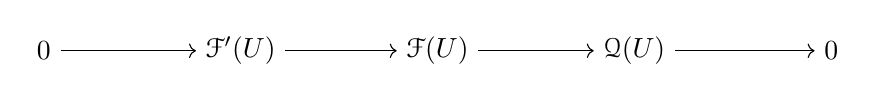
\begin{tikzpicture}[auto]
    \node (03) at (0,-1) {$0$};
    \node (im1) at (2.5,-1) {$\mathcal{F}'(U)$};
    \node (gu) at (5,-1) {$\mathcal{F}(U)$};
    \node (qu) at (7.5,-1) {$\mathcal{Q}(U)$};
    \node (04) at (10,-1) {$0$};

    \draw[->] (03) to (im1);
    \draw[->] (im1) to (gu);
    \draw[->] (gu) to (qu);
    \draw[->] (qu) to (04);
  \end{tikzpicture}
\end{center}
が作れる。帰納極限は完全列を完全列に移すので、またProp:\ref{Prop:1.3.7}より
\begin{center}
  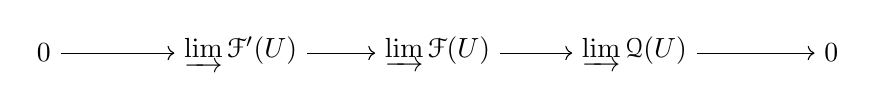
\begin{tikzpicture}[auto]
    \node (03) at (0,-1) {$0$};
    \node (im1) at (2.5,-1) {$\varinjlim \mathcal{F}'(U)$};
    \node (gu) at (5,-1) {$\varinjlim \mathcal{F}(U)$};
    \node (qu) at (7.5,-1) {$\varinjlim \mathcal{Q}(U)$};
    \node (04) at (10,-1) {$0$};

    \draw[->] (03) to (im1);
    \draw[->] (im1) to (gu);
    \draw[->] (gu) to (qu);
    \draw[->] (qu) to (04);
  \end{tikzpicture}
\end{center}
を得る。よって
\begin{center}
  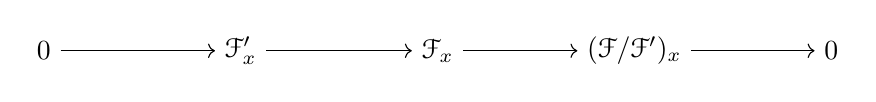
\begin{tikzpicture}[auto]
    \node (03) at (0,-1) {$0$};
    \node (im1) at (2.5,-1) {$\mathcal{F}'_{x}$};
    \node (gu) at (5,-1) {$\mathcal{F}_{x}$};
    \node (qu) at (7.5,-1) {$(\mathcal{F}/\mathcal{F}')_{x}$};
    \node (04) at (10,-1) {$0$};

    \draw[->] (03) to (im1);
    \draw[->] (im1) to (gu);
    \draw[->] (gu) to (qu);
    \draw[->] (qu) to (04);
  \end{tikzpicture}
\end{center}
したがって、
\begin{equation*}
  \mathcal{F}_{x}/\mathcal{F}'_{x} \simeq (\mathcal{F}/\mathcal{F}')_{x}
\end{equation*}
を得る。\\
次に
\begin{align*}
  (\ker \alpha)_{x}
    & = \{s_{x} \in \mathcal{F}_{x} \ |\ \alpha(U)(s) = 0,x\in U:\text{open},s\in \mathcal{F}(U) \}   \\
    & = \{s_{x} \in \mathcal{F}_{x} \ |\ \alpha_{x}(s_{x})=0,x\in U:\text{open},s\in \mathcal{F}(U)\} \\
    & = \ker \alpha_{x}
\end{align*}
を得る。同様に
\begin{align*}
  (\im \alpha)_{x}
    & = \{t_{x} \in \mathcal{G}_{x} \ |\ x\in \exists U:\text{open}, \exists s\in \mathcal{F}(U)\ \text{s.t}\ t = \alpha(U)(s)\} \\
    & = \{(\alpha(U)(s))_{x} \in \mathcal{G}_{x} \ |\ x \in U:\text{open},s\in \mathcal{F}(U)\}                                  \\
    & = \{\alpha_{x}(s_{x}) \in \mathcal{G}_{x}\ |\ s_{x} \in \mathcal{F}_{x}\}                                                  \\
    & = \im \alpha_{x}
\end{align*}
を得る.また,$(\mathcal{F}/\mathcal{F}')_{x} = \mathcal{F}_{x}/\mathcal{F}'_{x}$より
\begin{equation*}
  (\coker \alpha)_{x} = (\mathcal{G}/\im \alpha)_{x} = \mathcal{G}_{x}/\im \alpha_{x} = \coker \alpha_{x}
\end{equation*}
}

\Definition{
  層の列
  \begin{equation*}
    \mathcal{F} \stackrel{\alpha}{\longrightarrow} \mathcal{G} \stackrel{\beta}{\longrightarrow} \mathcal{H}
  \end{equation*}
  が完全とは、$\im \alpha = \ker \beta$が成り立つことをいう。
}
\Proposition{
  層の列に対して次が成り立つ。
  \begin{equation*}
    \mathcal{F} \longrightarrow \mathcal{G} \longrightarrow \mathcal{H}が完全
    \Longleftrightarrow
    任意のx \in Xに対して\mathcal{F}_{x} \longrightarrow \mathcal{G}_{x} \longrightarrow \mathcal{H}_{x}が完全
  \end{equation*}
}{
  Prop\ref{Prop:1.3.10}から明らか。
}

\Definition{
  $X,Y$を位相空間,$f:X\to Y$を連続写像とする。このとき、
  $X$上の層$\mathcal{F}$,$Y$上の層$\mathcal{G}$に対して、新たな$Y$上の層$f_{*}\mathcal{F}$が
  \begin{equation*}
    V \mapsto \mathcal{F}(f^{-1}(V))
  \end{equation*}
  によって定義できる。これを
  \index{そう@層!のじゅんぞう@の順像}\index{sheaf!direct image}
  \textbf{$\mathcal{F}$の順像(direct image of $\mathcal{F}$)}という。\\
  また、
  \begin{equation*}
    U \mapsto \varinjlim_{V\supset f(U)}\mathcal{G}(V)
  \end{equation*}
  で定義できる新たな$X$上の前層$f^{\cdot}\mathcal{G}$の層化$f^{-1}\mathcal{G}$を
  \index{そう@層!のぎゃくぞう@の逆像}\index{sheaf!inverse image}
  \textbf{$\mathcal{G}$の逆像(inverse image of $\mathcal{G}$)}
  という。
}

\Proposition{
  上の状況で
  \begin{equation*}
    (f^{-1}\mathcal{G})_{x} = \mathcal{G}_{f(x)} \qquad \forall x \in X
  \end{equation*}
}{
  \begin{equation*}
    (f^{-1}\mathcal{G})_{x} = \varinjlim_{x \in U}(f^{-1}\mathcal{G})(U) = \varinjlim_{x \in U}\varinjlim_{f(U) \subset V}\mathcal{G}(V) = \mathcal{G}_{f(x)}
  \end{equation*}
  最後の等号は明らか.
}

\Remark{
  $V$を$Y$の開集合とする。このとき自然な単射$i:V \to Y$に対して
  \begin{equation*}
    i^{-1}\mathcal{G} = \mathcal{G}|_{V}
  \end{equation*}
  が成り立つ。
}{}
\Proposition{
  $f:X \to Y$を位相空間の間の連続写像とし,$\mathcal{F}$を$X$上の層.$\mathcal{G}$を$Y$上の層とする.このとき
  \begin{equation*}
    \hom{\text{Sh}(X)}{f^{-1}\mathcal{G}}{\mathcal{F}}\simeq \hom{\text{Sh}(Y)}{\mathcal{G}}{f_{*}\mathcal{F}}
  \end{equation*}
  ただし,$\hom{\mathcal{C}}{X}{Y}$は圏$\mathcal{C}$で$X \to Y$なる射全体を表し,$\text{Sh}(X)$は$X$上の層全体を表す.
}{
  層化の普遍性より$\theta:f^{\cdot}\mathcal{G} \to f^{-1}\mathcal{G} = (f^{\cdot}\mathcal{G})^{\dagger}$
  を層化の射とすると,
  $$
    \begin{array}{rccc}
        & \hom{\text{PreSh}(X)}{f^{\cdot}\mathcal{G}}{\mathcal{F}} & \stackrel{\simeq}{\longrightarrow} & \displaystyle \hom{\text{Ph(X)}}{f^{-1}\mathcal{G}}{\mathcal{F}} \\
        & \rotatebox{90}{$\in$}                                    &                                    & \rotatebox{90}{$\in$}                                           \\
        & \alpha                                                   & \longmapsto                        & \tilde{\alpha}\circ \theta
    \end{array}
  $$
  が成り立つ.つまり
  \begin{equation*}
    \hom{\text{PreSh}(X)}{f^{\cdot}\mathcal{G}}{\mathcal{F}}\simeq \hom{\text{Sh(Y)}}{\mathcal{G}}{f_{*}\mathcal{F}}
  \end{equation*}
  を示せばいい.次に$X$上の開集合$U$に対して
  \begin{equation*}
    f^{\cdot}\mathcal{G}(U) = \varinjlim_{V\supset f(U)}\mathcal{G}(V)
  \end{equation*}
  なので,$\varphi \in \hom{\text{PreSh}(X)}{f^{\cdot}\mathcal{G}}{\mathcal{F}}$に対して
  \begin{equation*}
    \varphi(U) : \varinjlim_{V\supset f(U)}\mathcal{G}(V) \to \mathcal{F}(U)
  \end{equation*}
  を与えることは帰納極限の定義より$f(U)\subset V$なる開集合$V$に対して
  \begin{equation*}
    \psi'(V) : \mathcal{G}(V) \to \mathcal{F}(U)
  \end{equation*}
  を$f(U)\subset V' \subset V$ならば,
  \begin{equation*}
    \psi'(V) = \psi'(V')\circ \rho^{\mathcal{G}}_{V,V'}
  \end{equation*}
  となるように与えることである.すなわち$\psi'(V)$は
  \begin{equation*}
    \psi(V):\mathcal{G}(V) \to \mathcal{F}(f^{-1}(V))
  \end{equation*}
  と$\rho^{\mathcal{F}}_{f^{-1}(V),U}$を合成したものである.(帰納系の選び方によらない.)\\
  したがって,$\varphi\in \hom{\text{PreSh}(X)}{f^{\cdot}\mathcal{G}}{\mathcal{F}}$を与えることは,$\psi \in \hom{\text{Ph}(Y)}{\mathcal{G}}{f_{*}\mathcal{F}}$を与えることと等しい.
}

\Proposition{
  $\mathfrak{B}$を位相空間$X$の開基,$\mathcal{F},\mathcal{G}$を$X$上の層とする.このとき,すべての$U\in \mathfrak{B}$に対して,
  準同型$\alpha(U):\mathcal{F}(U) \to \mathcal{G}(U)$が定まっていて,制限写像と可換である.つまり
  \begin{equation*}
    \alpha(V)\circ \rho_{U,V}^{\mathcal{F}} = \rho_{U,V}^{\mathcal{G}}\circ \alpha(U)
  \end{equation*}
  となるとき,層の射$\alpha:\mathcal{F} \to \mathcal{G}$に唯一拡張できる.
}{
  $X$の任意の開集合$U$に対して$U_{i}\in \mathfrak{B}$なる開集合$U_{i}\subset U$たちが被覆する
  \begin{equation*}
    U = \bigcup_{i}U_{i}
  \end{equation*}
  で,もし層の射$\alpha:\mathcal{F}\to \mathcal{G}$があるならば
  制限写像と可換でなければならない.つまり
  \begin{equation*}
    \alpha(U_{i})\circ \rho_{U,U_{i}} = \rho_{U,U_{i}}\circ \alpha(U)
  \end{equation*}
  を満たすことに注意しよう.\\
  $\alpha(U_{i})$は定まっているのでそれらを張り合わせることによって,$\alpha(U)$を構成する.\\
  層の定義から$s\in \mathcal{F}(U)$に対して
  \begin{equation*}
    \alpha(U_{i})(s|_{U_{i}})\in \mathcal{G}(U_{i})
  \end{equation*}
  が定まる.仮定より各$\alpha(U_{i})$は制限写像と可換なので,
  \begin{align*}
    \alpha(U_{i})(s|_{U_{i}})|_{U_{i}\cap U_{j}} 
    &= \rho_{U_{i},U_{i}\cap U_{j}} \circ \alpha(U_{i})\circ \rho_{U,U_{i}}(s)\\
    &= \alpha(U_{i}\cap U_{j})\circ \rho_{U_{i},U_{i}\cap U_{j}}\circ \rho_{U,U_{i}}(s)\\
    &= \alpha(U_{i}\cap U_{j}) \circ \rho_{U,U_{i}\cap U_{j}}(s)\\
    &= \alpha(U_{i}\cap U_{j})(s|_{U_{i}\cap U_{j}})
  \end{align*}
  また,同様に
  \begin{align*}
    \alpha(U_{j})(s|_{U_{j}})|_{U_{i}\cap U_{j}}
    &= \rho_{U_{j},U_{i}\cap U_{j}}\circ \alpha(U_{j}) \circ \rho_{U,U_{j}}\\
    &= \alpha(U_{i}\cap U_{j}) \circ \rho_{U_{j},U_{i}\cap U_{j}}\circ \rho_{U,U_{j}}(s)\\
    &= \alpha(U_{i}\cap U_{j})\circ \rho_{U,U_{i}\cap U_{j}}(s)\\
    &= \alpha(U_{i}\cap U_{j})(s|_{U_{i}\cap U_{j}})
  \end{align*}
  したがって,
  \begin{equation*}
    \alpha(U_{i})(s|_{U_{i}})|_{U_{i}\cap U_{j}} = \alpha(U_{j})(s|_{U_{j}})|_{U_{i}\cap U_{j}}
  \end{equation*}
  だからGlueing local sections条件より
  \begin{equation*}
    t|_{U_{i}} = \alpha(U_{i})(s|_{U_{i}})
  \end{equation*}
  となる$t\in \mathcal{G}(U)$がある.また,Uniqueness条件よりこれは一意である.
  \begin{equation*}
    \alpha(U)(s) = t
  \end{equation*}
  とすれば,
  \begin{equation*}
    \alpha(U)(s)|_{U_{i}} = \alpha(U_{i})(s|_{U_{i}})
  \end{equation*}
  で,これはつまり制限写像と可換であり,$t$の一意性から$\alpha:\mathcal{F}\to \mathcal{G}$は唯一である.
}

\Example{
  $\mathcal{F}$を$X$上の層とする.このとき
  \begin{equation*}
    \text{Supp}\, \mathcal{F} = \{x\in X\mid \mathcal{F}_{x} \neq 0\}
  \end{equation*}
  と定義して\index{そう@層!のだい@の台}\index{sheaf!support}
  \textbf{$\mathcal{F}$の台(Supports of $\mathcal{F}$)}という.一般にはこれは閉集合ではない.
}{}

\subsection{$\mathfrak{B}$-sheaf}
$\mathfrak{B}$-sheafはアフィンスキームの構成にも必要な概念で,ラフに言えばすべての開集合$U$に対して$\mathcal{F}(U)$が定まっているものではなく,
開基$\mathfrak{B}$の元$U$に対してだけ定まっている層を$\mathfrak{B}$-sheafという.

\Definition{
  位相空間$X$の\textbf{開基$\mathfrak{B}$が有限交叉で閉じている}とは,任意の$U,V\in \mathfrak{B}$に対して$U\cap V \in \mathfrak{B}$が成り立つことをいう. 
}

\Example{
  環$A$の素イデアルの集合$\spec{A}$の基本開集合による開基$\{D(f)\}_{f\in A}$は有限交叉で閉じている.
}{}

\Definition{
  $X$を位相空間.$\mathfrak{B}$をその開基とする.このとき$\mathcal{F}$が
  \index{びーぜんそう@$\mathfrak{B}$-前層}\index{B-presheaf@$\mathfrak{B}$-presheaf}
  \textbf{$\mathfrak{B}$-前層($\mathfrak{B}$-presheaf)}であるとは,
  \begin{itemize}
    \item[---] $U\in \mathcal{B}$に対して$\mathcal{F}(U)$はアーベル群.
    \item[---] $V\subset U \in \mathcal{B}$に対して群準同型$\rho_{U,V}:\mathcal{F}(U) \to \mathcal{F}(V)$が定まる.
  \end{itemize}
  で,
  \begin{itemize}
    \item[(1)] $\rho_{U,U} = \text{id}_{\mathcal{F}(U)}$
    \item[(2)] 任意の開集合$W\subset V \subset U$に対して$\rho_{U,W} = \rho_{V,W}\circ \rho_{U,V}$となる.
  \end{itemize}
  を満たすときをいう.
}

\Definition{
  $\mathfrak{B}$が有限交叉で閉じているとする.このとき$\mathfrak{B}$-前層が層の条件を満たすとき
  \index{びーそう@$\mathfrak{B}$-層}\index{B-sheaf@$\mathfrak{B}$-sheaf}
  \textbf{$\mathfrak{B}$-層($\mathfrak{B}$-sheaf)}という.
}

\Proposition{
  $\mathcal{F}$を$\mathfrak{B}$-層とする.このとき,任意の$\mathfrak{B}$の元でない
  開集合$V$に対して
  \begin{equation*}
    \mathcal{F}(V) = \left\{(s_{U})_{U}\in \prod_{\substack{U \in \mathfrak{B} \\ U \subset V}}
    \mathcal{F}(U) \ \biggl|\ \forall U,U'\in \mathfrak{B},\ s_U|_{U\cap U'} = s_{U'}|_{U \cap U'}\right\}
  \end{equation*}
  とおく.演算を
  \begin{equation*}
    (s_U)_U + (t_U)_U = (s_U + t_U)_U
  \end{equation*}
  で定めるとアーベル群になる.\\
  また,$V'\subset V$に対して
  制限写像$\rho_{V,V'}:\mathcal{F}(V) \to \mathcal{F}(V')$を
  $(s_{U})_{U}\in \mathcal{F}(V)$を$V'\subsetneq U\subset V$なる$s_{U}$は無視
  するということで定義する.
  
  % \begin{align*}
  %   \mathcal{F}(V)
  %     & = \varprojlim_{\substack{U\in \mathcal{B}                  \\ U\subset V}}\mathcal{F}(U)\\
  %     & = \left\{(s_{U})_{U} \in \prod_{\substack{U\in \mathcal{B} \\ U \subset V}} \mathcal{F}(U) \ \biggl|\
  %   \forall U' \subset U \in \mathcal{B}, s_{U}|_{U'}=s_{U'} \right\}
  % \end{align*}
  % 制限写像は射影極限から誘導される射である.
  % \begin{center}
  %   \begin{tikzpicture}[auto]
  %     \node (X1) at (0,0) {$\mathcal{F}(U)$};
  %     \node (X2) at (0,-2.5) {$\displaystyle \varprojlim_{U\subset V}\mathcal{F}(U)$};
  %     \node (Y1) at (2.5,0) {$\mathcal{F}(U')$};
  %     \node (Y2) at (2.5,-2.5) {$\displaystyle \varprojlim_{U'\subset V'}\mathcal{F}(U')$};
  %     \node (ci) at (1.25,-1.25) {$\circlearrowleft$};
  
  %     \draw[->] (X1) to node[yshift = -6pt,label=above:$\rho_{U,U'}$] () {} (Y1);
  %     \draw[->] (X2) to node[xshift = 6pt, label=left:$\varphi_{U}$] () {} (X1);
  %     \draw[->] (X2) to node[yshift = -2pt,label=below:$\rho_{V,V'}$] () {} (Y2);
  %     \draw[->] (Y2) to node[xshift = 2pt,label=right:$\psi_{U'}$] () {} (Y1);
  %   \end{tikzpicture}
  % \end{center}
  % するとこれは前層になる.
}{
  \Claim{ (4)(Uniqueness)が成立する}\\
  $\mathfrak{B}$の元でない開集合$V$をとり開被覆$\{V_{i}\}_{i}$をとる.
  \begin{equation*}
    V = \bigcup_{\substack{V_{i} \subset V\\ V_{i} \in \mathfrak{B}}}V_{i} 
  \end{equation*}
  $s\in \mathcal{F}(V)$が任意の$i$に対して$s|_{V_{i}} = 0$とする.
  このとき$s= 0$が成り立つ.実際,定義から$s=0$とは
  $U\subset V$なる任意の$U\in \mathfrak{B}$に対して$s_{U}\in \mathcal{F}(U)$が$0$であること
  である.
  まず,$V$の開被覆から$U$の開被覆$\{U\cap V_{i}\}_{i} \subset \mathfrak{B}$を得る.
  また任意の$i$に対して$U\cap V_{i} \subset V_{i}$より$s|_{V_{i}}|_{U\cap V_{i}} = s|_{U\cap V_{i}} = 0$となる.従って任意の$i$に対して$s_{U}|_{U\cap V_{i}} = 0$となる.
  今$\mathcal{F}$は$\mathfrak{B}$-sheafなので$s_{U} = 0$よって$s=0$が分かる.\\
  \Claim{ (5)(Glueing local sections)が成立する}\\
  $s_{V_{i}} \in \mathcal{F}(V_{i})$が任意の$i,j$に対して$s_{V_{i}}|_{V_{i}\cap V_{j}} = s_{V_{j}}|_{V_{i} \cap V_{j}}$を満たすとする.
  $(s_{U})_{U}\in \prod \mathcal{F}(U)$を$U = V_{i}$のとき$s_{U} = s_{V_{i}}$で
  定義すれば,$(s_{U})_{U} \in \mathcal{F}(V)$で,$(s_{U})_{U}|_{V_{i}} = s_{V_{i}}$
}
% 位相空間$X$の任意の開集合$U$をとり,$\{U_{i}\}_{i}$をその開被覆とする.($U_{i} \in \mathcal{B}$)
% \begin{equation*}
%   \mathcal{F}(U):=\left\{(s_{i})_{i} \in \prod_{i}\mathcal{F}_0(U_{i})\ \Biggl|\ 任意のi,jに対してs_{i}|_{U_{i} \cap U_{j}} = s_{j}|_{U_{i} \cap U_{j}}\right\}
% \end{equation*}
% と定義する.するとこれは開被覆によらない.実際$\mathcal{F}(U)_{U_i}$を開被覆$\{U_{i}\}_{i}$による$\mathcal{F}(U)$とし,$\{V_{j}\}_{j}$を別の開被覆とすると,
% $\{U_{i}\cap V_{j}\}_{i,j}$はこれら2つの細分である.$\mathcal{F}(U)_{U_i} \to \mathcal{F}(U)_{U_{i}\cap V_{j}}$なる群準同型を
% $(s_{i})_{i}\mapsto (s_{i}|_{U_{i}\cap V_{j}})_{i,j}$で定義できる.実際
% \begin{align*}
%   s_{i} |_{U_{i} \cap V_{j}}\Bigl|_{(U_{i} \cap V_{j}) \cap (U_{i'} \cap V_{j'})}
%     & = s_{i} \Bigl|_{(U_{i} \cap V_{j}) \cap (U_{i'} \cap V_{j'})}                                                                              \\
%     & = s_{i} |_{U_{i}\cap U_{i'}}\Bigl|_{(U_{i} \cap V_{j}) \cap (U_{i'} \cap V_{j'})}                                                          \\
%     & = s_{i'} |_{U_{i}\cap U_{i'}}\Bigl|_{(U_{i} \cap V_{j}) \cap (U_{i'} \cap V_{j'})} \quad (\because (s_{i})_{i} \in \mathcal{F}(U)_{U_{i}}) \\
%     & = s_{i'} \Bigl|_{(U_{i} \cap V_{j}) \cap (U_{i'} \cap V_{j'})}                                                                             \\
%     & = s_{i'} |_{U_{i'} \cap V_{j'}}\Bigl|_{(U_{i} \cap V_{j}) \cap (U_{i'} \cap V_{j'})}
% \end{align*}
% より$(s_{i}|_{U_{i}\cap V_{j}})_{i,j}\in \mathcal{F}(U)_{U_{i} \cap V_{j}}$\\
% また,$(s_{ij})_{ij}\in \mathcal{F}(U)_{U_{i}\cap V_{j}}$を取ると,
% $(s_{ij})_{ij} = (s_{i}|_{U_{i} \cap V_{j}})$と出来るので全射(?????)\\
% Kernelを計算すると
% \begin{align*}
%     & s_{i}|_{U_{i}\cap V_{j}} = 0 \quad (\forall i,j)                \\
%     & s_{i}|_{U_{i}}=s_{i} = 0 \quad (\forall i) \quad (\because (4))
% \end{align*}
% よってKernelが自明なので単射.
% % $\mathcal{U}=\{U_{i}\}_{i}$を$X$の部分開集合族とする.$U=\cup_{i}U_{i},U_{ij}=U_{i}\cap U_{j}$

\Section{Ringed Topological Space}
\sectionmark{Ringed Topological Space}

\Definition{
  \index{きょくしょかんつきくうかん@局所環付き空間}\index{locally ringed space}
  \textbf{局所環付き空間}とは位相空間$X$と$X$上の環の層$\mathcal{O}_{X}$の組$(X,\mathcal{O}_{X})$
  で、任意の$x\in X$に対して$\mathcal{O}_{X,x}$が局所環となるものをいう。また、この$\mathcal{O}_{X}$
  を$(X,\mathcal{O}_{X})$の
  \index{こうぞうそう@構造層}\index{structure sheaf}
  \textbf{構造層(structure sheaf)}という。また$(X,\mathcal{O}_{X})$を単に
  $\mathcal{O}_{X}$と書くことがある。\\
  また、$\mathcal{O}_{X,x}$の唯一の極大イデアル$\mathfrak{m}_{x}$に対して
  その剰余体$\mathcal{O}_{X,x}/\mathfrak{m}_{x}$を
  \index{てんでのじょうよたい@点での剰余体}\index{residue field at point}
  \textbf{$X$の点$x$での剰余体(residue field of $X$ at $x$)}といって$k(x)$と書く。
}

\Definition{
\index{きょくしょかんつきくうかん@局所環付き空間!のしゃ@の射}\index{locally ringed space!morphism}
局所環付き空間の射とは
\begin{equation*}
  (f,f^{\#}): (X,\mathcal{O}_{X}) \to (Y,\mathcal{O}_{Y})
\end{equation*}
とは連続写像$f:X \to Y$と環の層の射$f^{\#}:\mathcal{O}_{Y} \to f_{*}\mathcal{O}_{X}$の組$(f,f^{\#})$で、
任意の$x\in X$に対して$f^{\#}_{x} : \mathcal{O}_{Y,f(x)} \to \mathcal{O}_{X,x}$は局所射となるものをいう。(つまり$f^{\#}_{x}(\mathfrak{m}_{Y,f(x)})\subset \mathfrak{m}_{X,x}$を満たす.)
}
Prop:\ref{Prop:1.3.13}より
\begin{equation*}
  f^{\#} : \mathcal{O}_{Y} \to f_{*}\mathcal{O}_{X}
\end{equation*}
を考えることは
\begin{equation*}
  f^{\#} : f^{*}\mathcal{O}_Y \to \mathcal{O}_{X}
\end{equation*}
を考えることに等しい.Def:\ref{Def:1.4.2}の$f^{\#}_{x}$は下の式で考えている.

\Definition{
\index{きょくしょかんつきくうかん@局所環付き空間!かいはめこみ@開はめ込み}\index{locally ringed space!open immersion}
射$(f,f^{\#}):(X,\mathcal{O}_{X}) \to (Y,\mathcal{O}_{Y})$が\textbf{開はめ込み(open immersion)}(resp. 
\index{きょくしょかんつきくうかん@局所環付き空間!へいはめこみ@閉はめ込み}\index{locally ringed space!closed immersion}
\textbf{閉はめ込み(closed immersion)})
とは連続写像$f$が開はめ込み(resp. 閉はめ込み)
\footnote{$f:X\to Y$が(位相的)開(閉)はめ込みとは$X$と$f(X)$が同相で$f(X)$が開(閉)集合のときをいう。}
でかつ任意の$x\in X$に対して$f^{\#}_{x}$が同型(resp. 全射)のときをいう。
}

\Definition{
  \index{いであるそう@イデアル層}\index{sheaf of ideals}
  $(X,\mathcal{O}_{X})$を局所環付き空間とする。$\mathcal{J}$が$\mathcal{O}_{X}$の
  \textbf{イデアル層(sheaf of ideals of $\mathcal{O}_{X}$)}とは任意の開集合$U$に対して
  $\mathcal{J}(U)$が$\mathcal{O}_{X}(U)$のイデアルになっているときをいう。
}

\Lemma{
$(X,\mathcal{O}_{X})$を局所環付き空間とする。$\mathcal{J}$を$\mathcal{O}_{X}$のイデアル層とする。
そして、
\begin{equation*}
  V(\mathcal{J}) = \{x \in X\ |\ \mathcal{J}_{x} \neq \mathcal{O}_{X,x}\}
\end{equation*}
とおく。(ちなみに上の諸々から$\mathcal{J}_{x} \subset \mathcal{O}_{X,x}$が分かる。)\\
$j:V(\mathcal{J}) \hookrightarrow X$を包含写像とする。すると
\begin{itemize}
  \item[---] $V(\mathcal{J})$は$X$の閉集合
  \item[---] $(V(\mathcal{J}),j^{*}(\mathcal{O}_{X}/\mathcal{J}))$は局所環付き空間
  \item[---] $j^{\#}$は自然な全射
        \begin{equation*}
          \mathcal{O}_{X} \longrightarrow \mathcal{O}_{X}/\mathcal{J} = j_{*}(j^{*}(\mathcal{O}_{X}/\mathcal{J}))
        \end{equation*}
        で
        $(j,j^{\#}):(V(\mathcal{J}),j^{-1}(\mathcal{O}_{X}/\mathcal{J})) \to (X,\mathcal{O}_{X})$は閉はめ込みである。
\end{itemize}
}{
\Claim{1}$V(\mathcal{J})$は$X$の閉集合\\
$x\in X\mysetminus V(\mathcal{J}) = \{x\in X\ |\ \mathcal{J}_{x} = \mathcal{O}_{X,x}\}$
に対して$f_{x} = 1$なる$x$の開近傍$U$と$f\in \mathcal{J}(U)$をとる。
つまり$f|_{V} = 1|_{V} = 1$なる$x$の開近傍$V \subset U$がある。
すると任意の$y \in V$に対して$f_{y} = 1 \in \mathcal{J}_{y}$となって,この$y$に対して
$\mathcal{J}_{y} = \mathcal{O}_{X,y}$なので
$V\subset X \mysetminus V(\mathcal{J})$となって$X\mysetminus V(\mathcal{J})$が開であることがわかる。\\
\Claim{2}$(V(\mathcal{J}),j^{*}(\mathcal{O}_{X}/\mathcal{J}))$は局所環付き空間\\
任意の$x\in V(\mathcal{J})$に対して
\begin{equation*}
  (j^{*}(\mathcal{O}_{X}/\mathcal{J}))_{x} = (\mathcal{O}_{X}/\mathcal{J})_{x} = \mathcal{O}_{X,x}/\mathcal{J}_{x}
\end{equation*}
は局所環。残りは自明。
}

\Proposition{
  $f:X \to Y$を局所環付き空間の閉はめ込みとする。$Z$を局所環付き空間$V(\mathcal{J})$とする。
  ただし、$\mathcal{J} = \ker f^{\#}\subset \mathcal{O}_{Y}$.すると$X\simeq Z$を自然な閉はめ込み
  $Z \hookrightarrow Y$から得る。
}{
  まず次の完全列
  \begin{equation*}
    0 \longrightarrow \mathcal{J} \longrightarrow \mathcal{O}_{Y} \longrightarrow f_{*}\mathcal{O}_{X} \longrightarrow 0
  \end{equation*}
  からProp:\ref{Prop:1.3.11}より任意の$y \in Y$に対して
  \begin{equation*}
    \mathcal{O}_{Y,y}/\mathcal{J}_{y} = (f_{*}\mathcal{O}_{X})_{y}
  \end{equation*}
  を得る。よって
  \begin{equation*}
    (f_{*}\mathcal{O}_{X})_{y} = \left\{
    \begin{alignedat}{2}
        & \quad 0 \qquad                           & y & \in Y \mysetminus V(\mathcal{J}) \\
        & \mathcal{O}_{Y,y}/\mathcal{J}_{y} \qquad & y & \in V(\mathcal{J})
    \end{alignedat}
    \right.\qquad \cdots (*)
  \end{equation*}
  を得る。$f(X)$は$Y$の閉集合なので$x\in Y\mysetminus f(X)$の開近傍$U$で
  \begin{equation*}
    f(X)\cap U = \varnothing
  \end{equation*}
  となるものがとれる。よって
  \begin{equation*}
    f_{*}\mathcal{O}_{X}(U) = \mathcal{O}_{X}(f^{-1}(U)) = \mathcal{O}_{X}(\varnothing) = 0
  \end{equation*}
  したがって、
  \begin{equation*}
    (f_{*}\mathcal{O}_{X})_{x} = 0
  \end{equation*}
  また、$y\in f(Y)$の開近傍$U$に対して$f$での引き戻し$f^{-1}(U)$は$y=f(x)$なる$x\in X$の開近傍である。
  これを$V$とおく。逆に、$f$は閉はめ込みなので、$X$は$f(X)$と同相なので$X$に自然に$Y$の相対位相が入る。
  つまり、任意の$x\in X$の開近傍$U$に対して$y=f(x)\in Y$の開近傍$V$が存在して$f^{-1}(V)$とかける。
  よって、
  \begin{equation*}
    (f_{*}\mathcal{O}_{X})_{y} = \varinjlim_{U \ni y}f_{*}\mathcal{O}_{X}(U) = \varinjlim_{U \ni y}\mathcal{O}_{X}(f^{-1}(U)) = \varinjlim_{V \ni x}\mathcal{O}_{X}(V) = \mathcal{O}_{X,x}
  \end{equation*}
  つまり、
  \begin{equation*}
    (f_{*}\mathcal{O}_{X})_{y} = \left\{
    \begin{alignedat}{2}
        & \quad 0 \qquad           & y & \in Y \mysetminus f(X) \\
        & \mathcal{O}_{X,x} \qquad & y & = f(x)
    \end{alignedat}
    \right.
  \end{equation*}
  $(*)$と比較すれば
  \begin{equation*}
    V(\mathcal{J}) = f(X)
  \end{equation*}
  が分かる。
  なので、$j:Z \hookrightarrow Y$を包含写像とすると、$f$から誘導される同相写像$g:X \to Z$に対して
  \begin{equation*}
    f = j \circ g
  \end{equation*}
  で、
  \begin{equation*}
    j_{*}\mathcal{O}_{Z} = \mathcal{O}_{Y}/\mathcal{J} \simeq f_{*}\mathcal{O}_{X}
  \end{equation*}
  がわかる。容易に
  \begin{equation*}
    f_{*}\mathcal{O}_{X} = j_{*}g_{*}\mathcal{O}_{X}
  \end{equation*}
  が分かるので
  \begin{equation*}
    \mathcal{O}_{Z} = (j^{-1}\circ j)_{*}\mathcal{O}_{Z} = (j^{-1})_{*}j_{*}\mathcal{O}_{Z}\simeq (j^{-1})_{*}j_{*}g_{*}\mathcal{O}_{X} = (j^{-1}\circ j)_{*} g_{*}\mathcal{O}_{X} = g_{*}\mathcal{O}_{X}
  \end{equation*}
  である。よって、$g$は局所環付き空間の同型射である。$f=j\circ g$が局所環付き空間の射であることを確認するのは読者に委ねる。
}

\Section{Schemes}
後できちんとした定義を述べるが,スキーム(scheme)とは局所環付き空間で局所的にはアフィンスキーム(affine scheme)とみれる
空間のことである.すなわち,先にアフィンスキームを定義せねばなるまい.\\
まず,$A$を環とし$X=\spec{A}$とし,Zariski位相が与えられてるとする.
このとき,$X$上の層$\mathcal{O}_{X}$を構成しよう.\\
まず,$D(f)\subset X$に対して$\mathcal{O}_{X}(D(f)) = A_{f}(=A[1/f])$とする.
次に射$\rho_{D(f),D(g)}:\mathcal{O}_{X}(D(f)) \to \mathcal{O}_{X}(D(g))$を定義しよう.\\
まず,$D(g) \subset D(f)$とする.つまり
\begin{equation*}
  g\in \sqrt{fA}
\end{equation*}
である.これは
\begin{equation}
  \exists m \in \mathbf{N}-\{0\},\exists b\in A\text{ s.t. } g^{m} = fb
\end{equation}
を意味する.よって$f$は$A_{g}$で単元である.実際上の式に両辺$1/g^{m}$をかけることによって
\begin{equation*} 
  f^{-1} = b/g^{m}
\end{equation*}
を得る.これによって制限写像$A_{f} \to A_{g}$を
\begin{equation*}
  a/f^{n} \mapsto ab^{n}/g^{mn}
\end{equation*}
で定義できる.もし$D(f) = D(g)$なら$A_{f} \to A_{g}$は同型射になる.(計算すれば容易にわかる.)
従って,$\mathcal{O}_{X}(D(f))$は$f$の選び方に依らない.$\{D(f)\}_{f}$は有限交叉で閉じた開基で
あったから,これは$\mathfrak{B}\text{-presheaf}$である.
\Proposition{
  $A$を環、$X=\text{Spec}\, A$とする。このとき以下が成り立つ。
  \begin{itemize}
    \item[(1)] $\mathcal{O}_{X}$を環の$\mathfrak{B}$-層とする。$\mathcal{O}_{X}$が誘導する$X$上の層$\mathcal{O}_{X}$は$\mathcal{O}_{X}(X)=A$となる。
    \item[(2)] 任意の$\mathfrak{p}\in X$に対して、茎$\mathcal{O}_{X,\mathfrak{p}}$は$A_{\mathfrak{p}}$への標準的な同型がある。特に、$(X,\mathcal{O}_{X})$は局所環付き空間になる。
  \end{itemize}
}{
  まず,$X = D(1)$なので$\mathcal{O}_{X}(X) = \mathcal{O}_{X}(D(1)) = A$.
  次に,開集合$U=X$についてUniquness条件を確認する.ほかの基本開集合も同様に示される.
  \begin{equation*}
    X = \bigcup_{i}D(f_{i}) = D(\sum_{i}f_{i}A)
  \end{equation*}
  開被覆$\{D(f_{i})\}_{i}$をとる.いま$s\in \mathcal{O}_{X}(X) = A$に対して
  $s|_{D(f_{i})} = 0$とする.このとき,ある$m_{i}\geq 1$があって,
  \begin{equation*}
    f_{i}^{m_{i}}s = 0
  \end{equation*}
  いま,
  \begin{equation*}
    X = \bigcup_{i}D(f_{i}) = \bigcup_{i}D(f^{m_{i}}_{i}) = D(\sum_{i}f^{m_{i}}_{i}A)
  \end{equation*}
  これは,$1 \in \sum f^{m_{i}}_{i}A$を意味する.よって
  \begin{equation*}
    s \in \sum_{i}sf^{m_{i}}_{i}A = 0
  \end{equation*}
  よって$s = 0$を得る.\\
  次に,Glueing local sections条件を確認する.
  $s_{i} \in \mathcal{O}_{X}(D(f_{i})) = A_{f_{i}}$をとる.
  そして,任意の$i,j$に対して,$s_{i}|_{D(f_{i})\cap D(f_{j})} = s_{j}|_{D(f_{i}) \cap D(f_{j})}$
  が成り立つとする.$s_{i} \in A_{f_{i}}$よりある$m_{i}\geq 1$があって
  \begin{equation*}
    s_{i} = \frac{b_{i}}{f^{m_{i}}_{i}}
  \end{equation*}
  実は$m_{i}$は$i$に関わらず選ぶことが出来る.$X$は準コンパクトなので有限個の$i\in I$で被覆できる.なので$\max \{m_{i}\}_{i \in I}$を$m$とすると,
  $m\geq m_{i}$なので,
  \begin{equation*}
    s_{i} = \frac{b_{i}}{f^{m_{i}}_{i}} = \frac{b_{i}f^{m - m_{i}}_{i}}{f^{m}_{i}} = \frac{c_{i}}{f^{m}_{i}}
  \end{equation*}
  となる.$D(f_{i})\cap D(f_{j}) = D(f_{i}f_{j})$であることを考慮すれば,
  \begin{align*}
    \left. \frac{b_{i}}{f^{m}_{i}} \right|_{D(f_{i}) \cap D(f_{j})} 
    &= \frac{b_{i}c_{i}^{m}}{(f^{n_{i}}_{i}f^{n_{i}}_{j})^{m}}\\
    \left. \frac{b_{j}}{f^{m}_{j}} \right|_{D(f_{i}) \cap D(f_{j})}
    &= \frac{b_{j}c_{j}^{m}}{(f^{n_{j}}_{i}f^{n_{j}}_{j})^{m}}
  \end{align*}
  よって,仮定から,
  \begin{equation*}
    \frac{b_{i}c_{i}^{m}}{(f^{n_{i}}_{i}f^{n_{i}}_{j})^{m}} = \frac{b_{j}c_{j}^{m}}{(f^{n_{j}}_{i}f^{n_{j}}_{j})^{m}}
  \end{equation*}
  なので,
  \begin{equation*}
    (f_{i}f_{j})^{r_{i,j}}(b_{i}c_{i}^{m}(f^{n_{j}}_{i}f^{n_{j}}_{j})^{m} - b_{j}c^{m}_{j}(f^{n_{i}}_{i}f^{n_{i}}_{j})^{m}) = 0
  \end{equation*}
  となる$r_{i,j}$がある.しかし,
  上と同様に$r = \max \{r_{i,j}\}_{(i,j)\in I\times I}$とおくと,
  \begin{equation*}
    (f_{i}f_{j})^{r}(b_{i}c_{i}^{m}(f_{i}^{n_{j}}f_{j}^{n_{j}})^{m} - b_{j}c_{j}^{m}(f_{i}^{n_{i}}f_{j}^{n_{i}})^{m}) = 0
  \end{equation*}
  で,
  上で見たように,$1 = \sum a_{j}f_{j}^{m+r_{i,j}}$なる$a_{j}\in A$
  がとれる.$s = \sum a_{j}b_{j}f^{r_{i,j}}_{j} \in A$とおくと,
  \begin{equation*}
    f^{m + r_{i,j}}_{i}s = \sum_{j}b_{j}f^{r_{i,j}}_{j}f^{m + r_{i,j}}_{i} = \sum_{j}a_{j}b_{i}f_{i}^{r_{i,j}}f_{j}^{m+r_{i,j}} = b_{i}f_{i}^{r_{i,j}}
  \end{equation*}
}

\Definition{
上で定義した局所環付き空間$(\text{Spec}\, A,\mathcal{O}_{\text{Spec}\, A})$を
\index{あふぃんすきーむ@アフィンスキーム}\index{affine scheme}
\textbf{アフィンスキーム(affine scheme)}という.
}

\Example{
  環$R$に対して$\mathbf{A}_{R}^{n}:=\spec{R[X_{1},\cdots,X_{n}]}$とおく.
  これを\textbf{$R$上の相対次元$n$のアフィン空間(affine space of relative dimension $n$ over $R$)}という.
  もちろん$(\mathbf{A}_{R}^{n},\mathcal{O}_{\mathbf{A}_{R}^{n}})$はアフィンスキーム
}{}

\Lemma{
  $A$を整域とし$K$をその商体とする.素イデアル$0$に対応する$X = \text{Spec}\, A$の点を$\xi$とする.このとき
  \begin{equation*}
    \mathcal{O}_{X,\xi} = K
  \end{equation*}
  が成り立つ.さらに,任意の空でない開集合$U \subset X$と$\xi \in U$に対して標準的な準同型
  \begin{equation*}
    \mathcal{O}_{X}(U) \to \mathcal{O}_{X,\xi}
  \end{equation*}
  は単射となる.開集合の組$V \subset U$に対して制限
  \begin{equation*}
    \mathcal{O}_{X}(U) \to \mathcal{O}_{X}(V)
  \end{equation*}
  は単射となる.
}{
  Prop:\ref{Prop:1.5.1}(2)より
  \begin{equation*}
    \mathcal{O}_{X,\xi} = A_{\xi} = K
  \end{equation*}
  を得る.\\
  $U=D(f)$とすると,$\mathcal{O}_{X}(U) = A_{f}\subset K$.一般に
  \begin{equation*}
    U = \bigcup_{i}D(f_{i})
  \end{equation*}
  と置く.$s\in \mathcal{O}_{X}(U)$を飛ばすと$0 \in K$になるとする.各開被覆$D(f_{i}) \subset U$への
  制限を考えると
  \begin{equation*}
    s|_{D(f_{i})} = 0
  \end{equation*}
  が任意の$i$で成り立つので,$s=0$である.よって$\mathcal{O}_{X}(U) \to \mathcal{O}_{X,\xi} \subset K$は単射.\\
  開集合の組$\xi \in V\subset U$に対して制限$\mathcal{O}_{X}(U) \to \mathcal{O}_{X}(V)$に対して帰納極限の定義より図式
  \begin{center}
    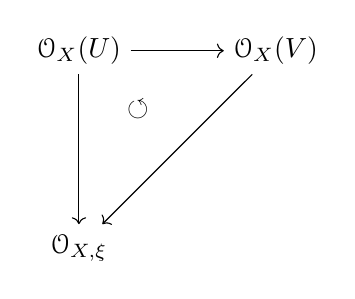
\begin{tikzpicture}[auto]
      \node (OU) at (0,0) {$\mathcal{O}_{X}(U)$};
      \node (Oxi) at (0,-2.5) {$\mathcal{O}_{X,\xi}$};
      \node (OV) at (2.5,0) {$\mathcal{O}_{X}(V)$};
      \node (ci) at (0.75,-0.75) {$\circlearrowleft$};

      \draw[->] (OU) to node () {} (OV);
      \draw[->] (OU) to node () {} (Oxi);
      \draw[->] (OV) to node () {} (Oxi);
    \end{tikzpicture}
  \end{center}
  が可換となるので,制限は単射である.
}

\Lemma{
$X = \text{Spec}\, A$をアフィンスキームとし,$g\in A$をとる.このとき開集合$D(g)$は
$X$から誘導される局所環付き空間で$\spec{A_{g}}$に同型なアフィンスキームになる.
}{
$Y = \spec{A_{g}}$と置く.局所化と素イデアルの対応より標準的な開はめ込み
\begin{equation*}
  i:Y \to X
\end{equation*}
がある($\im i = D(g)$)\\
$D(h)\subset D(g)$とする.$A\stackrel{\varphi}{\longrightarrow} A_{g}$とする.また$\varphi(h) = \bar{h}$と置く.このとき標準的な同型
\begin{equation*}
  \mathcal{O}_{X}(D(h)) = A_{h} \simeq (A_{g})_{\bar{h}} = \mathcal{O}_{Y}(D(\bar{h})) = i_{*}\mathcal{O}_{Y}(D(h))
\end{equation*}
今$A_{h}\simeq (A_{g})_{\bar{h}}$は感覚的には
\begin{equation*}
  (A_{g})_{\bar{h}} = (A[1/g])_{\bar{h}} = A[1/g,1/\bar{h}]
\end{equation*}
で,$D(h)\subset D(g)$より$h^{n} = gb$となる$n\in \mathbf{N}-\{0\}$と$b\in A$がある.よって
\begin{equation*}
  A[1/g,1/\bar{h}] = A[b/h^{n},1/\bar{h}] = A[1/h]=A_{h}
\end{equation*}
具体的にはまず,$\varphi$が単射ではないとき,
\begin{equation*}
  \ker{\varphi} \neq 0 \Leftrightarrow A_{g} = 0
\end{equation*}
に注意すると(よって$(A_{g})_{\bar{h}} = 0$),定義から$\ker{\varphi} \ni a \neq 0$とすると
\begin{equation*}
  \exists m\in \mathbf{N}\text{ s.t. } g^{m}a = 0
\end{equation*}
を満たす.また$h^n = gb$より$h^{nm}a = g^{m}ab^{m} = 0$より$\ker{(A\to A_{h})}$は$0$でない.
従って,$A_{h}=0$だから自明に同型である.よって$\varphi$を単射とする.\\
\begin{equation*}
  (A_{g})_{\bar{h}} \to A_{h}
\end{equation*}
を,
\begin{equation*}
  \frac{a}{g^{m}}\frac{1}{\bar{h}^{k}} \mapsto \frac{ab^{m}}{h^{mn}}\frac{1}{h^{k}} = \frac{ab^{m}}{h^{mn + k}}
\end{equation*}
で定義する.これは簡単に準同型であることがわかる.次に
\begin{equation*}
  A_{h} \to (A_{g})_{\bar{h}}
\end{equation*}
を,
\begin{equation*}
  \frac{a}{h^{n}} \mapsto \frac{\bar{a}}{\bar{h}^{n}}
\end{equation*}
で定義する.これらは互いに逆射を与えるので,$(A_{g})_{\bar{h}}\simeq A_{h}$を得る.\\
$\{D(h)\}_{h}$は$D(g)$の開基となるので,$i$は$(Y,\mathcal{O}_{Y})$から$(D(g),\mathcal{O}_{X}|_{D(g)})\subset (X,\mathcal{O}_{X})$
への同型を誘導する.(Refer to Exercises 2.7)
}

\Definition{
\index{すきーむ@スキーム}\index{scheme}
\textbf{スキーム(scheme)}とは局所環付き空間$(X,\mathcal{O}_{X})$で開被覆$\{U_{i}\}_{i}$に対して$(U_{i},\mathcal{O}_{X}|_{U_{i}})$
がアフィンスキームになるものが存在するときをいう.また$\mathcal{O}_{X}(U)$の元は(やや不適切であるが)
\index{せいそくかんすう@正則関数}\index{regular function}
\textbf{$U$上の正則関数(regular functions on $U$)}という.しかし,層の関数としての側面をよく表している.(Refer to Exercises 3.4 and Proposition 4.4)
}

明らかにアフィンスキームはスキームである.また,局所環付き空間$X$が開被覆$\{U_{i}\}_{i}$に対して
$(U_{i},\mathcal{O}_{X}|_{U_{i}})$がスキームだったら$X$はスキームである.逆に次の命題が従う.

\Proposition{
$X$をスキームとする.このとき任意の開集合$U\subset X$に対して局所環付き空間$(U,\mathcal{O}_{X}|_{U})$はまたスキームになる.
}{
定義より$X = \bigcup_{i}U_{i}$で$U_{i}$は開集合で,アフィンスキームになるものがある.
$U\cap U_{i}$がスキームとなることを示せば十分である.
}

\Definition{
$X$をスキームとする.$U$を$X$の開集合とする.スキーム$(U,\mathcal{O}_{X}|_{U})$を$X$の
\index{かいぶぶんすきーむ@開部分スキーム}\index{open subscheme}
\textbf{開部分スキーム(open subscheme)}
更に$(U,\mathcal{O}_{X}|_{U})$がアフィンスキームになるとき$U$を
\index{あふぃんかいしゅうごう@アフィン開集合}\index{affine open subset}
\textbf{アフィン開集合(affine open subset)}という.
}

以下,$X$の開集合$U$はスキームの構造が与えられているとする.

\Definition{
  $X$をスキーム,$f\in \mathcal{O}_{X}(X)$とする.
  \begin{equation*}
    X_{f}:= \{x\in X\ |\ f_{x} \in \mathcal{O}^{\times}_{X,x}\}
  \end{equation*}
  ただし,$A^{\times}$は$A$の単元群である.(LiuのDefinition 3.11.では*の記号を用いている.)
}

次の条件を考えよう.

\begin{conditionbox}
  $X$は有限アフィン開被覆$\{U_{i}\}_{i}$があって$U_{i}\cap U_{j}$はまた有限アフィン開被覆を持つ.
\end{conditionbox}
便宜上この条件を条件Aと呼称する.



\Proposition{
$X$をスキームとし$f\in \mathcal{O}_{X}(X)$とする.このとき$X_{f}$は$X$の開集合で,
更に,$X$が条件Aを満たすなら,制限$\mathcal{O}_{X}(X)\to \mathcal{O}_{X}(X_{f})$は同型
\begin{equation*}
  \mathcal{O}_{X}(X)_{f} \simeq \mathcal{O}_{X}(X_{f})
\end{equation*}
を誘導する.
}{
$x\in X_{f}$とする.$x$の開近傍$U$と$g\in \mathcal{O}_{X}(U)$があって,$f_{x}g_{x} = 1$を満たすものがある.
$f_{x}g_{x} = (fg)_{x}$よりある$x$の開近傍$V\subset U$があって$fg|_{V}=1$を満たす.
したがって,$V\subset X_{f}$となる.よって$X_{f}$は開集合である.\\
更に,$V$が動くにつれて$f$の逆元$g\in \mathcal{O}_{X}(V)$を張り合わせると
$f|_{X_{f}}$の$\mathcal{O}_{X}(X_{f})$での逆元を得る.\\
詳しく言えば,$X_{f}$の上の$V$を集めた開被覆$\{V_{i}\}_{i}$を取り,$fg_{i}|_{V_{i}} = 1$なる$g_{i} \in \mathcal{O}_{X}(V_{i})$を考えれば
任意の$i,j$に対して
\begin{equation*}
fg_{i}|_{V_{i} \cap V_{j}} = 1 = fg_{j}|_{V_{i} \cap V_{j}}
\end{equation*}
より
\begin{align*}
(左辺) - (右辺) 
&= fg_{i}|_{V_{i} \cap V_{j}} - fg_{j}|_{V_{i} \cap V_{j}}\\
&= f|_{V_{i} \cap V_{j}}(g_{i}|_{V_{i} \cap V_{j}} - g_{j}|_{V_{i} \cap V_{j}})\\
&= 0
\end{align*}
また,$f|_{V_{i}}$は単元なので逆元$(f|_{V_{i}})^{-1}$がある.また,
\begin{equation*}
f|_{V_{i} \cap V_{j}} = (f|_{V_{i}})|_{V_{i} \cap V_{j}}
\end{equation*}
なので,
\begin{align*}
f|_{V_{i} \cap V_{j}} ((f|_{V_{i}})^{-1}|_{V_{i} \cap V_{j}}) 
&= (f|_{V_{i}})|_{V_{i} \cap V_{j}} ((f|_{V_{i}})^{-1}|_{V_{i} \cap V_{j}}) \\
&= ((f|_{V_{i}})(f|_{V_{i}})^{-1})|_{V_{i} \cap V_{j}} \\
&= 1
\end{align*}
よって$f|_{V_{i} \cap V_{j}}$はまた単元で$g_{i}|_{V_{i} \cap V_{j}} = g_{j}|_{V_{i} \cap V_{j}}$を得る.

$\mathcal{O}_{X}$は層なので,貼り合わせ条件より$g|_{V_{i}} = g_{i}$なる$g\in \mathcal{O}_{X}(X_{f})$がある.
この$g$が$f|_{X_{f}}$の逆元になっている.\\
よって制限$\mathcal{O}_{X}(X)\to \mathcal{O}_{X}(X_{f})$
から準同型
\begin{equation*}
\alpha : \mathcal{O}_{X}(X)_{f}\to \mathcal{O}_{X}(X_{f});\frac{x}{f^n} \mapsto \rho_{X,X_f}(x)f^{-n} = \rho_{X,X_f}(x)g^n
\end{equation*}
を誘導する.($\mathcal{O}_{X}(X)$は環なので$\mathcal{O}_{X}(X)_{f}$は$\{f^{n}\}_{n\in \mathbf{N}}$での局所化であることに注意しよう.)
ここで条件Aを仮定すれば,$X$は有限アフィン開被覆$\mathcal{U} = \{U_{i}\}_{i}$を持つ.
よって,
\begin{equation*}
X_{f} = \bigcup_{i}U_{i}\cap X_{f} = \bigcup_{i}V_{i} = \bigcup_{i}D(f|_{U_{i}})
\end{equation*}
ここで,$U_{i} = \spec{A_{i}}$とすると
\begin{align*}
  U_{i} \cap X_{f} 
  &= \{x\in X\cap \spec{A_{i}}\mid f_{x} \in \mathcal{O}_{X,x}^{\times}\}\\
  &= \{x\in \spec{A_{i}}\mid f_{x} \in \mathcal{O}_{X,x}^{\times}\}\\
  &= \{x\in \spec{A_{i}}\mid f_{x} \in (\mathcal{O}_{X}|_{\spec{A_{i}},x})^{\times}\}\\
  &= \{\mathfrak{p}\in \spec{A_{i}}\mid f_{\mathfrak{p}} \in A_{i,\mathfrak{p}}^{\times}\}
\end{align*}
ここで,素イデアルの局所化$A_{\mathfrak{p}}$が局所環でその極大イデアルが
$A_{\mathfrak{p}}\mysetminus A_{\mathfrak{p}}^{\times} = \mathfrak{p}A_{\mathfrak{p}}$となることに注意すると
\begin{align*}
  \{\mathfrak{p} \in \spec{A_{i}}\mid f_{\mathfrak{p}}\in A_{i,\mathfrak{p}}^{\times}\}
  &= \{\mathfrak{p} \in \spec{A_{i}} \mid f_{\mathfrak{p}} \notin \mathfrak{p}A_{i,\mathfrak{p}}\}\\
  &= \{\}
\end{align*}
%D(f|_{U_{i}})がなぞ
Lem:\ref{Lem:1.5.3}より$\mathcal{O}_{X}(U_{i})_{f} = \mathcal{O}_{X}(V_{i})$\\
今以下の完全系列を得る.
\begin{equation*}
C^{\bullet}(\mathcal{U},\mathcal{O}_{X}):0 \longrightarrow \mathcal{O}_{X}(X) \stackrel{d_{0}}{\longrightarrow} \bigoplus_{i}\mathcal{O}_{X}(U_{i}) \stackrel{d_{1}}{\longrightarrow} \bigoplus_{i,j}\mathcal{O}_{X}(U_{i} \cap U_{j})
\end{equation*}
ただし$d_{0}:s\mapsto (s|_{U_{i}})_{i},d_{1}:(s_{i})_{i}\mapsto (s_{i}|_{U_{i}\cap U_{j}} - s_{j}|_{U_{i} \cap U_{j}})_{i,j}$
とする.(有限個なら直積$\prod$と直和$\bigoplus$は同じ)\\
次にテンソルをとることは左完全関手なので$C^{\bullet}(\mathcal{U},\mathcal{O}_{X})\otimes_{\mathcal{O}_{X}(X)}\mathcal{O}_{X}(X)_{f}$
はまた,完全列である.よってこれは次の可換図式を与える.

\begin{center}
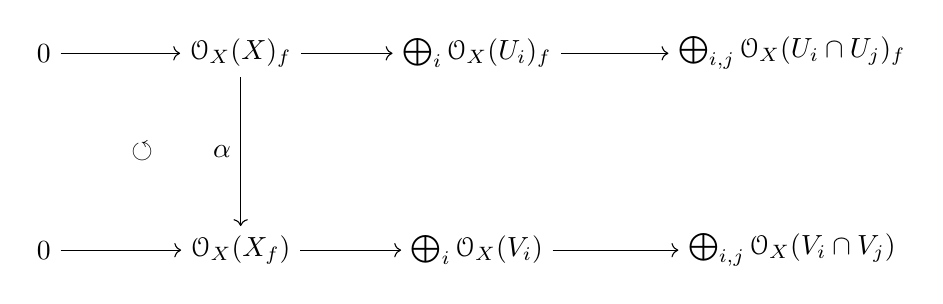
\begin{tikzpicture}[auto]
  \node (00) at (0,0) {$0$};
  \node (01) at (0,-2.5) {$0$};
  \node (OX_f) at (2.5,0) {$\mathcal{O}_{X}(X)_{f}$};
  \node (OXf_) at (2.5,-2.5) {$\mathcal{O}_{X}(X_{f})$};
  \node (oOU_f) at (5.5,0) {$\bigoplus_{i}\mathcal{O}_{X}(U_{i})_{f}$};
  \node (oOV) at (5.5,-2.5) {$\bigoplus_{i}\mathcal{O}_{X}(V_{i})$};
  \node (oOUU_f) at (9.5,0) {$\bigoplus_{i,j}\mathcal{O}_{X}(U_{i}\cap U_{j})_{f}$};
  \node (oOVV) at (9.5,-2.5) {$\bigoplus_{i,j}\mathcal{O}_{X}(V_{i}\cap V_{j})$};
  \node (ci) at (1.25,-1.25) {$\circlearrowleft$};

  \draw[->] (00) to (OX_f);
  \draw[->] (01) to (OXf_);
  \draw[->] (OX_f) to (oOU_f);
  \draw[->] (OXf_) to (oOV);
  \draw[->] (oOU_f) to (oOUU_f);
  \draw[->] (oOV) to (oOVV);
  \draw[->] (OX_f) to node[label=left:$\alpha$] () {} (OXf_);
  % \draw[->] (X2) to node[yshift = -2pt,label=below:$f_{\lambda}$] () {} (Y2);
  % \draw[->] (Y1) to node[xshift = -6pt,label=right:$\psi_{\lambda,\mu}$] () {} (Y2);
\end{tikzpicture}
\end{center}
}

\subsection{Morphism of schemes}
\sectionmark{Morphism of schemes}
\Definition{
  \index{すきーむ@スキーム!のしゃ@の射}\index{scheme!morphism}
  $f:X\to Y$が\textbf{スキームの射(morphism of schemes)}とは局所環付き空間としての射とする.
}

環の射$\varphi:A\to B$が誘導する射$\spec{B} \to \spec{A}$を$\varphi^{a}$と書くことにする.\\
つまり$\mathfrak{p}\in \spec{B}$に対して$\varphi^{a}(\mathfrak{p}) = \varphi^{-1}(\mathfrak{p})$

\Proposition{
  $\varphi: A \to B$を環の射とする.このとき
  \begin{equation*}
    (\varphi^{a},(\varphi^{a})^{\#}):\spec{B} \to \spec{A}
  \end{equation*}
  は$(\varphi^{a})^{\#}(\spec{A})=\varphi$を満たすスキームの射である.
}{
  $X=\spec{B},Y=\spec{A}$と置く.任意の$f\in A$に対して
  \begin{equation*}
    (\varphi^{a})^{-1}(D(f))=D(\varphi(f))
  \end{equation*}
  が成り立ち,実際
  \begin{align*}
    (\varphi^{a})^{-1}(D(f)) 
    &= \{ \mathfrak{p} \in X\ |\ \varphi^{a}(\mathfrak{p}) \in D(f)\}\\
    &= \{ \mathfrak{p} \in X\ |\ f \notin \varphi^{a}(\mathfrak{p})\}\\
    &= \{ \mathfrak{p} \in X \mid f \notin \varphi^{-1}(\mathfrak{p})\}\\
    &= \{ \mathfrak{p} \in X \mid \varphi(f) \notin \mathfrak{p}\}\\
    &= D(\varphi(f))
  \end{align*}  
  である.$\varphi$から誘導される環の射
  \begin{equation*}
    (\varphi^{a})^{\#}(D(f)):\mathcal{O}_{Y}(D(f)) = A_{f} \to B_{\varphi(f)} = \mathcal{O}_{X}(D(\varphi(f))) = (\varphi^{a})_{*}\mathcal{O}_{X}(D(f))
  \end{equation*}
  これは制限写像と可換(compatibleという意味で)になる.よって層の射
  \begin{equation*}
    (\varphi^{a})^{\#}:\mathcal{O}_{Y} \to \varphi^{a}_{*}\mathcal{O}_{X}
  \end{equation*}
  に拡張できる.
  %開基?(or 基本開集合族)で決まっていれば拡張できることを証明する.
  更に,任意の$\mathfrak{q} \in X$に対して$\varphi$から誘導される環の射
  \begin{equation*}
    (\varphi^{a})^{\#}_{\mathfrak{q}}:A_{\varphi^{a}(\mathfrak{q})} \to B_{\mathfrak{q}}
  \end{equation*}
  は局所射で,実際
  \begin{align*}
    (\varphi^{a})^{\#}_{\mathfrak{q}}(\varphi^{a}(\mathfrak{q})A_{\varphi^{a}(\mathfrak{q})})
    &= \{ \varphi(a)/\varphi(p) \mid a\in \varphi^{a}(\mathfrak{q}),p \notin \varphi^{a}(\mathfrak{q})\}\\
    &= \{\varphi(a)/\varphi(p)\mid \varphi(a)\in \mathfrak{q},\varphi(p)\notin \mathfrak{q}\}\\
    &\subset \{b/q\mid b\in \mathfrak{q},q\notin \mathfrak{q}\}\\
    &= \mathfrak{q}B_{\mathfrak{q}}
  \end{align*}
  よって$(\varphi^{a},(\varphi^{a})^{\#})$は
  局所環付き空間の射になる.$D(1) = Y$だから,構成により
  \begin{equation*}
    (\varphi^{a})^{\#}(Y):\mathcal{O}_{Y}(Y) = A \to B = \mathcal{O}_{X}(X) = (\varphi^{a})_{*}\mathcal{O}_{X}(Y)
  \end{equation*}
  で$(\varphi^{a})^{\#}(Y) = \varphi$を満たす.
}

\Example{
  $A$を環とする.$f\in A$に対して$\varphi:A\to A_{f}$を自然な射とする.よってProp:\ref{Prop:1.5.7}より
  $\varphi^{a}:\spec{A_{f}} \to \spec{A}$はアフィンスキームの射で,$\spec{A_{f}}\simeq D(f)$
  で,$D(f)\to \spec{A}$は開はめ込みである.
}{}

\Example{
  $X$をスキームとする.$x\in X$に対して標準的な射$\spec{\mathcal{O}_{X,x}} \to X$がある.
  実際$x\in U$なるアフィン開集合に対して標準的な射$\mathcal{O}_{X}(U) \to \mathcal{O}_{X,x}$
  から誘導される射$\spec{\mathcal{O}_{X,x}} \to \spec{\mathcal{O}_{X}(U)} = U$
  がとれる.また$U\hookrightarrow X$は自然に開はめ込みだと見れるので射$\spec{\mathcal{O}_{X,x}} \to X$
  を得る.これは$U$の選び方に依らない.
}{}

\Lemma{
  $A$を環とし,$I$をそのイデアルとする.このとき,スキームの射
  \begin{equation*}
    i:\spec{A/I} \to \spec{A}
  \end{equation*}
  が自然な射影$\varphi:A\to A/I$によって誘導される.$i$は$\im{i} = V(I)$へのスキームの閉はめ込みである.
  更に,任意の$\spec{A}$の基本開集合$D(f)$に対して
  \begin{equation*}
    (\ker{i^{\#}})(D(f)) = I\otimes_{A}A_{f}
  \end{equation*}
  が成り立つ.
}{
  $i$が閉はめ込みであることはよい.次に,任意の$\spec{A}$の基本開集合$D(f)$に対して先ほど
  みたように,標準的な全射
  \begin{equation*}
    \mathcal{O}_{\spec{A}}(D(f)) = A_{f} \to (A/I)_{\varphi(f)} = i_{*}\mathcal{O}_{\spec{A/I}}(D(f))
  \end{equation*}
  がある.これにより,$i^{\#}$の全射性と,
  \begin{align*}
    (\ker{i^{\#}})(D(f)) 
    &= \ker{(i^{\#}(D(f)))}\\
    &= \ker{(A_{f} \to (A/I)_{\varphi(f)})}\\
    &= I_{f} \\
    &= I\otimes_{A}A_{f}
  \end{align*}
  がわかる.
}

\Example{
  $X$をスキームとする.$x\in X$に対して$k(x)$は点$x$での$X$の剰余体であった.(Def:\ref{Def:1.4.1}を参照.)このとき標準的な全射$\varphi:\mathcal{O}_{X,x} \to k(x) = \mathcal{O}_{X,x}/\mathfrak{m}_{x}$
  は閉はめ込み$i:\spec{k(x)} \to \spec{\mathcal{O}_{X,x}}$を誘導する.Ex:\ref{Ex:1.5.9}より
  射$\spec{\mathcal{O}_{X,x}} \to X$がある.よって射$f:\spec{k(x)} \to X$を得る.この射は$\spec{k(x)}$の
  唯一の点を$x\in X$に送る射である.\\
  $x\in \spec{k(x)}$を取ると$(f\circ i)(x) = f(\varphi^{-1}(x)) = $
}{}

\Definition{
  $Z$を$X$の閉集合とする.このとき$Z$が
  \index{へいぶぶんすきーむ@閉部分スキーム}\index{closed subscheme}
  \textbf{閉部分スキーム(closed subscheme)}とは
  包含写像$j:Z\to X$が閉はめ込み
  \begin{equation*}
    (j,j^{\#}):(Z,\mathcal{O}_{Z}) \to (X,\mathcal{O}_{X})
  \end{equation*}
  となるときをいう.
}



\Proposition{
  $X=\spec{A}$をアフィンスキームとする.$j:Z\to X$をスキームの閉はめ込みとする.
  このとき,$Z$はアフィンスキームで,あるイデアル$J\subset A$が唯一存在して
  $j$は同型$Z\stackrel{\simeq}{\longrightarrow}\spec{A/J}$を誘導する.
}{}

\Definition{
  $S$をスキームとする.このとき$X$が
  \index{えすすきーむ/えすじょうのすきーむ@$S$-スキーム/$S$上のスキーム}
  \index{S-scheme/scheme over S@$S$-scheme/scheme over $S$}
  \textbf{$S$-スキーム($S$-scheme)}または\textbf{$S$上のスキーム(scheme over $S$)}とは
  スキームの射$\pi:X \to S$が与えられているときをいう.この$\pi$を
  \index{こうぞうしゃ@構造射}\index{structural morphism}
  \textbf{構造射(structural morphism,\ structure morphism)}
  ,$S$を
  \index{きていすきーむ@基底スキーム}\index{base scheme}
  \textbf{基底スキーム(base scheme)}という.$S=\spec{A}$のときまた$X$を
  \index{えーすきーむ/えーじょうのすきーむ@$A$-スキーム/$A$上のスキーム}\index{A-scheme/scheme over A@$A$-scheme/scheme over $A$}
  \textbf{$A$-スキーム($A$-scheme)}または\textbf{$A$上のスキーム(scheme over $A$)}
  という.このとき$A$を\index{きていかん@基底環}\index{base ring}\textbf{基底環(base ring)}
}

\Definition{
  $\pi:X\to S,\rho:Y \to S$を$S$上のスキームとする.このとき
  \index{えすすきーむ/えすじょうのすきーむ@$S$-スキーム/$S$上のスキーム!のしゃ@の射}
  \index{S-scheme/scheme over S@$S$-scheme/scheme over $S$!morphism}
  \textbf{$S$-スキームの射(morphism of $S$-scheme)}$f:X\to Y$とは$f$がスキームの射で
  $\rho \circ f = \pi$を満たすことをいう.
}

スキーム$X,Y$に対して
\begin{equation*}
  \hom{\textbf{Sch}}{X}{Y}:=\{f:X\to Y\ |\ f\text{ is morphism of schemes}\}
\end{equation*}
また,環$A,B$に対して
\begin{equation*}
  \hom{\textbf{Ring}}{A}{B}:=\{f:A\to B\ |\ f\text{ is morphism of rings}\}
\end{equation*}
とおく.このとき標準的な写像
\begin{equation*}
  \rho:\hom{\textbf{Sch}}{X}{Y} \to \hom{\textbf{Ring}}{\mathcal{O}_{Y}(Y)}{\mathcal{O}_{X}(X)}
\end{equation*}
がある.実際$(f,f^{\#})\in \hom{\textbf{Sch}}{X}{Y}$とすると
\begin{equation*}f^{\#}(Y):\mathcal{O}_{Y}(Y) \to f_{*}\mathcal{O}_{X}(Y) = \mathcal{O}_{X}(f^{-1}(Y))=\mathcal{O}_{X}(X)
\end{equation*}
がある.
%関手的であることを確認する.


\Definition{
  $\pi:X\to S$を$S$上のスキームとする.\textbf{$X$の切断(section of $X$)}\index{せつだん@切断}
  \index{section}とは$S$上のスキームの射$\sigma:S\to X$で$\pi \circ \sigma=\text{id}_S$となるときをいう.
  $X$の切断の集合を$X(S)$($S=\spec{A}$のときは$X(A)$)とかく.
}

\Example{
  $X$を体$k$上のスキームとする.このとき
  \begin{equation*}
    X(k) = \{x\in X\mid k(x) = k\}
  \end{equation*}
  実際$\sigma\in X(k)$をとる.$\mathcal{O}_{\spec{k},(0)} = k_{(0)} = k$より
  \begin{equation*}
    \sigma^{\#}_{(0)}:\mathcal{O}_{X,\sigma((0))}\to \mathcal{O}_{\spec{k},(0)} = k
  \end{equation*}
  で,
}{}

\Definition{
  $X$を体$k$上のスキームとする.上の例より$X(k)$の点を\index{ゆうりてん@有理点}\index{rational points}
  \textbf{$X$の$k$-有理点($k$-rational points of $X$)}という.
}

\Remark{
  $Y$を$X$の開(閉)部分スキームとする.任意の点$y\in Y$に対してその点での剰余体は
  $\mathcal{O}_{Y}$で考えたときと$\mathcal{O}_{X}$で考えたときの二種類が考えられるがこれらは
  同型である.よって$X$を体$k$上のスキームとすると$Y(k) = X(k) \cap Y$である.
}{}

\Lemma{
  $S$をスキームとする.$\{X_{i}\}_{i}$を$S$上のスキームの族とする.$X_{ij}$を$X_{i}$の開部分スキーム
  として$f_{ii} = \text{id}_{X_{i}},\ f_{ij}(X_{ij}\cap X_{ik}) = X_{ji}\cap X_{jk}$と
  $f_{ik}=f_{jk}\circ f_{ij}$が$X_{ij}\cap X_{ik}$上で成り立つ
  $S$スキームの同型射$f_{ij}:X_{ij}\stackrel{\simeq}{\longrightarrow} X_{ji}$
  が与えられているとき,ある$S$上のスキーム$X$が同型を除いて唯一存在して以下を満たす.
  \begin{center}
    開はめ込み$g_{i}:X_{i}\to X$があって$X_{ij}$上で$g_{i} = g_{j}\circ f_{ij}$で$\displaystyle X = \bigcup_{i}g_{i}(X_{i})$
  \end{center}
}{
  先に$X$を構成しそれが条件を満たすことを確認する.
  \begin{equation*}
    X = \left. \coprod_{i}X_{i}\right/{\mathlarger{\sim}}
  \end{equation*}
  とおく.ここで
  \begin{equation*}
    x\sim y \defi x\in X_{i},y\in X_{j},y = f_{ij}(x)
  \end{equation*}
  と定義する.また$X$に商位相を入れる.包含写像$g_{i}:X_{i}\hookrightarrow X$は位相的開はめ込みで
  $g_{i} = g_{j} \circ f_{ij}$を満たす.$U_{i} = g_{i}(X_{i})$と置いて$\mathcal{O}_{U_{i}} = {g_{i}}_{*}\mathcal{O}_{X}$
  とおくと
  \begin{equation*}
    \mathcal{O}_{U_{i}}|_{U_{i}\cap U_{j}} = \mathcal{O}_{U_{j}}|_{U_{i}\cap U_{j}}
  \end{equation*}
  を満たす.実際
  \begin{align*}
    \mathcal{O}_{U_{i}}|_{U_{i}\cap U_{j}}
    &= ({g_{i}}_{*}\mathcal{O}_{X})|_{U_{i}\cap U_{j}}\\
    &= ((g_{j}\circ f_{ij})_{*}\mathcal{O}_{X})|_{U_{i} \cap U_{j}}\\
    &= ({g_{j}}_{*}{f_{ij}}_{*}\mathcal{O}_{X})|_{U_{i} \cap U_{j}}
  \end{align*}
}


\subsection{Projective schemes}
\sectionmark{Projective schemes}
まず初めに次数環
\begin{equation*}
  A = \bigoplus_{n\in \mathbf{N}}A_{n}
\end{equation*}
を固定する.ここでイデアル$I \subset A$が斉次イデアルとは
\begin{equation*}
  I = \bigoplus_{n\in \mathbf{N}}(I\cap A_{n})
\end{equation*}
のときをいう.ここで
\begin{equation*}
  A/I = \left. \bigoplus_{n\in \mathbf{N}} A_{n}\right / \bigoplus_{n\in \mathbf{N}}(I\cap A_{n})
\end{equation*}
だが
$$
\begin{array}{rccc}
  \varphi \colon &\bigoplus_{n\in \mathbf{N}}A_{n}/(I\cap A_{n})                     &\longrightarrow& A/I                    \\
          & \rotatebox{90}{$\in$}&               & \rotatebox{90}{$\in$} \\
          & (x_{i} + I \cap A_{i})_{i}                    & \longmapsto   & (x_{i})_{i} + I
\end{array}
$$
とするとこれは全準同型で単射性は$(x_{i})_{i} + I = (y_{i})_{i} + I$とすると$(x_{i})_{i} - (y_{i})_{i}  = (x_{i} - y_{i})_{i}\in I$
と$x_{i} \in A_{i}$より$x_{i} - y_{i} \in I \cap A_{i}$でこれは単射であることを意味する.
よって,
\begin{equation*}
  A/I = \bigoplus_{n \in \mathbf{N}}A_{n}/(I \cap A_{n})
\end{equation*}
である.ここで$\proj{A}$を次のように定義しよう.
\begin{equation*}
  \proj{A}:= \left\{\mathfrak{p} \in \spec{A}\mid \mathfrak{p}は斉次イデアルでA_{+} \not \subset \mathfrak{p} \right\}
\end{equation*}
とおく.
%($A_{+}\not \subset \mathfrak{p}\Leftrightarrow A_{+}\cap \mathfrak{p}\not \subset A_{+}$であることに注意)
ただし
\begin{equation*}
  A_{+} := \bigoplus_{n > 0}A_{n}
\end{equation*}
である.あとで$\proj{A}$にスキームの構造が入ることを示そう.\\
任意の斉次イデアル$I\subset A$に対して
\begin{equation*}
  V_{+}(I) := \{\mathfrak{p} \in \proj{A}\mid I \subset \mathfrak{p}\}
\end{equation*}
と定義する.このとき
\begin{align}
  \bigcap_{\mu}V_{+}(I_{\mu}) &= V_{+}(\sum_{\mu}I_{\mu})\\
  V_{+}(I)\cup V_{+}(J) &= V_{+}(I\cap J)\\
  V_{+}(A) &= \varnothing\\
  V_{+}(0) &= \proj{A}
\end{align}
が成り立つ.実際(1.1)から示そう.
\begin{align*}
  I_{\lambda} \subset \sum_{\mu}I_{\mu}
\end{align*}
なので
\begin{equation*}
  V_{+}(\sum_{\mu}I_{\mu}) \subset V_{+}(I_{\lambda})
\end{equation*}
である.よって
\begin{equation*}
  V_{+}(\sum_{\mu}I_{\mu}) \subset \bigcap_{\mu}V_{+}(I_{\mu})
\end{equation*}
逆に$\mathfrak{p} \in \bigcap V_{+}(I_{\mu})$とすると任意の$\mu$に対して$I_{\mu} \subset \mathfrak{p}$なので
$\sum I_{\mu}\subset \mathfrak{p}$ が成り立ち逆の包含関係もわかる.\\
(1.2)は$\mathfrak{p} \in V_{+}(I)$なら$I \subset \mathfrak{p}$なので$I\cap J \subset \mathfrak{p}$
だから$V_{+}(I)\subset V_{+}(I\cap J)$で同様に$V_{+}(J) \subset V_{+}(I\cap J)$なので
\begin{equation*}
  V_{+}(I)\cup V_{+}(J) \subset V_{+}(I\cap J)
\end{equation*}
逆に$\mathfrak{p} \in V_{+}(I\cap J)$なら$I\cap J \subset \mathfrak{p}$で$I\not\subset \mathfrak{p}$なら$a\in I$かつ$a\notin \mathfrak{p}$なる元がある.しかし,任意の$b\in J$に対して
$ab \in I\cap J$なので$ab \in \mathfrak{p}$で今$a\notin \mathfrak{p}$なので$b\in \mathfrak{p}$
である.よって$J\subset \mathfrak{p}$なので$V_{+}(I\cap J)\subset V_{+}(J)$だから逆の包含関係もわかる.
残り二つは自明である.\\
$\spec$の場合と同様に$\proj{A}$にも$\{V_{+}(I)\}_{I}$を閉集合族とする位相を入れることにする.
この位相を同様にZariski位相ということにする.\\
$I$を$A$の任意のイデアルとすると,$I$に伴う斉次イデアル$I^{h} = \bigoplus(I\cap A_{n})$(ここで$h$乗ではなく単なる記号であることに注意)が定義できる.
\Lemma{
  $I,J$を次数環$A$のイデアルとする.このとき以下が成り立つ.
  \begin{itemize}
    \item[(1)] $I$が素イデアルならそれに伴う斉次イデアル$I^{h}$も素イデアル.
    \item[(2)] $I$と$J$が斉次イデアルとする.このとき
      \begin{equation*}
        V_{+}(I)\subset V_{+}(J)\Leftrightarrow J\cap A_{+} \subset \sqrt{I}
      \end{equation*}
    \item[(3)] $\proj{A}=\varnothing \Leftrightarrow A_{+}$が冪零
  \end{itemize}
}{
  (1)$I$を素イデアルとする.$a,b\in A$が$ab\in I^{h}$で$a,b\notin I^{h}$を満たすとする.
  それぞれの斉次元への分解を
  \begin{equation*}
    a = \sum_{i = 0}^{n} a_{i},\quad b = \sum_{j = 0}^{m}b_{j},\quad a_{d},b_{d} \in A_{d}
  \end{equation*}
  とすると,$a_{n},b_{m} \notin I^{h}$となるように$a,b$を取り直す事ができる.実際$0\leq k \leq n$を$a_{k} \notin I^h$となる最大のものとすると
  \begin{equation*}
    (a-a_{n})b = ab - a_{n}b \in I^{h} 
  \end{equation*}
  なので,繰り返すと,
  \begin{equation*}
    (a - a_{n} - a_{n-1} - \cdots - a_{k+1})b \in I^{h}
  \end{equation*}
  で,$b_{m}$についても同様で$0\leq l \leq m$を$b_{l} \notin I^h$となる最大のものとする.このとき,
  \begin{equation*}
    a_{0} = a - a_{n} - a_{n-1} - \cdots - a_{k+1},\quad b_{0} = b - b_{m} - b_{m-1} - \cdots - b_{l+1}
  \end{equation*}
  とすると,$a_{0}b_{0}\in I^{h}$で$a_{0},b_{0} \in I^{h}$である.ここで
  \begin{equation*}
    a_{0}b_{0} = a_{k}b_{l} + (k+l\text{次未満の項})
  \end{equation*}
  となり,$a_{0}b_{0}\in I^{h}$より$a_{k}b_{l} \in I^{h} \subset I$だから$I$が素イデアルということより$a_{k},b_{l}\in I$よって$a_{k},b_{l} \in I^{h}$となる.
  よって矛盾する.\\
  (2)まず$(\Leftarrow)$を示す.つまり$J\cap A_{+}\subset \sqrt{I}$とする.
  任意の$\mathfrak{p}\in V_{+}(I)$に対して
  \begin{equation*}
    \mathfrak{p}\supset J\cap A_{+} \supset JA_{+}
  \end{equation*}
  ここで,$\mathfrak{p}$は素イデアルで,$A_{+}\not \subset \mathfrak{p}$だから$J\subset \mathfrak{p}$
  となる.よって$\mathfrak{p} \in V_{+}(J)$が成り立つ.\\
  次に$(\Rightarrow)$を示す.$V_{+}(I)\subset V_{+}(J)$とする.任意の$\mathfrak{p} \in V(I)$に対して,これに伴う斉次イデアル$\mathfrak{p}^{h}$は素イデアルで$I$を含む.
  もし,$A_{+}\not \subset \mathfrak{p}^{h}$なら,$\mathfrak{p}^{h} \in V_{+}(I)$.
  したがって,$\mathfrak{p} \supset \mathfrak{p}^{h} \supset J\cap A_{+}$.$A_{+}\subset \mathfrak{p}^{h}$であっても$\mathfrak{p}\supset \mathfrak{p}^{h} \supset J\cap A_{+}$となる.従って,
  \begin{equation*}
    J\cap A_{+} \subset \bigcap_{\mathfrak{p} \in V(I)}\mathfrak{p} = \sqrt{I}
  \end{equation*}
  となる.\\
  (3)$\proj{A} = \varnothing$は$V_{+}(0) \subset V_{+}(A_{+})$と同値.(2)より,これは更に,$A_{+}\subset \sqrt{0}$と同値である.これは$A_{+}$が冪零ということである.
}

斉次元$f\in A$に対して
\begin{equation*}
  D_{+}(f) = \proj{A}\mysetminus V_{+}(fA)
\end{equation*}
これを\index{きほんかいしゅうごう@基本開集合}\index{principal open subset}
\textbf{基本開集合(principal open subset)}
という.基本開集合の族$\{D_{+}(f)\}_{f}$は$\proj{A}$の開基になっている.実際,斉次イデアルは斉次元の集合で生成されるので,ある斉次元$f_{i}$があって,
\begin{equation*}
  \varnothing = V_{+}(A_{+}) = V_{+}(\sum_{i}f_{i}) = \bigcap_{i}V_{+}(f_{i})
\end{equation*}
となる.よって$\proj{A} = \bigcup_{i}D_{+}(f_{i})$となる.また,任意の斉次元$g\in A$に対して,$D_{+}(g) = \bigcup_{i}D_{+}(gf_{i})$で,$gf_{i} \in A_{+}$となる.\\
斉次元$f\in A$に対して,
\begin{equation*}
  A_{(f)} = \left\{ \frac{a}{f^{N}}\ \middle\vert \ a\in A,\ N\geq 0,\ \deg{a} = N\deg{f} \right\}
\end{equation*}
とする.$A_{(f)}$の元を\textbf{$A_{f}$の次数$0$の元(elements of degree $0$ of $A_{f}$)}という.これはなぜかというと,
\begin{equation*}
  A_{f} = \left\{\frac{a}{f^{n}}\ \middle\vert \ a\in A,n\in \mathbb{Z}\right\}
        = \bigoplus_{n \in \mathbb{Z}}\left\{ \frac{a}{f^{k}}\ \middle\vert \ a\in A,\deg{a} - k\deg{f} = n \right\}
\end{equation*}
であるから($A$は次数環であることに注意)この次数$0$の部分は
\begin{equation*}
  \left\{ \frac{a}{f^{k}} \ \middle\vert \ a\in A,\deg{a} - k\deg{f} = 0\right\} = A_{(f)}
\end{equation*}
ということである.\\
例えば,$A = k[T_{0},\cdots,T_{n}]$としたとき,$A_{(T_{i})} = k[T_{i}^{-1}T_{j}]_{0\leq j\leq n}$である.
\Lemma{
  $f\in A_{+}$を次数$r$の斉次元とする.
  \begin{itemize}
    \item[(1)] 標準的な同相写像$\theta:D_{+}(f) \to \spec{A_{(f)}}$がある.
    \item[(2)] $D_{+}(g) \subset D_{+}(f)$で$\alpha = g^{r}f^{-\deg{g}}\in A_{(f)}$を満たすならば,$\theta(D_{+}(g)) = D(\alpha)$. 
    \item[(3)] 同型$(A_{(f)})_{\alpha} \simeq A_{(g)}$から引き起こされる標準的な射$A_{(f)} \to A_{(g)}$がある.
    \item[(4)] $I$を$A$の斉次イデアルとする.このとき$\theta(V_{+}(I)\cap D_{+}(f))=V(I_{(f)})$なる閉集合である.ただし,$I_{(f)} = IA_{f}\cap A_{(f)}$である.
    \item[(5)] $\{h_{1},\cdots,h_{n}\}$を$I$を生成する斉次元の集合とする.
    このとき,任意の$f\in B_{1}$に対して,$I_{(f)}$は$h_{i}/f^{\deg{h_{i}}}$で生成される.  
  \end{itemize}
}{
  (1)$\proj{A}$は$\spec{A}$の部分集合である.更に,任意の$f\in A$に対して,その斉次元への分解を$f = f_{0} + f_{1} + \cdots + f_{d}\ (f_{i} \in A_{i})$とすると,
  \begin{equation*}
    V(f) \cap \proj{A} = V_{+}(f) = \bigcap_{i}V_{+}(f_{i})
  \end{equation*}
  となるから,
  \begin{equation*}
    D(f) \cap \proj{A} = \bigcup_{i}D_{+}(f_{i})
  \end{equation*}
  となる.よって,$\proj{A}$の位相は$\spec{A}$の相対位相と一致する.$\theta:D_{+}(f)\to \spec{A_{(f)}}$
  を,標準的な射$D(f) = \spec{A_{f}} \to \spec{A_{(f)}}$の$D_{+}(f)$への制限とする.これは連続である.\\
  次に,$\theta$が全射であることを示そう.$A_{f}$は次数$A_{(f)}$代数であること,また,次数$n\ (n\in \mathbf{Z})$の斉次元は$af^{-N}\ (a\in A, \deg{a} = Nr+n)$の形になることに注意しよう.(この命題の前に述べたことである.)
  $\mathfrak{q}\in \spec{A_{(f)}}$を取る.
  $\sqrt{\mathfrak{q}A_{f}}$が$A_{f}$の素イデアルであることがわかる.
  実際,$a,b\in A_{f}$で,$ab\in \mathfrak{q}A_{f}$とすると,$(a^{r}f^{-\deg{a}})(b^{r}f^{-\deg{b}})\in \mathfrak{q}$よって,
  $\mathfrak{q}A_{f}$は斉次イデアルだからその根基$\sqrt{\mathfrak{q}A_{f}}$も斉次イデアルである.
  $\rho:A\to A_{f}$を標準的な射とする.これは次数付き環の射である.
  $\mathfrak{p} = \rho^{-1}(\sqrt{\mathfrak{q}A_{f}})$について考えると,これは
  容易に$A$の斉次素イデアルで,$\mathfrak{p}\in D_{+}(f)$がわかる.
}

\Proposition{
  3.38
}{}

\Lemma{
  3.40
}{}

\Lemma{
  3.41
}{}

\Definition{
  3.42
}{}

\Lemma{
  3.43
}{}

\Corollary{
  3.44
}{}



\subsection{Noetherian schemes, algebraic varieties}
\sectionmark{Noetherian schemes, algebraic varieties}
\Definition{
  スキーム$X$の各点$x$のアフィン開近傍$\spec{A_{x}}$として,$A_{x}$がネーター環であるものがとれるとき
  \index{きょくしょねーたーすきーむ@局所ネータースキーム}\index{locally noetherian scheme}
  \textbf{局所ネータースキーム(locally noetherian scheme)}という.更に$X$が準コンパクトであれば
  \index{ねーたーすきーむ@ネータースキーム}\index{noetherian scheme}
  \textbf{ネータースキーム(noetherian scheme)}という.
}

\Proposition{
  $X$をネータースキームとする.
  \begin{itemize}
    \item[(1)] $X$の任意の開(閉)部分スキームはネーターである.
    \item[(2)] 任意の点$x\in X$に対して$\mathcal{O}_{X,x}$はネーター
    \item[(3)] 任意のアフィン開集合$U$に対して$\mathcal{O}_{X}(U)$はネーター  
  \end{itemize}
}{
  $X$はネーター的なので有限個のアフィン開集合$\{X_{i}\}$で被覆され$\mathcal{O}_{X}(X_{i})$はネーター環であるようにとる.\\
  (1)$Z$を$X$の開(閉)部分スキームとする.$Z\cap X_{i}$がネーター環であることを示せば十分である.
  また$Z\cap X_{i}$は$X_{i}$の開(閉)部分スキームであるので,結局$X$をアフィンスキームとしてよい.
  よって,$X=\spec{A}$とおく.もし$Z$が開だとすると,$Z=X\mysetminus V(I)$なる$I$がある.
  いま$A$はネーター環なので$I$は有限生成よって$Z$は有限個の基本開集合$D(f_{j})$で被覆され,
  更にその局所化(例えば$A_{f_{j}}$)はまたネーター的である.従って$Z$はネーターである.\\
  次に$Z$を閉のときはProp:\ref{Prop:1.5.12}よりよい.\\
  (2)環$\mathcal{O}_{X,x}$はネーター環の局所化なので再びネーター環になる.\\
  (3)上で見たように$U\cap X_{i}$は$X_{i}$の有限個のネーターアフィン開集合で被覆される.
  従って$U$は有限個のネーターアフィン開集合$U_{j}$で被覆されているとしてよい.
  $I$を$A=\mathcal{O}_{X}(U)$のイデアルとする.$I\mathcal{O}_{X}(U_{j})$
  は有限生成である.$J\mathcal{O}_{X}(U_{j}) = I\mathcal{O}_{X}(U_{j})$
  が任意の$j$で成り立つ有限生成なイデアル$J\subset I$が存在する.%感覚的にはわかるが,,
  任意の点$x\in U$に対して$J\mathcal{O}_{U,x} = I\mathcal{O}_{U,x}$よって
  \begin{equation*}
    I\mathcal{O}_{U,x}/J\mathcal{O}_{U,x} = I/J \otimes_{A} A_{\mathfrak{p}} = 0
  \end{equation*}
  が任意の$\mathfrak{p} \in \spec{A}$で成り立つ.今$A_{\mathfrak{p}}\neq 0$なので
  $I/J=0$で$I=J$は有限生成である.
}
\Definition{
  \index{あふぃんたようたい@アフィン(代数)多様体}\index{affine variety}
  \textbf{体$k$上のアフィン(代数)多様体(affine variety over $k$)}
  とは,$k$上有限生成代数に伴うアフィンスキームのことをいう.
  \index{だいすうたようたい@代数多様体}\index{algebraic variety}
  \textbf{体$k$上の代数多様体(algebraic variety over $k$)}とは,
  $k$-スキーム$X$であって,有限個のアフィン開集合$X_{i}$で被覆され,
  それぞれ$X_{i}$が$k$上のアフィン多様体であるときをいう.
  \index{しゃえいたようたい@射影(代数)多様体}\index{projective variety}
  \textbf{体$k$上の射影(代数)多様体(projective variety over $k$)}
  とは,$k$上の射影スキームのことをいう.
  射影多様体は代数多様体である.定義から$k$上の代数多様体の射は$k$-スキームとしての射である.
}

\Remark{
  代数多様体はネータースキームである.また,代数多様体$X$の開(閉)部分スキームは代数多様体である.
}{
  開の場合だけを先に示す.\\
  開集合$U\subset X$を取る.$U$が$k$-スキームであることは良い.(実際$\pi:X \to \spec{k}$をとると,これを$U$に制限すればスキームの射である.)
  
}

\Remark{
  代数多様体$X$に対して$X^{0}$を$X$の閉点全体とする.包含写像
  \begin{equation*}
    i:X^{0} \hookrightarrow X
  \end{equation*}
  に対して$(X^{0},i^{*}\mathcal{O}_{X})$は局所環付き空間である.
}{}


\subsection{Redused Schemes}
\sectionmark{Redused Schemes}

\Definition{
  \index{ひやくかん@被約環}\index{reduced ring}
  \textbf{被約環(reduced ring)}とは$0$でない冪零元を持たない環のことをいう.
}

\Definition{
  スキーム$X$が$x\in X$で\textbf{被約(reduced)}とは環$\mathcal{O}_{X,x}$が被約であるときをいう.$X$の任意の点で被約なとき単に$X$は被約であるという.
}

\Proposition{
  $X$をスキームとする.以下が成り立つ.
  \begin{itemize}
    \item[(1)] $X$が被約$\Leftrightarrow$任意の開集合$U \subset X$に対して$\mathcal{O}_{X}(U)$は被約
    \item[(2)] $\{X_{i}\}_{i}$を$X$のアフィン開被覆だとする.このとき$\mathcal{O}_{X}(X_{i})$が被約ならば$X$は被約である.
    \item[(3)] 被約閉部分スキーム$i:X_{\text{red}} \to X$で次を満たすものが唯一存在する.$X_{\text{red}}$と$X$は同じ底空間$X$で,更に,$X$が準コンパクトなら$\ker{i^{\#}(X)}$は$\mathcal{O}_{X}(X)$の冪零根基
    \item[(4)] 被約スキーム$Y$に対して任意の射$f:Y \to X$は$i:X_{\text{red}} \to Y$によって$g:Y \to X_{\text{red}}$に分解される.つまり$f = i \circ g$が成り立つ.
    \item[(5)] $Z$を$X$の閉集合とする.このとき,自然に被約閉部分スキームの構造が$Z$に入る.
  \end{itemize}
}{
  $A$を環として,$N(A)$を$A$の冪零根基とする.このときイデアル層$\mathcal{N} \subset \mathcal{O}_{X}$を
  \begin{equation*}
    \mathcal{N}(U) := \{s\in \mathcal{O}_{X}(U) \mid \forall x\in U,\ s_{x} \in N(\mathcal{O}_{X,x})\}
  \end{equation*}
  で定義する.このとき$X$が被約であることと$\mathcal{N} = 0$は同値.
  任意の準コンパクト開集合$U\subset X$に対して
  \begin{equation*}
    \mathcal{N}(U) = N(\mathcal{O}_{X}(U))
  \end{equation*}
  が成り立つ.よって,(1)がわかる.\\
  まず(2)について,
  $X$は$\{X_{i}\}_{i}$で被覆されるので,$X$の任意の開集合$U$
  に対して,$U \subset X_{i}$となる$i$が存在する.
  $X_{\text{red}}$を局所環付き空間$(X,\mathcal{O}_{X}/\mathcal{N})$とする.
  これがスキームとなることを確認しよう.
}

\Lemma{
  体$k$上代数多様体$X$の開集合$U$に対して$U^{0} = U\cap X^{0}$が成り立つ.
}{
  $U^{0}\subset X^{0}$を示せば良い.なぜなら,$x \in X^{0}$を取ると$\{x\}\cap U$は
  $U$の閉集合で,$x\in U$ならば$\{x\}\cap U = \{x\}$となり$x\in U^{0}$が分かる.
  つまり
  \begin{equation*}
    U\cap X^{0}\subset U^{0}
  \end{equation*}
  である.逆に関しては$U^{0} \subset U$なので,
  \begin{equation*}
    U^{0} \subset X^{0} \Rightarrow U^{0} \subset U\cap X^{0}
  \end{equation*}
  を得る.\\
  $U$のアフィン開被覆$\{U_{i}\}_{i}$を取ると
  \begin{equation*}
    U = \bigcup_{i} U_{i}
  \end{equation*}
  で,$U^{0} = U\cap X^{0}$ならば,
  \begin{equation*}
    U^{0} = \bigcup_{i} U_{i}\cap X^{0}
  \end{equation*}
  だから,結局$U$がアフィンの場合だけ示せば良い.$x$を$U$の閉点とすると,$x$を含む
  任意のアフィン開集合$V$においても閉点であることを示せば十分である.\\
  点$x\in V$は$A:=\mathcal{O}_{X}(V)$のある素イデアル$\mathfrak{p}$で,
  $k\subset A/\mathfrak{p} \subset k(x)$を得る.
}

体$k$の代数閉包$\overline{k}$を一つ固定する.$f\in \mathcal{O}_{X}(X)$を取る.
それに伴う関数$\tilde{f}:X^{0}\to \overline{k}$が
\begin{equation*}
  \tilde{f}(x) = f_{x} \in \mathcal{O}_{X,x}の\mathcal{O}_{X,x}/\mathfrak{m}_{x}= k(x)への像
\end{equation*}


\Proposition{
  体$k$上代数多様体$X$に対して射$\mathcal{O}_{X} \to \mathcal{F}_{X}$が単射であることと$X$が被約であることは同値である.
}{}


\subsection{Irreducible Components}
\sectionmark{Irreducible Components}

\Definition{
  位相空間$X$が\index{きやく@既約}\index{irreducible}
  \textbf{既約(irreducible)}とは,$X$の閉集合$X_{1},X_{2}$を用いて
  \begin{equation*}
    X = X_{1}\cup X_{2}
  \end{equation*}
  となるとき,$X_{1} = X$または$X_{2} = X$が成り立つときを言う.
}

\Lemma{
  位相空間$X$には包含関係で極大な既約部分空間が存在する.
}{
  既約部分空間の集合$\mathscr{S} = \{U\subset X\mid U\text{:irreducible}\}$
  をとると,$\varnothing \in \mathscr{S}$なので空ではない.また,包含関係で半順序である.
  全順序部分集合$\{V_{\lambda}\}_{\lambda\in \Lambda}\subset \mathscr{S}$に対して
  \begin{equation*}
    U_{\infty} = \bigcup_{\lambda \in \Lambda}V_{\lambda}
  \end{equation*}
  と置くと,これは既約である.したがって,$U_{\infty}\in \mathscr{S}$であるからZornの補題より
  極大な既約部分空間が存在する.
}


\Definition{
  位相空間$X$の極大な既約部分空間を$X$の\index{きやくせいぶん@既約成分}\index{irreducible components}
  \textbf{既約成分(irreducible components)}という.
}

\Remark{
  位相空間$X$の既約成分全体の和集合は$X$に等しい.なぜなら,一点集合$\{x\}\subset X$は既約
  なので,これを含む既約成分が存在するからである.
}{}

\Lemma{
  位相空間$X$の部分集合$U$に対して以下は同値
  \begin{itemize}
    \item[(1)] $U$は既約
    \item[(2)] $\overline{U}$は既約 
  \end{itemize}
}{
  $U$の閉集合$U_{1},U_{2}$を用いて
  \begin{equation*}
    U = U_{1} \cup U_{2} 
  \end{equation*}
  とかけたとき,
  \begin{equation*}
    \overline{U} = \overline{U_{1}\cup U_{2}} = \overline{U_{1}} \cup \overline{U_{2}} = U_{1}\cup U_{2} = U
  \end{equation*}
  なのでよい.
}

\Corollary{
  既約成分は閉である.
}{}

\Lemma{
  位相空間$X$に対して以下は同値
  \begin{itemize}
    \item[(1)] $X$は既約
    \item[(2)] 任意の空でない開部分集合$U_{1},U_{2}$に対して$U_{1}\cap U_{2}$は空でない.
  \end{itemize}
}{
  $(\Rightarrow)$
  $X$が既約とし,$U_{1},U_{2}$を空でない開部分集合をとる.今$U_{1}\cap U_{2}$が空であると仮定すると,
  \begin{align*}
    X 
    &= X\mysetminus (U_{1}\cap U_{2})\\
    &= (X\mysetminus U_{1}) \cup (X\mysetminus U_{2}) 
  \end{align*}
  $X\mysetminus U_{i}\ (i = 1,2)$は閉なので既約性より$X\mysetminus U_{1} = X$または$X\mysetminus U_{2} = X$が成り立つが,これは$U_{i}$が空でないことに矛盾する.\\
  $(\Leftarrow)$$X_{1},X_{2}$を$X$の閉部分集合とし,$X=X_{1}\cup X_{2}$とする.今$X_{1} \neq X$かつ$X_{2}\neq X$と仮定すると,
  $X\mysetminus X_{i}\neq \varnothing\ (i = 1,2)$でありそれぞれ開なので,前提より
  \begin{equation*}
    (X\mysetminus X_{1})\cap (X\mysetminus X_{2}) = X\mysetminus (X_{1}\cup X_{2}) \neq \varnothing
  \end{equation*}
  したがって,$X_{1}\cup X_{2} \neq X$であり矛盾する.
}

\Proposition{
  $X$を位相空間とする.
  \begin{itemize}
    \item[(1)] $X$が既約ならば$X$の空でない開集合$U$は稠密かつ既約である.
    \item[(2)] $\{X_{i}\}_{i}$を$X$の既約成分,$U$を$X$の開集合とする.このとき$\{X_{i}\cap U\}_{i}$は$U$の既約成分である. 
    \item[(3)] $X$は有限個の既約な閉部分集合$Z_{j}$に分解されるとする.このとき任意の$X$の既約成分$Z$はある$Z_{j}$に等しい.更に,もし任意の$i,j$に対して$Z_{i}\not\subset Z_{j}$ならば,
    $\{Z_{j}\}_{j}$が$X$の既約成分の全体である.
  \end{itemize}
}{
  $(1)\ $$U$を空でない開集合とし,$\overline{U}$を$U$の閉包とする.このとき
  \begin{equation*}
    X = (X\mysetminus U) \cup U = (X\mysetminus U) \cup \overline{U} 
  \end{equation*}
  $X\mysetminus U \subsetneq X$なので既約性より$X = \overline{U}$を得る.よって稠密である.
  最後に既約であることは$U$の空でない開部分集合$U_{1},U_{2}$に対してそれぞれ$X$で稠密であるので任意の開集合との交わりを持つ.したがって$U_{1}\cap U_{2}$は空でない.
  したがって,先程の補題より$U$は既約である.\\
  $(2)\ $$U$は空でないとしてよい.$X_{i}$を$X_{i}\cap U\neq \varnothing$なる$X$の既約成分とする.もし,$(X_{i}\cap U)\subset Z$なる既約な閉集合$Z\subset U$があるとすると,
  $X_{i}\cap U$は既約部分空間$X_{i}$の空でない開集合なので$(1)$より稠密なので
  \begin{equation*}
    X_{i} = \overline{X_{i}\cap U}
  \end{equation*}
  包含関係より
  \begin{equation*}
    X_{i} = \overline{X_{i}\cap U}\subset \overline{Z} = Z
  \end{equation*}
  $Z$は既約なので$X_{i}$の極大性から$Z=X_{i}$.よって,
  \begin{equation*}
    Z\cap U = Z = X_{i}\cap U
  \end{equation*}
  従って,$X_{i}\cap U$は$U$の既約成分である.逆に,$Z$を$U$の既約成分とすると,
  ある$X$の既約成分$X_{i}$があって,$Z\subset X_{i}$を満たす.従って,
  \begin{equation*}
    Z\subset X_{i}\cap U
  \end{equation*}
  よって,$Z=X_{i}\cap U$であるからよい.\\
  $(3)\ $いま
  \begin{equation*}
    Z = \bigcup_{j} Z_{j}\cap Z
  \end{equation*}
  である.$Z_{j}$の数で帰納法を行う.一つのときはよい.
}

\Definition{
  スキームが\index{きやく@既約}\index{irreducible}\textbf{既約(irreducible)}とは,
  位相空間として既約なことをいう.
}

\Proposition{
  $X = \spec{A}$とし,$I$を$A$のイデアルとする.
  \begin{itemize}
    \item[(1)] $V(I)$が既約$\Longleftrightarrow$$\sqrt{I}$が素イデアル.
    \item[(2)] $\{\mathfrak{p}_{i}\}_{i}$を$A$の極小素イデアルとする.このとき,$\{V(\mathfrak{p}_{i})\}_{i}$は$X$の既約成分である.
    \item[(3)] $X$が既約$\Longleftrightarrow$$A$は唯一の極小素イデアルを持つ.特に,$A$が整域ならば,$X$は既約.
  \end{itemize}
}{
  $(1)\ $まず$\sqrt{I}$が素イデアルだとする.いま$V(I) = V(J_{1}) \cup V(J_{2})$とすると,
  $\sqrt{I} = \sqrt{J_{1}J_{2}} \supset J_{1}J_{2}$.仮定から$J_{1}\subset \sqrt{I}$または$J_{2}\subset \sqrt{I}$が成り立つ.
  よって,$V(J_{1})\supset V(I)$または$V(J_{2})\supset V(I)$が成り立つ.
  よって,$V(J_{1}) = V(I)$または$V(J_{2}) = V(I)$が成り立つ.従って,$V(I)$は既約.
  逆に,$\sqrt{I}$が素イデアルでないとすると,ある$a,b\in A\mysetminus \sqrt{I}$があって,
  $ab\in \sqrt{I}$.よって,$V(I) = (V(a)\cap V(I))\cup (V(b) \cap V(I))$でそれぞれ$V(I)$
  と等しくない.従って,$V(I)$は既約でない.$(2),(3)$は$(1)$から容易にわかる.
}

\Proposition{
  ネータースキーム$X$は唯一の有限個の既約成分を持つ.
}{
  
}




\clearpage
\appendix
\chapter{Limit}

\Section{Inductive Limit}
とりあえず,帰納極限だけ述べる.射影極限は双対概念なのでまぁ頑張って.
\Definition{(帰納系の定義)\\
($\Lambda,\leq$)を順序集合,$\mathscr{C}$を圏とする.各$\lambda \in \Lambda$に対し,$X_{\lambda} \in \text{Ob}(\mathscr{C})$が与えられ,
$\lambda \leq \mu$に対して射$\varphi_{\mu,\lambda}:X_{\lambda} \to X_{\mu}$があって
次を満たすとき,$\{X_{\lambda},\varphi_{\mu,\lambda}\}$を\textbf{順系(direct system)}または
\textbf{帰納系(inductive system)}という.しばし$\varphi_{\mu,\lambda}$を省略して$\{X_{\lambda}\}_{\lambda \in \Lambda}$や$\{X_{\lambda}\}_{\lambda}$で表す.
\begin{itemize}
  \item[---] 任意の$\lambda \in \Lambda$に対して$\varphi_{\lambda,\lambda}=\text{id}_{X_{\lambda}}$
  \item[---] $\lambda \leq \mu \leq \nu$なる任意の$\lambda,\mu,\nu \in \Lambda$に対して$\varphi_{\nu,\lambda} = \varphi_{\nu,\mu}\circ \varphi_{\mu,\lambda}$
\end{itemize}
}
\Example{
位相空間$X$の開集合族$\{U\}_{U}$に対して
\begin{equation*}
  U \leq V \defi V \subset U
\end{equation*}
と定義する.そして,$\mathbf{AGrp}$をアーベル群の成す圏,$\mathcal{F}$を$X$上の前層とする.すると,各開集合$U$に対し,$\mathcal{F}(U) \in \mathrm{Ob}(\mathbf{AGrp})$で,
前層の定義からアーベル群と制限写像との組$\{\mathcal{F}(U),\rho_{U,V}\}$は帰納系となる.前層の定義はDef:\ref{Def:1.3.1}を参照.
}{}
\Definition{(帰納系の射の定義)\\
$\Lambda$を順序集合.$\{X_{\lambda},\varphi_{\lambda,\mu}\},\{Y_{\lambda},\psi_{\lambda,\mu}\}$を$\Lambda$上の圏$\mathscr{C}$における帰納系とする.
このとき$\{X_{\lambda}\}$から$\{Y_{\lambda}\}$への射とは$f_{\lambda}:X_{\lambda} \to Y_{\lambda}$なる射の族
$\{f_{\lambda}\}$で,任意の$\lambda \leq \mu$に対して
$\psi_{\lambda,\mu}\circ f_{\mu} = f_{\lambda}\circ \varphi_{\lambda,\mu}$となるものを言う.
%---------------後に図式を追加する.------------------%
\begin{center}
\begin{tikzpicture}[auto]
  \node (X1) at (0,0) {$X_{\mu}$};
  \node (X2) at (0,-2.5) {$X_{\lambda}$};
  \node (Y1) at (2.5,0) {$Y_{\mu}$};
  \node (Y2) at (2.5,-2.5) {$Y_{\lambda}$};
  \node (ci) at (1.25,-1.25) {$\circlearrowleft$};

  \draw[->] (X1) to node[yshift = -6pt,label=above:$f_{\mu}$] () {} (Y1);
  \draw[->] (X1) to node[label=left:$\varphi_{\lambda,\mu}$] () {} (X2);
  \draw[->] (X2) to node[yshift = -2pt,label=below:$f_{\lambda}$] () {} (Y2);
  \draw[->] (Y1) to node[xshift = -6pt,label=right:$\psi_{\lambda,\mu}$] () {} (Y2);
\end{tikzpicture}
\end{center}
}
\Definition{
$\mathscr{C}$を圏とし,$\Lambda$を順序集合とする.$\{X_{\lambda},\varphi_{\mu,\lambda}\}$を
$\mathscr{C}$の帰納系とする.\\
このとき$\{X_{\lambda},\varphi_{\mu,\lambda}\}$の\textbf{順極限(direct limit)}または\textbf{帰納的極限(inductive limit)}または\textbf{帰納極限}とは,
$\mathscr{C}$の対象$\displaystyle \varinjlim_{\lambda \in \Lambda}X_{\lambda} \in \text{Ob}(\mathscr{C})$
と射の族$\displaystyle \{\varphi_{\lambda}:X_{\lambda} \to \varinjlim_{\lambda \in \Lambda}X_{\lambda}\}_{\lambda \in \Lambda}$の組
$\{\varinjlim X_{\lambda},\varphi_{\lambda}\}$で,次の条件を満たすものをいう.
\begin{itemize}
\item[---] $\lambda \leq \mu$に対して$\varphi_{\mu}\circ \varphi_{\mu,\lambda} = \varphi_{\lambda}$
\item[---] $\lambda \leq \mu$に対して$f_{\mu}\circ \varphi_{\mu,\lambda} = f_{\lambda}$を満たす任意の射の族$\{f_{\lambda}:X_{\lambda} \to Y\}_{\lambda \in \Lambda}$に対して,
      $\displaystyle f:\varinjlim_{\lambda \in \Lambda}X_{\lambda} \to Y$が一意に存在して
      \begin{equation*}
        f\circ \varphi_{\lambda} = f_{\lambda}\quad (\forall \lambda \in \Lambda)
      \end{equation*}
      を満たす.
\end{itemize}
}
\Remark{
一般の圏では帰納極限や射影極限は存在するとは限らない.しかし,存在するとすれば,同型を除いて一意である.
}{}
\Proposition{
帰納極限は存在すれば,同型を除いて一意である.
}{
証明は後で書く.
}


\chapter{Manifold}

\Section{Smooth Manifold}

\Definition{
  位相空間$M$が\index{きょくしょゆーくりっどてき@局所ユークリッド的}\index{locally Euclidean}
  \textbf{$n$次元局所ユークリッド的(locally Euclidean of dimension $n$)}とは
  $M$の任意の点に対してある開近傍があって,これが$\mathbf{R}^{n}$のある開集合に同相なときをいう.
}

\Definition{
  位相空間$M$が\index{いそうたようたい@位相多様体}\index{topological manifold}
  \textbf{$n$次元位相多様体(topological manifold of dimension $n$/topological $n$-manifold)}
  とは,以下の条件を満たすときをいう.
  \begin{itemize}
    \item[(1)] $M$はHausdorffである.
    \item[(2)] $M$は第二可算である.
    \item[(3)] $M$は$n$次元局所ユークリッド的である.  
  \end{itemize}
  $M$の次元を$\dim M$とかく.
}

\Remark{
  位相多様体$M$の各点$p$に対してある開近傍$p \in U$があってある$\mathbf{R}^{\dim M}$
  の開集合$\widetilde{U}$があって,同相写像$\varphi:U\to \widetilde{U}$があるので
  $U$に対して$\varphi$を用いて$\widetilde{U}$の座標系を導入するようなことを考えよう.
}{}

\Definition{
  $n$次元位相多様体$M$に対して,\index{ちゃーと@チャート}\index{chart}
  組$(U,\varphi:U\to \widetilde{U})$を
  \textbf{$M$のチャート(coordinate chart/chart)}という.このとき$U$を
  座標開集合,$\varphi$を座標写像という.$x^{i}:M\to \mathbf{R}$で
  $\varphi = (x^{1},\dots,x^{n})$とする.$x^{1},\dots,x^{n}$を$U$の局所座標という.
  $\varphi(p) = 0$のとき,チャート$(U,\varphi)$は\textbf{点$p$を中心とするチャート}という.
}

\noindent
当たり前のことだが,点$p$を含むチャート$(U,\varphi)$
\footnote{点$p$を含むチャート$(U,\varphi)$とは$p\in U$のことをいう.}
に対して平行移動を施すことで,
$p$を中心とするチャートを作ることができる.
また$\varphi = (x^{1},\dots,x^{n})$とできるので$(U,x^{1},\dots,x^{n})$と書くことがある.

\Example{
  ユークリッド空間$\mathbf{R}^{n}$はチャート$(\mathbf{R}^{n},\text{id}_{\mathbf{R}^{n}})$で覆われている.
}{}

\Example{
  開集合$U\subset \mathbf{R}^{n}$上の連続関数$f:U\to \mathbf{R}^{k}$とする.
  このとき$f$のグラフ
  \begin{equation*}
    \Gamma(f) = \{(x,f(x)) \in \mathbf{R}^{n} \times \mathbf{R}^{k}\mid x\in U\}
  \end{equation*}
  これは$n$次元位相多様体になる.
}{
  グラフ$\Gamma(f)$は$\mathbf{R}^{n}\times \mathbf{R}^{k}$の部分空間なので,ハウスドルフで第二可算である.
  $\pi :\mathbf{R}^{n} \times \mathbf{R}^{k}\to \mathbf{R}^{n}$を第一成分の射影
  つまり$\pi(x,y) = x$とする.$\varphi:\Gamma(f) \to U$を
  $\pi$の$\Gamma(f)$への制限とする.
  \begin{equation*}
    \varphi(x,y) = x\qquad ((x,y) \in \Gamma(f))
  \end{equation*}
  このとき$\varphi$は連続写像であることに注意する.またこれは同相写像である.
  実際$\psi:U\subset \mathbf{R}^{n} \to \mathbf{R}^{n}\times\mathbf{R}^{k}$とすると
  \begin{equation*}
    \psi(x) = (x,f(x)) 
  \end{equation*}
  とすると,$\psi(U) = \Gamma(f)$,連続写像で
  \begin{align*}
    &(\varphi\circ \psi)(x) = \varphi(\psi(x)) = \varphi(x,f(x)) = x\\
    &(\psi \circ \varphi)(x,f(x)) = \psi(\varphi(x,f(x))) = \psi(x) = (x,f(x))
  \end{align*}
  つまり$\psi$は$\varphi$の逆写像を与え,これは連続なので$\varphi$は同相写像である.
  つまり$\Gamma(f)$はチャート$(\Gamma(f),\varphi)$で覆われた$n$次元位相多様体である.
}

\Example{
  $n\in \mathbf{N}$に対して$n$次元球面$\mathbb{S}^{n}$
  \begin{equation*}
    \mathbb{S}^{n} = \{(x^{1},\dots ,x^{n+1}) \in \mathbf{R}^{n+1}\mid (x^{1})^2 + \dots + (x^{n+1})^2 = 1\}
  \end{equation*}
  は,$n$次元位相多様体になる.
}{
  まず$\mathbb{S}^{n}$は$\mathbf{R}^{n+1}$の部分空間なので,ハウスドルフ,第二可算である.
  次に局所ユークリッド的であることを示そう.
  \begin{equation*}
    U_{i}^{+} = \{(x^{1},\dots,x^{n+1}) \in \mathbf{R}^{n+1} \mid x^{i} > 0\}\qquad (i = 1,\dots,n+1)
  \end{equation*}
  と定義する,同様に$U_{i}^{-}$を$x^{i} < 0$なる$\mathbf{R}^{n+1}$の部分集合とする.
  連続写像$f:\mathbb{B}^{n} \to \mathbf{R}$を
  \begin{equation*}
    f(u) = \sqrt{1 - |u|^2}
  \end{equation*}
  で定義する.ここで$\mathbb{B}^{n}$は$n$次元球体である.
  \begin{equation*}
    \mathbb{B}^{n} = \{(x^{1},\dots,x^{n})\in \mathbf{R}^{n}\mid (x^{1})^2 + \dots + (x^{n})^2 < 1\}
  \end{equation*}
  $i = 1,\dots,n+1$に対して$U_{i}^{+}\cap \mathbb{S}^{n}$は連続関数のグラフである.
  \begin{equation*}
    x^{i} = f(x^{1},\dots,\widehat{x^{i}},\dots,x^{n+1})
  \end{equation*}
  $\widehat{x^{i}}$は$x^{i}$を除いて,という意味である.同様に$U_{i}^{-}\cap \mathbb{S}^{n}$は
  \begin{equation*}
    x^{i} = -f(x^{1},\dots,\widehat{x^{i}},\dots,x^{n+1})
  \end{equation*}
  のグラフである.すなわち,$U_{i}^{\pm}\cap \mathbb{S}^{n}$は$n$次元局所ユークリッド的である.
  写像$\varphi_{i}^{\pm}:U_{i}^{\pm}\cap \mathbb{S}^{n} \to \mathbb{B}^{n}$を
  \begin{equation*}
    \varphi_{i}^{\pm}(x^{1},\dots,x^{n+1}) = (x^{1},\dots,\widehat{x^{i}},\dots,x^{n+1})
  \end{equation*}
  で定義する.
}

一応関数$\mathbf{R}^{n}\to \mathbf{R}^{m}$が滑らかであることの定義しておこう.
\Definition{
  関数$F:U\subset \mathbf{R}^{n} \to V\subset \mathbf{R}^{m}$\index{なめらか@滑らか}\index{smooth}
  \index{しーむげん@$C^{\infty}$}\index{C infinity@$C^{\infty}$}
  が\textbf{滑らか(smooth)}もしくは\textbf{$C^{\infty}$}とは何回でも偏微分可能なときをいう.
  さらに$F$の逆写像が滑らかなとき,\index{びぶんどうそうしゃぞう@微分同相写像}\index{diffeomorphism}
  \textbf{微分同相写像(diffeomorphism)}という.特に微分同相写像は同相写像である
}
$n$次元位相多様体$M$の点$p\in M$の座標写像$\varphi:U\to \widetilde{U}\subset \mathbf{R}^{n}$
をとる.このとき$f:M\to \mathbf{R}$が点$p$で滑らかとは,$f\circ \varphi^{-1}:\widetilde{U}\subset \mathbf{R}^{n} \to \mathbf{R}$
が滑らかであることとする.ただ,この定義がwell-definendであるためには座標関数に
依らないことをいわなければならない.例えば,別の座標写像$\psi:V \to \widetilde{V}\subset \mathbf{R}^{n}$
をとる.このとき$f\circ \varphi^{-1} = f\circ \psi^{-1}$
\footnote{ここで左辺の定義域は$\widetilde{U} = \varphi(U)$で右辺の定義域は$\widetilde{V} = \psi(V)$で互いに異なる.ここでこの等号は定義域を$\varphi(U)\cap \psi(V)$に制限して考えている}
でなければならない.
これを定義するために色々準備しよう.
\Definition{
  $n$次元位相多様体$M$の二つのチャート$(U,\varphi),(V,\psi)$が$U\cap V \neq \varnothing$
  のとき,写像
  \begin{equation*}
    \psi\circ \varphi^{-1} : \varphi(U\cap V) \to \psi(U\cap V)
  \end{equation*}
  または
  \begin{equation*}
    \varphi \circ \psi^{-1} : \psi(U\cap V) \to \varphi(U\cap V)
  \end{equation*}
  を\index{ざひょうへんかんしゃぞう@座標変換写像}\index{transition map}
  \textbf{座標変換写像(transition map)}
  \footnote{$\psi\circ \varphi^{-1}$は正確には$\psi \circ (\varphi|_{U\cap V})^{-1}$のことである.}
  という.これは同相写像の合成なので同相写像である.二つのチャート$(U,\varphi),(V,\psi)$
  が$U\cap V = \varnothing$であるか,座標変換写像が微分同相であるとき
  \index{smoothly compatible}
  \textbf{smoothly compatible}という.
}

\begin{center}
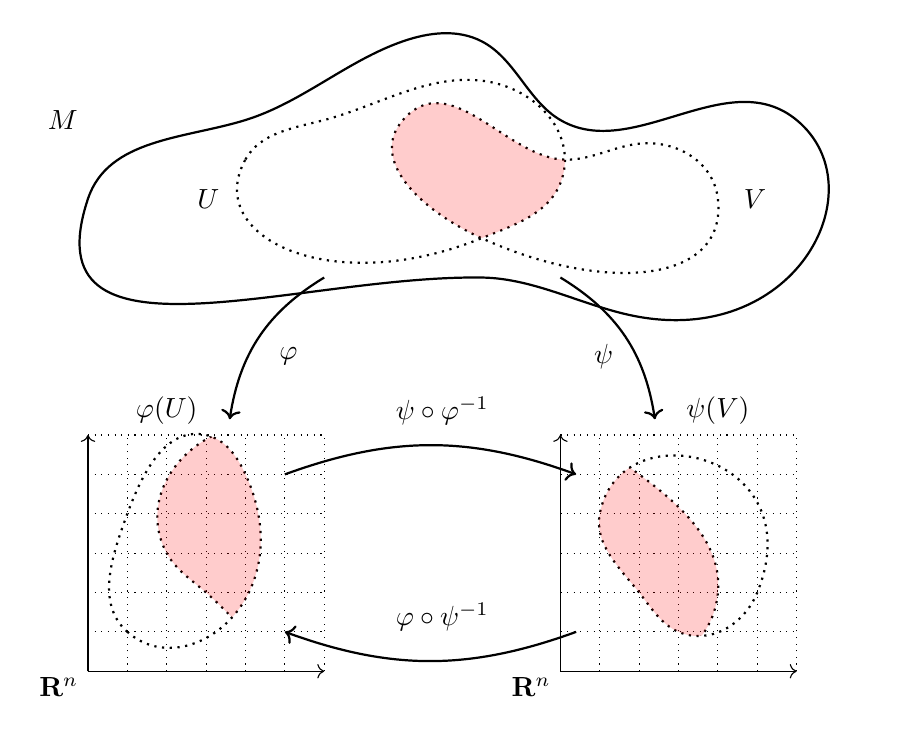
\begin{tikzpicture}
  \draw[step = 0.5, thin, dotted] (-3,-3) grid (0,0) node[left] at (-3,-3.2) {$\mathbf{R}^{n}$};
  \draw[->] (-3,-3) -- (0,-3);
  \draw[->] (-3,-3) -- (-3,0);

  \draw[step = 0.5, thin, dotted] (3,-3) grid (6,0) node[left] at (3,-3.2) {$\mathbf{R}^{n}$};
  \draw[->] (3,-3) -- (6,-3);
  \draw[->] (3,-3) -- (3,0);

  \draw[thick] (-3,3) to[closed,curve through = {(-1,4) (1,5) (2,5) (3,4) (6,4) (4,1.5)}] (2,2) node[left] at (-3,4) {$M$};
  
  \draw[thick, dotted] (-1,3.5) to[closed,curve through = {(0,4) (2,4.5) (3,3.2)}] (2,2.5) node[left] at (-1.2,3) {$U$}; 


  \draw[thick, dotted] (1,4) to[closed,curve through = {(3,3.5) (4,3.7) (5,3)}] (2,2.5) node[right] at (5.2,3) {$V$};

  \begin{scope}
    \clip (-1,3.5) to[closed,curve through = {(0,4) (2,4.5) (3,3.2)}] (2,2.5);
    \fill[red, opacity = 0.2] (1,4) to[closed,curve through = {(3,3.5) (4,3.7) (5,3)}] (2,2.5);
  \end{scope}

  %\fill (2,3) circle (0.5mm);

  \draw[thick,dotted] (-2.5,-2.5) to[closed,curve through = {(-2.5,-1) (-1.5,0)}] (-1,-0.5) node[above] at (-2,0) {$\varphi(U)$};

  \draw[thick,dotted] (4,-2) to[closed,curve through = {(3.5,-1) (5.5,-2)}] (4.5,-2.5) node[above] at (5,0) {$\psi(V)$};

  % \draw[thick,dotted] (0,0) to[closed,curve through = {(-2,-1.5) (-1.5,-2)}] (0,-3);

  \begin{scope}
    \clip (-2.5,-2.5) to[closed,curve through = {(-2.5,-1) (-1.5,0)}] (-1,-0.5);
    \draw[thick,dotted] (0,0) to[closed,curve through = {(-2,-1.5) (-1.5,-2)}] (0,-3);
    \fill[red, opacity = 0.2] (0,0) to[closed,curve through = {(-2,-1.5) (-1.5,-2)}] (0,-3);
  \end{scope}

  %\draw[thick,dotted] (2.5,0) to[closed,curve through = {(4,-0.5) (5,-2)}] (3,-3);

  \begin{scope}
    \clip (4,-2) to[closed,curve through = {(3.5,-1) (5.5,-2)}] (4.5,-2.5);
    \draw[thick,dotted] (2.5,0) to[closed,curve through = {(4,-0.5) (5,-2)}] (3,-3);
    \fill[red, opacity = 0.2] (2.5,0) to[closed,curve through = {(4,-0.5) (5,-2)}] (3,-3);
  \end{scope}

  \draw[->,thick] (0,2) to[bend right = 25] (-1.2,0.2) node[right] at (-0.7,1) {$\varphi$};

  \draw[->,thick] (3,2) to[bend left = 25] (4.2,0.2) node[left] at (3.8,1) {$\psi$};

  \draw[->,thick] (-0.5,-0.5) to[bend left = 20] (3.2,-0.5) node[above] at (1.5,0) {$\psi\circ \varphi^{-1}$};

  \draw[<-,thick] (-0.5,-2.5) to[bend right = 20] (3.2,-2.5) node[below] at (1.5,-2) {$\varphi \circ \psi^{-1}$};
\end{tikzpicture}
\end{center}

\Definition{
  位相多様体$M$の\index{あとらす@アトラス}\index{atlas}
  \textbf{アトラス(atlas)}とは,$M$を被覆するチャートの族のことである.
  アトラス$\mathcal{A}$が\index{なめらか@滑らか!なあとらす@なアトラス}\index{smooth! atlas}
  \textbf{滑らかなアトラス(smooth atlas)}とは
  $\mathcal{A}$の任意の二つのチャートがsmoothly compatibleであるときをいう.
}
この滑らかなアトラスが位相多様体に微分構造(smooth structure)を定義するのだが,
同じ位相多様体に異なる微分構造が入った時いつ同一視するか?という問題がある.
例えば,$\mathbf{R}^{n}$のアトラス
\begin{align*}
  &\mathcal{A}_{1} = \{(\mathbf{R}^{n},\text{id}_{\mathbf{R}^{n}})\}\\
  &\mathcal{A}_{2} = \{(B(x;1),\text{id}_{B(x;1)})\}_{x\in \mathbf{R}^{n}}
\end{align*}
ここで$x\in \mathbf{R}^{n}$と正の実数$r$に対して
\begin{equation*}
  B(x;r) \defi \{y\in \mathbf{R}^{n}\mid d(x,y) < r\}
\end{equation*}
$d:\mathbf{R}^{n}\times \mathbf{R}^{n} \to \mathbf{R}_{\geq 0}$はユークリッド空間の通常の距離関数である.
これらは違う滑らかなアトラスだが,関数$f:\mathbf{R}^{n} \to \mathbf{R}$\\ \\
後で加筆する.

\Definition{
  滑らかなアトラス$\mathcal{A}$が\textbf{極大(maximal)}とは,$\mathcal{A}$を真に包含する
  滑らかなアトラスが存在しない時をいう.
}

\Definition{
  位相多様体$M$の極大な滑らかなアトラスを\index{びぶんこうぞう@微分構造}\index{smooth! structure}
  \textbf{微分構造(smooth structure)}という.\index{なめらか@滑らか!なたようたい@な多様体}\index{smooth! manifold}
  \textbf{滑らかな多様体(smooth manifold)}とは位相多様体とその微分構造の組$(M,\mathcal{A})$
  のことをいう.このとき微分構造が明らかなときは単に$M$は滑らかな多様体という.
  滑らかな多様体は,また\textbf{可微分多様体(differentiable manifold)}
  という.
}


\Proposition{
  位相多様体$M$に対して以下が成り立つ.
  \begin{itemize}
    \item[(1)] 任意の$M$の滑らかなアトラス$\mathcal{A}$に対して$\mathcal{A}$を含む極大な滑らかなアトラスが唯一存在する.これを\textbf{$\mathcal{A}$から決まる微分構造(smooth structure determined by $\mathcal{A}$)}という.
    \item[(2)] $M$の二つの滑らかなアトラスが同じ微分構造を決めるということはそれらの合併が滑らかなアトラスになることと必要十分である. 
  \end{itemize}
}{
  $\mathcal{A}$を$M$の滑らかなアトラス,$\overline{\mathcal{A}}$を
  $\mathcal{A}$の任意のチャートとsmoothly compatibleなチャートの集合とする.
  このとき$\overline{\mathcal{A}}$が滑らかなアトラスであることを示そう.
  つまり任意の$\overline{\mathcal{A}}$の二つのチャートがsmoothly compatible
  であることを示せば良い.つまり定義から$(U,\varphi),(V,\psi)\in \overline{\mathcal{A}}$
  に対して
  \begin{equation*}
    \psi\circ \varphi^{-1}:\varphi(U\cap V) \to \psi(U\cap V)
  \end{equation*}
  が滑らかであることを確認すればよい.$\varphi(p) \in \varphi(U\cap V)$
  をとる.アトラス$\mathcal{A}$は$M$を被覆するので$p\in W$なる$(W,\theta) \in \mathcal{A}$
  を取れる.$\overline{A}$の任意のチャートは$(W,\theta)$とsmoothly compatible
  なので,$\theta\circ \varphi^{-1}$,$\psi \circ \theta^{-1}$は滑らかである.
  よって,$p\in U\cap V \cap W$に対して,
  \begin{equation*}
    \psi \circ \varphi^{-1} = (\psi \circ \theta^{-1})\circ (\theta \circ \varphi^{-1})
  \end{equation*}
  は点$\varphi(p)$近傍で滑らかである.今$\varphi(p)\in \varphi(U\cap V)$は任意なので
  $\psi\circ \varphi^{-1}$は$\varphi(U\cap V)$の任意の点の近傍で滑らかである.
  よって$\overline{\mathcal{A}}$は滑らかなアトラスである.\\
  あとは,極大であることを確認すれば良い.$\overline{\mathcal{A}}\subset \mathcal{B}$なる滑らかなアトラス$\mathcal{B}$を取ると,
  $\mathcal{A} \subset \mathcal{B}$と定義から$\mathcal{B}$の任意のチャートは
  $\mathcal{A}$の任意のチャートとsmoothly compatibleである.従って$\overline{\mathcal{A}}$の取り方から逆の包含関係も分かる.又,同様に,唯一性もわかる.
}

smoothly compatibleを弱めて,アトラスの任意の二つのチャートの座標変換写像が$C^{k}$級
で,極大なとき\textbf{$C^{k}$構造($C^{k}$ structure)}という.同様に,座標変換写像が,
実解析的(real-analytic)なとき,\textbf{実解析的構造(real-analytic structure)}
または\textbf{$C^{\omega}$構造($C^{\omega}$ structure)}という.
もし次元が$2m$なら$\mathbf{R}^{2m}$と$\mathbf{C}^{m}$とを同一視して,また,
座標変換写像を複素解析的(正則関数)とすることで,\textbf{複素解析的構造(complex-analytic structure)}が定義できる.


\Definition{
  可微分多様体$M$のチャート$(U,\varphi)$が$M$の微分構造(滑らかなアトラス)に含まれているとき\index{なめらか@滑らか!なちゃーと@なチャート}\index{smooth! chart}
  \textbf{滑らかなチャート(smooth chart)}という.また,$\varphi$を
  \index{なめらか@滑らか!なざひょうしゃぞう@な座標写像}\index{smooth! coordinate map}
  \textbf{滑らかな座標写像(smooth coordinate map)}という.
  \index{なめらか@滑らか!なざひょうきゅう@な座標球}\index{smooth! coordinate ball}
  \textbf{滑らかな座標球(smooth coordinate ball)}とは,滑らかのチャート$(U,\varphi)$
  であり,$\varphi(U)$がユークリッド空間の球であるときをいう.同様に
  \index{なめらか@滑らか!なざひょうりっぽうたい@な座標立方体}\index{smooth! coordinate cube}
  \textbf{滑らかな座標立方体(smooth coordinate cube)}が定義される.
}

\Definition{
  $B$が\index{せいそくざひょうきゅう@正則座標球}\index{regular coordinate ball}
  \textbf{正則座標球(regular coordinate ball)}とは$\overline{B}\subset B'$なる
  滑らかな座標球$B'$が存在し,滑らかな座標写像$\varphi:B'\to \mathbf{R}^{n}$が
  ある$r < r'$なる正の実数$r,r'$に対して
  \begin{equation*}
    \varphi(B) = B(0;r),\ \varphi(\overline{B}) = \overline{B(0;r)},\ \varphi(B') = B(0;r')
  \end{equation*}
  となるときをいう.
}

\Proposition{
  任意の可微分多様体は正則座標球の加算開基を持つ.
}{}





\Section{Smooth Maps}

\Definition{
  $n$次元可微分多様体$M$,$k\in \mathbf{Z}_{> 0}$に対して$f:M\to \mathbf{R}^{k}$
  が\index{なめらか@なめらか!なかんすう@なかんすう}\index{smooth! function}
  \textbf{滑らかな関数(smooth function)}とは,任意の点$p\in M$に対して,
  それを含む滑らかなチャート$(U,\varphi)$があって
  \begin{equation*}
    f\circ \varphi^{-1}:\varphi(U) \to \mathbf{R}^{k}
  \end{equation*}
  が滑らかなときをいう.
  \begin{equation*}
    C^{\infty}(M) \defi \{f:M\to \mathbf{R} \mid f \text{ is smooth}\}
  \end{equation*}
  と置く.これは$\mathbf{R}$上のベクトル空間である.
}

\Definition{
  $M,N$を可微分多様体とする.このとき$F:M\to N$が\index{なめらか@滑らか!なしゃぞう@な写像}\index{smooth! map}
  \textbf{滑らかな写像(smooth map)}とは任意の点$p\in M$に対して,それを含む
  滑らかなチャート$(U,\varphi)$と$F(p)$を含む滑らかなチャート$(V,\psi)$があって,
  $F(U)\subset V$で,
  \begin{equation*}
    \psi \circ F \circ \varphi^{-1}:\varphi(U) \to \psi(V)
  \end{equation*}
  が滑らかなときをいう.
}

\Proposition{
  滑らかな写像は連続である.
}{
  $M,N$を可微分多様体として,$F:M\to N$は$p\in M$で滑らかとする.
  つまり,$p$を含む滑らかなチャート$(U,\varphi)$と$F(p)$を含む滑らかなチャート$(V,\psi)$が$F(U)\subset V$で,
  \begin{equation*}
    \psi \circ F\circ \varphi^{-1} : \varphi(U) \to \psi(V)
  \end{equation*}
  が滑らかであるようにとれる.よって$\psi \circ F\circ \varphi^{-1}$は連続で,
  $\varphi :U \to \varphi(U)$,$\psi:V\to \psi(V)$は同相写像なので,
  \begin{equation*}
    F|_{U} = \psi^{-1} \circ (\psi \circ F\circ \varphi^{-1}) \circ \varphi : U\to V
  \end{equation*}
  は,連続である.よって任意の点の近傍で$F$は連続なので,$M$で連続である.
}

\Proposition{
  可微分多様体$M,N,P$に対して以下が成り立つ.
  \begin{itemize}
    \item[(1)] 任意の定数写像$c:M\to N$は滑らかである.
    \item[(2)] 恒等写像$\text{id}_{M}:M\to M$は滑らかである.
    \item[(3)] 開部分多様体$U\subset M$に対して包含写像$U \hookrightarrow M$は滑らかである.
    \item[(4)] $F:M\to N$,$G:N\to P$が滑らかなら,$G\circ F:M\to P$は滑らかである.   
  \end{itemize}
}{
  \Claim{(1)}\\
  $p\in M$を含む滑らかなチャート$(U,\varphi)$と,$c(p) = c$を含む滑らかなチャート$(V,\psi)$は$c(U) = \{c\} \subset V$である.また任意の$x\in \varphi(U)$に対して
  \begin{equation*}
    (\psi\circ c \circ \varphi^{-1})(x) = \psi(c)
  \end{equation*}
  で,$\psi$は$C^{\infty}$なので,定数写像$c$は滑らかである.\\
  \Claim{(2)}\\
  (1)と同じようにチャート$(U,\varphi)$,$(V,\psi)$を取る.ただし$\text{id}_{M}(U)=U\subset V$となるように取る.すると
  \begin{equation*}
    \psi \circ \text{id}_{M} \circ \varphi^{-1} = \psi \circ \varphi^{-1}
  \end{equation*}
  これは座標変換写像であり,定義から$C^{\infty}$である.よって$\text{id}_{M}$は滑らかである.\\
  \Claim{(3)}\\
  部分多様体の定義をかけ!!\\
  \Claim{(4)}\\
  $p\in M$を含む滑らかなチャート$(U,\varphi)$と,$F(p)$を含む滑らかなチャート$(V,\psi)$で$F(U)\subset V$が成り立つように取る.また,$G(F(p))$を含む滑らかなチャート$(W,\theta)$で,$G(V)\subset W$が成り立つように取る. 
  (つまり,$G(F(U))\subset W$が成り立つ.)よって,$F,G$の滑らかさから,
  \begin{align*}
    \psi \circ F \circ \varphi^{-1}:\varphi(U) \to \psi(V)\\
    \theta \circ G \circ \psi^{-1}:\psi(V) \to \theta(W)
  \end{align*}
  は滑らかである.よって,
  \begin{equation*}
    \theta \circ (G \circ F) \circ \varphi^{-1} = (\theta \circ G \circ \psi^{-1}) \circ (\psi \circ F \circ \varphi^{-1})
  \end{equation*}
  は滑らかである.
}


\Section{Tangent Space}

まず,可微分多様体$M$と$p\in M$に対して,$p$近傍で定義されている$C^{\infty}$実数値関数$f,g$に対して二項関係$\sim$を
\begin{equation*}
  f\sim g \defi p\in \exists W:\text{open}, f|_{W} = g|_{W}
\end{equation*}
と定義する.すると,これは同値関係である.この同値関係で$p$近傍で定義されている$C^{\infty}$実数値関数の集合を割った集合を$C^{\infty}_{p}(M)$と書く.
\begin{equation*}
  C^{\infty}_{p}(M) \defi \{f:U\to \mathbf{R}\mid p\in U:\text{open}\}/\sim
\end{equation*}
これは,関数の和と積で$\mathbf{R}$多元環を成す.\\
$C^{\infty}_{p}(M)$の元は本来$C^{\infty}$関数$f:U\to \mathbf{R}$を用いて,
\begin{equation*}
  [f] \in C^{\infty}_{p}(M)
\end{equation*}
などと書かれるべきだが,面倒なのでこれを$f$と書いてしまおう.\\
さて,早速接空間(tangent space)を定義していこう.
\Definition{
  可微分多様体$M$の\index{どうぶん@導分}\index{derivation}
  \textbf{点$p$における導分(derivation at $p$)}とは,線形写像$D:C^{\infty}_{p}(M) \to \mathbf{R}$であって,
  \begin{equation*}
    D(fg) = D(f)g(p) + f(p)D(g)
  \end{equation*}
  を満たすものとして定義する.また,$M$の点$p$における\index{せつべくとる@接ベクトル}\index{tangent vector}
  \textbf{接ベクトル(tangent vector)}とは,点$p$における導分のことである.\\
  点$p$における接ベクトル全体はベクトル空間を成す.これを$T_{p}(M)$または,$T_{p}M$と書いて,\index{せつくうかん@接空間}\index{tangent space}\textbf{点$p$における$M$の接空間(tangent space to $M$ at $p$)}という.
}



\subsection{differential}

\Definition{
  可微分多様体$M,N$の間の$C^{\infty}$写像$F:M\to N$を取る.各点$p\in M$に対して
  $F$の\index{びぶん@微分}\index{differential}
  \textbf{点$p$における微分(differential at $p$)}と呼ばれる接空間の間の線型写像
  \begin{equation*}
    dF:T_{p}M \to T_{F(p)}N
  \end{equation*}
  が,$X_{p}\in T_{p}M$に対して$dF(X_{p})$は
  \begin{equation*}
    dF(X_{p})(f) \defi X_{p}(f\circ F)\qquad (f\in C^{\infty}_{F(p)}(N))
  \end{equation*}
  なる接ベクトルである.
}

\Example{
  $M$を可微分多様体として滑らかな関数$f:M\to \mathbf{R}$の点$p$における
  微分$df:T_{p}M\to T_{p}\mathbf{R} \cong \mathbf{R}$は
  \begin{equation*}
    C^{\infty}_{f(p)}(\mathbf{R}) = 
  \end{equation*}
  $X_{p} \in T_{p}M$に対して
  \begin{equation*}
    df(X_{p})(g) = X_{p}(f \circ g)
  \end{equation*}
}{}

\Remark{
  どの点における微分であるかを明確にするために$dF$の代わりに$dF_{p}$と書くことがある.
}{}

滑らかな写像$F:M\to N$,$G:N\to P$と点$p\in M$に対して線型写像
\[
  \xymatrix{
    T_{p}M \ar@/^25pt/@{>}[rr]^{dG_{F(p)}\circ dF_{p}} \ar@/_25pt/@{>}[rr]_{d(G\circ F)_{p}} \ar[r]^{dF_{p}}& T_{F(p)}N \ar[r]^{dG_{F(p)}} &T_{G(F(p))}
  }
\]

が定義できる.これらは等しい.
\Theorem{
  $F:M\to N$,$G:N\to P$を可微分多様体の間の滑らかな写像とする.このとき$p\in M$ならば
  \begin{equation*}
    d(G\circ F)_{p} = dG_{F(p)}\circ dF_{p}
  \end{equation*}
  が成り立つ.
}{
  $X_{p}\in T_{p}M$を取る.$f\in C^{\infty}_{G(F(p))}(P)$に対して,
  \begin{equation*}
    d(G\circ F)(X_{p})(f) = X_{p}(f\circ (G\circ F))
  \end{equation*}
  で,また
  \begin{equation*}
    (dG\circ dF)(X_{p})(f) = dG(dF(X_{p}))(f) = dF(X_{p})(f\circ G) = X_{p}(f\circ G\circ F)
  \end{equation*}
}

\Corollary{
  $F:M\to N$が可微分多様体の間の微分同相写像とする.このとき$dF_p:T_{p}M \to T_{F(p)}N$は同型写像である.
}{}

\Corollary{
  開集合$U\subset \mathbf{R}^{n}$が開集合$V\subset \mathbf{R}^{m}$と微分同相ならば,$n=m$である.
}{
  $F:U\to V$を微分同相写像とする.このとき先程の系より,
  \begin{equation*}
    dF_{p} : T_{p}U \to T_{F(p)}V
  \end{equation*}
  は同型写像である.また,$T_{p}U = T_{p}\mathbf{R}^{n} \simeq \mathbf{R}^{n}$
  ,$T_{F(p)}V = T_{F(p)}\mathbf{R}^{m} \simeq \mathbf{R}^{m}$より,$n=m$を得る.
}

$n$次元可微分多様体$M$の点$p$を含む滑らかなチャート$(U,\varphi = (x^{1},\dots ,x^{n}))$をとる.このとき$\varphi:U\to \varphi(U)$は微分同相写像なので,
\begin{equation*}
  d\varphi_{p}:T_{p}M\to T_{\varphi(p)}\mathbf{R}^{n}
\end{equation*}
は同型写像である.特に$T_{p}M$の次元は$n$である.

\Proposition{
  $(U,\varphi = (x^{1},\dots ,x^{n}))$を$n$次元可微分多様体$M$の点$p$を含む滑らかなチャートとする.このとき
  \begin{equation*}
    d\varphi_{p}\left( \left. \frac{\partial}{\partial x^{i}} \right|_{p}\right) = \left. \frac{\partial}{\partial r^{i}} \right|_{\varphi(p)}
  \end{equation*}
}{
  $f\in C^{\infty}_{\varphi(p)}(\mathbf{R}^{n})$に対して
  \begin{align*}
    d\varphi_{p}\left( \left. \frac{\partial}{\partial x^{i}} \right|_{p}\right)f
    &= \left. \frac{\partial}{\partial x^{i}} \right|_{p} (f\circ \varphi)\\
    &= \left. \frac{\partial}{\partial r^{i}} \right|_{\varphi(p)} (f\circ \varphi \circ \varphi^{-1})\\
    &= \left. \frac{\partial}{\partial r^{i}} \right|_{\varphi(p)} f
  \end{align*}
}

\Proposition{
  点$p\in M$を含む滑らかなチャート$(U,\varphi = (x^{1},\dots ,x^{n}))$を取る.すると接空間$T_{p}M$は基底
  \begin{equation*}
    \left. \frac{\partial}{\partial x^{1}} \right|_{p},\dots ,\left. \frac{\partial}{\partial x^{n}} \right|_{p}
  \end{equation*}
  を持つ.
}{
  ベクトル空間の同型写像は基底を基底に移す.先程の命題より,同型写像
  \begin{equation*}
    d\varphi_{p}:T_{p}M \to T_{\varphi(p)}\mathbf{R}^{n}
  \end{equation*}
  は$\partial/\partial x^{i}|_{p}$を$\partial/\partial r^{i} |_{\varphi(p)}$に移すが,
  $\partial/\partial r^{i}|_{\varphi(p)}$は$T_{\varphi(p)}\mathbf{R}^{n}$の基底なので,$\partial/\partial x^{i}|_{p}$は$T_{p}M$の基底である.
}



\Section{Vector Field}
多様体$M$においてそのすべての点で時間$t$に応じて運動し
$M$の上に滑らかな流れが生じている状態を考えてみよう.

\begin{center}
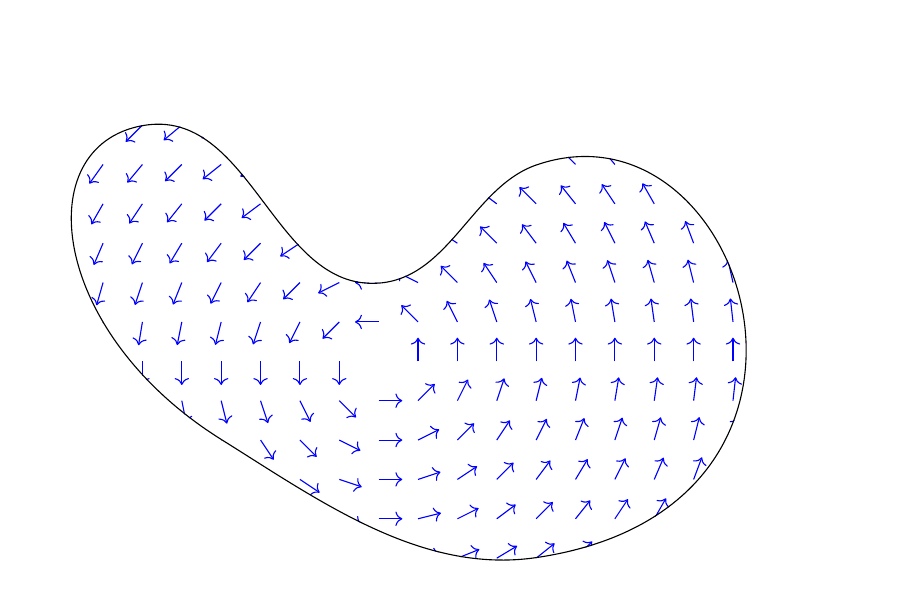
\begin{tikzpicture}
  \clip (-3,3) to[closed, curve through = {(-2,-1) (2,-2.5) (2,2.5)}] (0,1) node[left] at (-3,4) {$M$};

% ベクトル場の描画
\foreach \x in {-4,-3.5,...,5} {
    \foreach \y in {-4,-3.5,...,4} {
        % ベクトルの方向と長さを定義
        \pgfmathsetmacro{\vx}{-\y}
        \pgfmathsetmacro{\vy}{\x}
        \pgfmathsetmacro{\magnitude}{sqrt(\vx*\vx+\vy*\vy)}
        % ゼロ除算を防ぐ
        \ifdim \magnitude pt > 0pt
            \pgfmathsetmacro{\scale}{0.3/\magnitude}
        \else
            \pgfmathsetmacro{\scale}{0} % 矢印を描画しない
        \fi
        % 矢印の描画(\scaleがゼロの場合はスキップ)
        \ifdim \scale pt > 0pt
            \draw[->, blue] (\x, \y) -- ++(\scale*\vx, \scale*\vy);
        \fi
    }
}




\draw[thick] (-3,3) to[closed, curve through = {(-2,-1) (2,-2.5) (2,2.5)}] (0,1) node[left] at (-3,4) {$M$};



\end{tikzpicture}
\end{center}




\Definition{
多様体$M$において,各実数$t$に対して滑らかな写像$\varphi_{t}:M \to M$
が与えられ,次を満たすとき$\{\varphi_{t}\}$を$M$の\textbf{1パラメーター変換群}という.
\begin{itemize}
  \item[(1)] $\varphi_{s}\circ \varphi_{t} = \varphi_{s+t},\quad \varphi_{0} = 1_{M}$
  \item[(2)] 写像$\mathbf{R}\times M\to M;(t,x)\mapsto \varphi_{t}(x)$は滑らかである. 
\end{itemize}
}
曲線の接ベクトルを考えれば
\begin{equation}
  X_{x}f = \lim_{t\to 0}\frac{f(\varphi_{t}(x)) - f(x)}{t}
\end{equation}


\Section{Vector Bundle}

底空間を位相空間とする場合でベクトルバンドルを定義しよう.

\Definition{
  $X$を位相空間とする.$X$上の\textbf{ベクトル空間の族(family of vector spaces)}とは,位相空間$E$に
  \begin{itemize}
    \item[(1)] 連続写像$p:E\to X$
    \item[(2)] $x\in X$に対するそれぞれの
    \begin{equation*}
      E_{x} = p^{-1}(\{x\})
    \end{equation*}
    が有限次元ベクトル空間であり,$E$から誘導される位相と整合的である.
  \end{itemize}
  を満たすものをいう.
}
族$p:E\to X$の\textbf{切断(section)}とは連続写像$s:X\to E$で,$p\circ s = 1$となるときをいう.




\Section{Diffrential Form}

$K$を標数$0$の体,$F$を$K$多元環,$V$は$F$加群とする.\\
とても大切なのは$K=\mathbf{R},\mathbf{C}$の場合である.
\Example{
  $F = K$のとき$V$は$K$上のベクトル空間である.
}{}

\Example{
  $M$を可微分多様体とすれば$C^{\infty}_{p}(M)$は$\mathbf{R}$多元環で,
  $M$上で定義されたベクトル場すべてのつくるアーベル群$\mathcal{X}$は$C^{\infty}_{p}(M)$加群である.
}{}

\Definition{
  $F=K$として$V$を$K$上の$n$次元ベクトル空間とする.写像
  \begin{equation*}
    \phi : \underbrace{V\times \dots \times V}_{\text{$k$個}} \to K
  \end{equation*}
  が\textbf{$k$重線型写像(えいご)}
  とは各変数に関して線型であることをいう.つまり$i = 1,\dots,k$に対して
  \begin{equation*}
    \phi(v_{1},\dots,\alpha v_{i} + \beta w_{i},\dots,v_{k}) = \alpha\phi(v_{1},\dots, v_{i},\dots,v_{k}) + \beta \phi(v_{1},\dots, w_{i},\dots, v_{k})
  \end{equation*}
  が成り立つときをいう.
}

\Definition{
  $p\in \mathbf{Z}_{\geq 0}$に対して$F$加群$V$上の\textbf{$p$次交代形式($p$-th alternating form)}
  
}


\Proposition{
  $\phi \in \Lambda^{k}V^{*}, \psi \in \Lambda^{l}V^{*}$とするとき,次が成り立つ.
  \begin{enumerate}
    \item $\phi \wedge \psi = (-1)^{kl}\psi \wedge \psi \in \Lambda^{k+l}V^{*}$
    \item $v_{1},\dots,v_{k+l} \in V$とする.このとき,
    \begin{equation*}
      (\phi \wedge \psi)(v_{1},\dots,v_{k+l}) = \frac{1}{k!l!}\sum_{\sigma \in S_{k+l}}\text{sgn}(\sigma)\phi(v_{\sigma(1)},\dots,v_{\sigma(k)})\psi(v_{\sigma(k+1)},\dots,v_{\sigma(k+l)})
    \end{equation*}
  \end{enumerate}
}{}

\chapter{Complex Analysis}

\Section{Holomorphic Function}
\noindent
複素数$z = x + iy\in \mathbf{C}$に対して$|z|$を
\begin{equation}
  |z| \defi \sqrt{x^{2} + y^{2}}
\end{equation}
と定義する.定義とコーシー・シュワルツの不等式から$z,w\in \mathbf{C}$に対して
\begin{align}
  &|z| = 0 \Leftrightarrow z = 0\\
  &|zw| = |z||w|\\
  &|z + w| \leq |z| + |w|\qquad (三角不等式)
\end{align}
が成り立つ.三角不等式より
\begin{equation}
  ||z|-|w|| \leq |z - w|
\end{equation}
が成り立つ.実際
\begin{align*}
  |z| = |z - w + w| \leq |z - w| + |w| 
\end{align*}
より$|z| - |w| \leq |z - w|$で,対称性から$-(|z| - |w|) \leq |z-w|$より式(B.5)を
得る.\\
集合$\Omega \subset \mathbf{C}$上で定義された関数
$f:\Omega \subset \mathbf{C} \to \mathbf{C}$が$z_{0}\in \Omega$で
\index{れんぞく@連続}\index{continuous}\textbf{連続(continuous)}とは,
任意の$\varepsilon \in \mathbf{R}_{>0}$に対して,ある$\delta \in \mathbf{R}_{>0}$
が存在して
\begin{equation}
  |z - z_{0}| < \delta \Rightarrow |f(z) - f(z_{0})| < \varepsilon
\end{equation}
を満たすことである.
\footnote{ただし,$\delta$を十分小さく取る.具体的には$z\in \Omega$となる程度}
これは,$\Omega$内の点列$(z_{n})_{n}$で$z_{n} \to z_{0}\ (n \to \infty)$
なる任意の点列に対して,
\begin{equation}
  \lim_{n \to \infty}f(z_{n}) = f(z_{0})
\end{equation}
が成り立つことと同値である.
$f$が$\Omega$上で連続とは$\Omega$の任意の点で連続なときを言う.\\
$f$が連続ならば実数値関数$|f|$も連続であることがわかる.実際(B.5)より
\begin{equation}
  ||f(z)| - |f(z_{0})|| \leq |f(z) - f(z_{0})|
\end{equation}
なのでよい.\\
$f$が点$z_{0}\in \Omega$で最大値をとるとは,
\begin{equation*}
  |f(z)| \leq |f(z_{0})| \qquad (z\in \Omega)
\end{equation*}
を満たすことである.同様に最小値も定義される.

\Theorem{
  コンパクト集合$\Omega$上の連続関数は有界で,$\Omega$において最大値と最小値をとる.
}{}

証明は省く.

\Definition{
  $\Omega\subset \mathbf{C}$を開集合とし,$f:\Omega \to \mathbf{C}$が$z_{0}\in \Omega$
  で\index{せいそく@正則}\index{regular}\index{non-singular}
  \textbf{正則(regular/non-singular)}であるとは,
  \begin{equation}
    \frac{f(z+h) - f(z)}{h}
  \end{equation}
  が$h\to 0$のときに極限を持つことである.ただし,(B.9)が定義されるために,
  $h\in \mathbf{C}$をゼロでない複素数で$|h|$を十分小さく$z+h\in \Omega$
  となるように取る.この極限が存在する場合$f'(z_{0})$と書いて
  $f$の$z_{0}$における微分という.ただし,この極限において$h$はすべての方向から
  $0$に近づくような複素数であることに注意.\\
  $f$が$\Omega$で正則とは,$f$が$\Omega$の任意の点で正則であるときを言う.\\
  $\Omega$が開でないときは,$\Omega$を含むある開集合上で正則で$f$が正則である
  ということにする.$f$が$\mathbf{C}$で正則のとき$f$を
  \index{せいかんすう@整関数}\index{entire function}
  \textbf{整関数}という.
}

\Proposition{
  $f,g$を$\Omega$上の正則関数とする.このとき以下が成り立つ.
  \begin{itemize}
    \item $f+g$は$\Omega$上で正則で,$(f + g)' = f' + g'$である.
    \item $fg$は$\Omega$上で正則で,$(fg)' = f'g + fg'$である.
    \item $g(z_{0}) \neq 0$ならば$f/g$は$z_{0}$で正則で,
    \begin{equation*}
      \left( \frac{f}{g} \right)' = \frac{f'g - fg'}{g^{2}}
    \end{equation*}
    \item もし$f:\Omega \to U,g:U\to \mathbf{C}$が正則なら,
    \begin{equation*}
      (g\circ f)'(z) = g'(f(z))f'(z)\qquad (z \in \Omega)
    \end{equation*}
    が成り立つ.
  \end{itemize}
}{}

\Example{
  $f(z) = z$は正則で,$f'(z) = 1$である.よってProp:\ref{Prop:B.1.2}より,
  多項式
  \begin{equation*}
    p(z) = \sum_{i=0}^{n}a_{i}x^{i}
  \end{equation*}
  は$\mathbf{C}$で正則で,
  \begin{equation*}
    p'(z) = \sum_{i=1}^{n}i a_{i}x^{i-1}
  \end{equation*}
  である.
}{}

\Example{
  $f(z) = \bar{z}$は正則ではない.
}{}

\noindent
(B.9)の$h$が実数の場合の極限を考えよう.特に$h = h_{1} + ih_{2}$として$h_{2} = 0$
の場合を考えよう.このとき$f(z) = f(x,y)$と書くことにすると,
\begin{equation}
  f'(z) = \lim_{h_{1} \to 0}\frac{f(x + h_{1},y) - f(x,y)}{h_{1}} = \frac{\partial f}{\partial x}(z)
\end{equation}
次に$h_{1} = 0$として考えると,
\begin{equation}
  f'(z) = \lim_{h_{2} \to 0}\frac{f(x,y + h_{2}) - f(x,y)}{ih_{2}} = \frac{1}{i}\frac{\partial f}{\partial y}(z)
\end{equation}
よって,$f$が正則なら
\begin{equation}
  \frac{\partial f}{\partial x} = \frac{1}{i}\frac{\partial f}{\partial y}
\end{equation}
が成り立つ.$f = u + iv$とかけば,
\begin{equation}
  \frac{\partial u}{\partial x} = \frac{\partial v}{\partial y},\quad \frac{\partial u}{\partial y} = - \frac{\partial v}{\partial x}
\end{equation}
が成り立つことがわかる.
これらの関係式(B.13)を\index{こーしーりーまんのほうていしき@コーシー・リーマンの方程式}
\index{Cauchy-Riemann equations}
\textbf{コーシー・リーマンの方程式(Cauchy-Riemann equations)}という.
ここで,ウェルティンガーの微分を定義する.
\begin{equation}
  \frac{\partial}{\partial z}\defi \frac{1}{2}\left( \frac{\partial}{\partial x} + \frac{1}{i}\frac{\partial}{\partial y} \right),\quad \frac{\partial}{\partial \bar{z}} \defi \frac{1}{2}\left( \frac{\partial}{\partial x} - \frac{1}{i}\frac{\partial}{\partial y} \right)
\end{equation}

\Proposition{
  $f$が$z_{0}$で正則なら
  \begin{equation}
    \frac{\partial f}{\partial \bar{z}}(z_{0}) = 0 
  \end{equation}
}{
  $f = u + iv$と置くと,
  \begin{align*}
    \frac{\partial f}{\partial \bar{z}} 
    &= \frac{1}{2}\left( \frac{\partial f}{\partial x} - \frac{1}{i}\frac{\partial f}{\partial y} \right)\\
    &= \frac{1}{2}\left( \frac{\partial u}{\partial x} + i\frac{\partial v}{\partial x} - \frac{1}{i}\left( \frac{\partial u}{\partial y} + i\frac{\partial v}{\partial y} \right) \right)\\
    &= \frac{1}{2} \left( \left( \frac{\partial u}{\partial x} - \frac{\partial v}{\partial y} \right) +i\left( \frac{\partial u}{\partial y} + \frac{\partial v}{\partial x} \right)  \right)
  \end{align*}
  よってコーシー・リーマンの方程式と同値である.
}

\Theorem{
  $f=u + iv$を開集合$\Omega$上で定義された複素数値関数とする.もし,$u,v$が
  $C^1$級で,コーシー・リーマンの方程式を満たすならば,$f$は$\Omega$上で正則で,
  $f'(z) = \partial f/\partial z$を満たす.
}{
  \begin{align*}
    u(x + h_{1},y + h_{2}) - u(x,y) = \frac{\partial u}{\partial x}h_{1} + \frac{\partial u}{\partial y}h_{2} + |h|\varepsilon_{1}(h)\\
    v(x + h_{1},y + h_{2}) - v(x,y) = \frac{\partial v}{\partial x}h_{1} + \frac{\partial v}{\partial y}h_{2} + |h|\varepsilon_{2}(h)
  \end{align*}
  で表せる.ただしここで,$h = h_{1} + ih_{2}$が$|h| \to 0$のとき
  $\varepsilon_{i}(h) \to 0$を満たしている.コーシー・リーマンの方程式を用いれば,
  \begin{align*}
    f(x + h) - f(x) 
    &= u(x + h_{1},y + h_{2}) - u(x,y) + i(v(x + h_{1},y + h_{2}) - v(x,y))\\
    &= \frac{\partial u}{\partial x}h_{1} + \frac{\partial u}{\partial y}h_{2} + i\left( \frac{\partial v}{\partial x}h_{1} + \frac{\partial v}{\partial y}h_{2} \right) + |h|\varepsilon(h)\\
    &= \frac{\partial u}{\partial x}h_{1} + \frac{\partial u}{\partial y}h_{2} + i\left( -\frac{\partial u}{\partial y}h_{1} + \frac{\partial u}{\partial x}h_{2} \right) + |h|\varepsilon(h)\\
    &= \left( \frac{\partial u}{\partial x} - i\frac{\partial u}{\partial y} \right)(h_{1} + ih_{2}) + |h|\varepsilon(h)
  \end{align*}
  ただし,$|h| \to 0$のとき$\varepsilon(h) = \varepsilon_{1}(h) + i\varepsilon_{2}(h) \to 0$を満たしている.
  ゆえに$f$は正則で,
  \begin{equation}
    f'(z) = 2\frac{\partial u}{\partial z} = \frac{\partial f}{\partial z}
  \end{equation}
  が成り立つ.
}
\noindent
次に冪級数
\begin{equation}
  \sum_{n = 0}^{\infty}a_{n}z^{n}\qquad (a_{i} \in \mathbf{C})
\end{equation}
について考えよう.(めんどうなので和の範囲を省略して$\sum a_{n}z^{n}$と書くこともある.)
最初に次の定理を証明しよう.
\Theorem{
  冪級数$\sum a_{n}z^{n}$に対して$0\leq R \leq \infty$で,次を満たすものが存在する.
  \begin{itemize}
    \item[(1)] $|z| < R$ならばこの級数は絶対収束する.
    \item[(2)] $R < |z|$ならばこの級数は発散する. 
  \end{itemize}
  ここで$\sum z_{n}$絶対収束するとは$\sum |z_{n}|$が収束するときをいう.\\
  便宜上$1/0 = \infty,1/\infty = 0$とすると,$R$は以下で与えられる.
  \begin{align}
    \frac{1}{R} &= \limsup_{n \to \infty} \sqrt[n]{|a_{n}|}\\
    R &= \lim_{n \to \infty}\left| \frac{a_{n}}{a_{n+1}} \right|
  \end{align}
}{
  後で書く.
}

\Definition{
  上の定理の$R$を冪級数の\index{しゅうそくはんけい@収束半径}\index{radius of convergence}
  \textbf{収束半径(radius of convergence)}といい,領域$|z|<R$を
  \index{しゅうそくえん@収束円}\index{circle of convergence}
  \textbf{収束円(circle of convergence)}という.
}

\Remark{
  収束円の境界$|z| = R$上では収束することも発散することもある.
}{}

\Lemma{
  $0$でない収束半径を持つ冪級数$f(z) = \sum a_{n}z^{n}$は$z = 0$で連続である.
}{
  \begin{equation*}
    f(z) - f(0) = \sum_{n = 1}^{\infty}a_{n}z^{n}
  \end{equation*}
  で,両辺絶対値を取ると
  \begin{equation*}
    | f(z) - f(0) | = \left| \sum_{n = 1}^{\infty}a_{n}z^{n} \right| \leq \sum_{n = 1}^{\infty}|a_{n}z^{n}|
  \end{equation*}
  で,$r$を収束半径未満で$0$より大きい実数とすると,$|z| < r$で冪級数は絶対収束する.
  \begin{equation*}
    | f(z) - f(0) | \leq \sum_{n = 1}^{\infty}|a_{n}|\left| \frac{z}{r}r\right|^{n}
  \end{equation*}
  で
  \begin{equation*}
    \left| \frac{z}{r} \right|^{n} < \frac{|z|}{r}
  \end{equation*}
  なので
  \begin{equation*}
    |f(z) - f(0)| \leq \sum_{n = 1}^{\infty}|a_{n}|\frac{|z|}{r}r^{n} =  C|z|
  \end{equation*}
  ($C$は正の定数)だから$f(z)$は$z = 0$で連続である.
}

\Proposition{
  (冪級数の一意性)
  同じ収束半径を持つ冪級数$\sum a_{n}z^{n},\sum b_{n}z^{n}$が等しい
  \begin{equation*}
    \sum_{n = 0}^{\infty}a_{n}z^{n} = \sum_{n = 0}^{\infty}b_{n}z^{n}
  \end{equation*}
  ならば,任意の$n$に対して$a_{n} = b_{n}$が成り立つ.
}{
  先程の補題から関数
  \begin{equation*}
    f(z) = \sum_{n = 0}^{\infty}a_{n}z^{n},\ g(z) = \sum_{n = 0}^{\infty}b_{n}z^{n} 
  \end{equation*}
  は$z = 0$で連続である.したがって
  \begin{equation*}
    \lim_{z \to 0}f(z) = f(0) = a_{0},\ \lim_{z \to 0}g(z) = g(0) = b_{0}
  \end{equation*}
  だから$a_{0} = b_{0}$を得る.\\
  次に,$N > 0$に対して,$N\geq n$までは$a_{n} = b_{n}$が成り立つとすると,
  \begin{equation*}
    \sum_{n = 0}^{\infty}a_{n}z^{n} = a_{0} + a_{1}z + \cdots + a_{N}z^{N} + \sum_{n = N+1}^{\infty}a_{n}z^{n}
  \end{equation*}
  だから
  \begin{equation*}
    \sum_{n = N + 1}^{\infty}a_{n}z^{n} = \sum_{n = N + 1}^{\infty}b_{n}z^{n}
  \end{equation*}
  を得る.両辺を$z^{N + 1}$で割って同様に$z \to 0$とすると,$a_{N + 1} = b_{N + 1}$を得る.
}

\Theorem{
  冪級数$\sum a_{n}z^{n}$の収束円内の点における微分は級数の項別微分$\sum na_{n}z^{n-1}$で与えられる.
  \begin{equation}
    \frac{\partial}{\partial z} \sum_{n = 0}^{\infty}a_{n}z^{n} = \sum_{n = 0}^{\infty}\frac{\partial }{\partial z}a_{n}z^{n} = \sum_{n = 0}^{\infty}na_{n}z^{n-1}
  \end{equation}
  更に,冪級数は微分しても収束半径は変わらない.
}{
  後で書く.
}

\Corollary{
  冪級数はその収束円内で無限回複素微分可能
}{}




\Proposition{

}{}

最後に開集合$\Omega$上の複素数値関数$f$が$z_{0}\in \Omega$で\index{かいせきてき@解析的}\index{analytic}
\textbf{解析的(analytic)}とは,$z_{0}$を中心として,正の収束半径を持つ冪級数
$\sum a_{n}(z - z_{0})^{n}$があって,$z_{0}$のある近傍内の任意の点$z$において
\begin{equation}
  f(z) = \sum_{n = 0}^{\infty}a_{n}(z - z_{0})^{n}
\end{equation}
が成り立つことである.$f$が$\Omega$内の任意の点で解析的であるとき$f$は$\Omega$上で解析的であるという.



\Section{Line Integral}
\Definition{
  \index{ぱらめとりっくきょくせん@パラメトリック曲線}\index{parametric curve}
  \textbf{パラメトリック曲線(parametric curve)}とは,写像
  $c:[a,b]\subset \mathbf{R} \to \mathbf{C}$のことである.\\
  パラメトリック曲線が\index{なめらか@滑らか}\index{smooth}
  \textbf{滑らか(smooth)}とは,$c'(t)$があって,$[a,b]$上で
  連続であり,そして$t\in [a,b]$に対して$c'(t) \neq 0$を満たすことである.
  ただし,点$t=a,t=b$に対しては$c'(a),c'(b)$を片側極限
  \begin{equation*}
    c'(a) = \lim_{\substack{h\to 0 \\ h > 0}}\frac{c(a + h) - c(a)}{h},\quad 
    c'(a) = \lim_{\substack{h\to 0 \\ h < 0}}\frac{c(b + h) - c(b)}{h}
  \end{equation*}
  で定義する.\\
  パラメトリック曲線が\index{くぶんてきになめらか@区分的に滑らか}\index{piecewise smooth}
  \textbf{区分的に滑らか(piecewise smooth)}とは,$c$が$[a,b]$上で連続で,ある
  区間の分割
  \begin{equation*}
    a = a_{0} < a_{1} < \dots < a_{n} = b
  \end{equation*}
  があって,$c(t)$が各区間$[a_{i},a_{i+1}]$において滑らかになっていることである.
  点$a_{i}$における右側微分と左側微分とは一致しないこともありうる.
}
\noindent
二つのパラメトリック曲線
\begin{equation*}
  c:[a,b] \to \mathbf{C},\quad \bar{c}:[c,d] \to \mathbf{C}
\end{equation*}
が同値とは,全単射な$C^{1}$級関数$t:[a,b] \to [c,d]$があって,$t'(s) > 0$かつ
\begin{equation*}
  \bar{c}(t(s)) = c(s)
\end{equation*}
を満たしていることである.\\
区分的に滑らかな曲線が閉とは始点と終点が一致していることをいう.\\
区分的に滑らかな曲線$c$が,単純とは,$c$が単射なときをいう.ただし,曲線が
閉の場合は始点と終点以外の点で単射なとき単純という.

\Example{
  中心を$z_{0}\in \mathbf{C}$とする半径$r$の円周
  \begin{equation*}
    C_{r}(z_{0}) = \{z\in \mathbf{C}\mid |z-z_{0}| = r\}
  \end{equation*}
  は単純閉曲線で,反時計回りのパラメータ付け
  \begin{equation*}
    c(t) = z_{0} + re^{it}\quad (t\in [0,2\pi])
  \end{equation*}
  を正の向きとしておこう.
}{}
漸く積分の定義にありつける.

\Definition{
  $c:[a,b] \to \mathbf{C}$によりパラメーター付けられた滑らかな曲線$\gamma$と
  $\gamma$上の連続関数$f$が与えられたとき,$\gamma$に沿った$f$の積分または$\gamma$上の積分を
  \begin{equation}
    \int_{\gamma} f(z)dz = \int_{a}^{b}f(c(t))c'(t)dt
  \end{equation}
  により,定義する.この定義が意味を持つには,右辺がパラメーター付けに依らないこと
  を示さなければならない.$\bar{c}:[c,d] \to \mathbf{C}$を同値なパラメータ付けだとする.
  このとき積分の変数変換の公式と連鎖律から
  \begin{equation}
    \int_{a}^{b}f(c(t))c'(t)dt 
    = \int_{a}^{b}f(\bar{c}(t(s)))\bar{c}'(t(s))t'(s)ds
    = \int_{c}^{d}f(\bar{c}(s))\bar{c}'(s)ds
  \end{equation}
  が成り立つ.\\
  $\gamma$は区分的に滑らかなときは,$\gamma$上の$f$の積分は,単に区分的に積分
  した和として定義される.すなわち
  \begin{equation}
    \int_{\gamma}f(z)dz = \sum_{k = 0}^{n-1}\int_{a_{k}}^{a_{k+1}}f(c(t))c'(t)dt
  \end{equation}
  である.滑らかな曲線$\gamma$の長さ$L(\gamma)$は
  \begin{equation}
    L(\gamma) = \int_{a}^{b}|c'(t)|dt
  \end{equation}
  と定義する.
}

\Proposition{
  以下が成立する.
  \begin{itemize}
    \item[(1)] $\alpha,\beta \in \mathbf{C}$に対して,
    \begin{equation}
      \int_{\gamma}(\alpha f(z) + \beta g(z))dz = \alpha\int_{\gamma}f(z)dz + \beta\int_{\gamma}g(z)dz
    \end{equation} 
    \item[(2)] $\gamma^{-}$を$\gamma$と逆に向き付けた曲線のとき
    \begin{equation}
      \int_{\gamma^{-}}f(z)dz = - \int_{\gamma}f(z)dz
    \end{equation}
    \item[(3)]次の不等式が成り立つ.
    \begin{equation}
      \left| \int_{\gamma}f(z)dz \right| \leq \sup_{z\in \gamma}|f(z)|\cdot L(\gamma)
    \end{equation}
  \end{itemize}
}{
  気が向いたら書く.
}

\Theorem{
  $f$が開集合$\Omega$で連続で,かつ原始関数$F$をもち,$\gamma$が始点$w_{1}$,終点$w_{2}$の$\Omega$内の曲線であるとき,
  \begin{equation}
    \int_{\gamma}f(z)dz = F(w_{2}) - F(w_{1})
  \end{equation}
  が成り立つ.
}{
  $\gamma$が滑らかなとき,
  $c:[a,b] \to \mathbf{C}$を$\gamma$のパラメータ付けだとすると,$c(a) = w_{1},c(b) = w_{2}$で
  \begin{align*}
    \int_{\gamma}f(z)dz 
    &= \int_{a}^{b}f(c(t))c'(t)dt\\
    &= \int_{a}^{b}F'(c(t))c'(t)dt\\
    &= \int_{a}^{b}\frac{d}{dt}F(c(t))dt\\
    &= F(c(b)) - F(c(a))
  \end{align*}
  である.$\gamma$が区分的に滑らかなとき,
  \begin{align*}
    \int_{\gamma}f(z)dz 
    &= \sum_{k = 0}^{n-1}\int_{a_{k}}^{a_{k+1}}f(c(t))c'(t)dt\\
    &= \sum_{k = 0}^{n-1}(F(c(a_{k+1})) - F(c(a_{k})))\\
    &= F(c(a_{n})) - F(c(a_{0}))\\
    &= F(c(b)) - F(c(a))
  \end{align*}
  を得る.
}

\Corollary{
  $\gamma$が開集合$\Omega$における閉曲線で,$f$が連続かつ$\Omega$で原始関数をもつなら,
  \begin{equation}
    \int_{\gamma}f(z)dz = 0
  \end{equation}
  である.
}{}

\Example{
  $f(z) = 1/z$は$\mathbf{C}\mysetminus\{0\}$で原始関数を持たない.
}{
  $C$を$c(t) = e^{it}\ (0\leq t \leq 2\pi)$でパラメーター付けられた単位円周とすると,
  \begin{equation}
    \int_{C}f(z)dz = \int_{0}^{2\pi}\frac{1}{e^{it}}ie^{it}dt = 2\pi i \neq 0
  \end{equation}
  だからである.
}

\Corollary{
  $f$が領域$\Omega$で正則で,$f' = 0$なら$f$は定数である.
}{
  点$w_{0}\in \Omega$を任意に取り固定する.任意の$w\in \Omega$に対して,$f(w_{0}) = f(w)$を示せば十分である.
  $\Omega$は連結なので$w_{0}$と$w$を結ぶ$\Omega$内の曲線$\gamma$がある.よって
  \begin{equation}
    \int_{\gamma}f'(z)dz = f(w) - f(w_{0})
  \end{equation}
  となる.仮定から$f' = 0$で左辺は$0$になり$f(w_{0}) = f(w)$を得る.
}

\Section{Cauchy's Integral Theorem}
コーシーの積分定理とは,以下のことである.\\
$D$を領域,$f$を$D$上の正則関数,$C$を$D$内の閉曲線で$D$内で$C$が$0$にホモトープ($C\simeq 0$)ならば
\begin{equation}
  \int_{C}f(z)dz = 0
\end{equation}
が成り立つ.\\
ホモトープの定義などは後で述べる.最初に$C$が三角形の辺のなす折れ線の場合を示す.
$\mathbf{C}$の三点$a,b,c$を頂点とする閉三角形を$T(a,b,c)$で表す.
\begin{equation}
  T(a,b,c) = \{z = \lambda a + \mu b + \nu c \in \mathbf{C} \mid \lambda + \mu + \nu = 1,\ \lambda, \mu,\nu, \geq 0\}
\end{equation}
と表される.$T$の内部は
\begin{equation}
  \{z = \lambda a + \mu b + \nu c \in \mathbf{C} \mid \lambda + \mu + \nu = 1,\ \lambda, \mu, \nu > 0\}
\end{equation}
で与えられる.\\
$T$の境界$\partial T$は閉曲線として$a\to b \to c \to a$と各辺上を動くとき,
左側に$T$の内部があるように動く向きになっているとする.この向きを$\partial T$の
正の向きという.
\Lemma{
  $D$を領域,$T\subset D$を閉三角形とし,$\partial T$を上のようにする.このとき任意の
  $D$上で正則な$f$に対して,
  \begin{equation}
    \int_{\partial T}f(z)dz = 0
  \end{equation}
}{
  後で書く.
}
一般に$[a,b] \to [0,1]$で$x\mapsto $
\Definition{
  曲線$\gamma_{0},\gamma_{1}$が領域$D$内で\index{ほもとーぷ@ホモトープ}\index{homotopic}
  \textbf{ホモトープ(ホモトピック)(homotopic)}とは,
  $c_{j}:[a_{j},b_{j}] \to D\ (j = 0,1)$が$\gamma_{j}$のパラメーター付けだとする.これが始域が$[0,1]$となる曲線と同値なとき,
  次が成立することである.
  \begin{itemize}
    \item[(1)] 
  \end{itemize}
}

\Theorem{
  領域$D$内で,始点$w_{0}\in D$,終点$w_{1} \in D$を共有する二つの曲線$\gamma,\gamma'$
  が,ホモトープならば
  \begin{equation}
    \int_{\gamma}f(z)dz = \int_{\gamma'}f(z)dz
  \end{equation}
}{}
\begin{center}
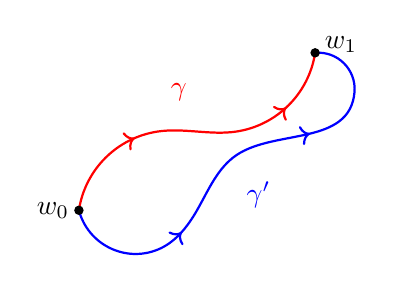
\begin{tikzpicture}
  % 曲線上に矢印を追加 (赤の曲線)
  \draw[red, 
        thick, 
        postaction={decorate}, 
        decoration={markings, 
                    mark=at position 0.3 with {\arrow{>}},
                    mark=at position 0.8 with {\arrow{>}}
                    }
        ]
    (0,0) to[out=80, in=130, curve through={(1,1) (2,1)}] (3,2) node[left] at (1.5,1.5) {$\gamma$};
  
  % 曲線上に矢印を追加 (青の曲線)
  \draw[blue,
        thick,
        postaction={decorate},
        decoration={markings,
                    mark=at position 0.3 with {\arrow{>}},
                    mark=at position 0.7 with {\arrow{>}}
                    }
        ]
    (0,0) to[out=-10, in=-30, curve through={(1,-0.5) (1.5,0) (2,0.7) (3.5,1.5)}] (3,2) node[right] at (2,0.2) {$\gamma'$};
  
  % 点の描画
  \fill (0,0) circle (0.6mm) node[left] {$w_{0}$};
  \fill (3,2) circle (0.6mm) node[right] at (3,2.1) {$w_{1}$};
\end{tikzpicture}
\end{center}


\Section{Cauchy's Integral Formula}
\Theorem{(Cauchy's Integral Formula1)\\
  $f$を閉円板$\overline{D(a;r)}$の近傍上の正則関数とし,円$C(a;r)$に
  反時計回りの向き(正の向き)を与える.このとき,次の等式が成り立つ.
  \begin{equation}
    f(z) = \frac{1}{2\pi i}\int_{C(a;r)}\frac{f(\zeta)}{\zeta - z}d\zeta\qquad (z\in D(a;r))
  \end{equation}
}{
  平行移動で$a = 0$とする.ある開円板$D(r')\ (r' > r)$上で
  $f$は正則である.$z\in D(r)$に対し$\varepsilon > 0$を$\overline{D(z;\varepsilon)}\subset D(r)$となるようにとる.
  今ここで,$C(r) = \partial D(r)$,$C(z;\varepsilon) = \partial D(z;\varepsilon)$
  は反時計回りの向き(正の向き)をもつ円とする.
  \begin{wrapfigure}{r}{0pt}
    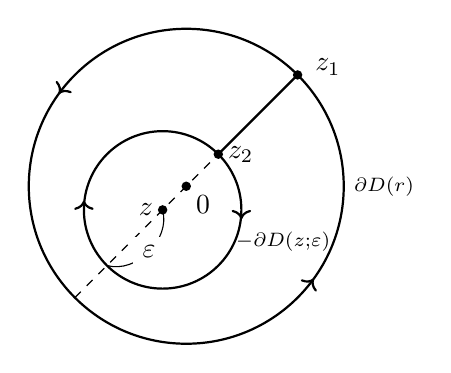
\begin{tikzpicture}
      \draw[dashed] (-1.414,-1.414) -- (1.414,1.414);
      \coordinate (z1) at (1.414,1.414);
      \coordinate (z2) at (0.407,0.407);
      \coordinate (center1) at (0,0);
      \coordinate (center2) at (-0.3,-0.3);
    
      \fill (z1) circle (0.6mm) node[right] at (1.514,1.514) {$z_{1}$};
      \fill (z2) circle (0.6mm) node[right] {$z_{2}$};
      \draw[thick,
            postaction={decorate},
            decoration={markings,
                        mark=at position 0.4 with {\arrow{>}},
                        mark=at position 0.9 with {\arrow{>}}
                        }
            ](center1) circle[radius = 2] node[right] at (2,0) {$\scriptstyle \partial D(r)$};
      \draw[thick,
            postaction={decorate},
            decoration={markings,
                        mark=at position 0.5 with {\arrow{<}},
                        mark=at position 1 with {\arrow{<}}
                        }
            ](center2) circle[radius = 1] node[right] at (0.5,-0.7) { $\scriptstyle -\partial D(z;\varepsilon)$};
      \fill (center1) circle (0.6mm) node[below right] {$0$};
      \fill (center2) circle (0.6mm) node[left] {$z$};
      \draw (-1.007,-1.007) to [bend right = 60] node [fill = white, midway] {$\varepsilon$} (center2);
      \draw[thick] (z1) to (z2);
    \end{tikzpicture}
    \caption{$\gamma$の図}
  \end{wrapfigure}
  ここで,右図(図B.1)のように曲線$\gamma$を定義する.\\
  具体的には次のように定義する.$z_{1}\in \partial D(r)$と
  $z_{2}\in \partial D(z;\varepsilon)$を最も遠くなるように取る.
  そして,$z_{1}$を始点として$z_{2}$へ動いて$\partial D(z;\varepsilon)$
  を時計回りに一周して($-\partial D(z;\varepsilon)$),次に$z_{2}$から$z_{1}$へ動いて,
  $\partial D(r)$を反時計回りに一周する曲線を$\gamma$とする.\\
  
}



\Section{Residue Theorem}

\Definition{
  領域$D$で正則な関数$f$が点$c\in D$で$f(c) = 0$ならば,$c$を$f$の\textbf{零点(zoro of $f$)}
  という.一致の定理によれば,$f$が恒等的に$0$でなければ,$f$の零点集合は内点を
  持たない.$c$を$f$の零点として$z = c$における$f$の冪級数展開を
  \begin{equation}
    f(z) = \sum_{n = 0}^{\infty}a_{n}(z - c)^{n}
  \end{equation}
  とする.$f(c) = 0$だから$a_{0} = 0$である.$f$は恒等的に$0$でないとするならば,
  $a_{n}$の中に$0$でないものがあるからそのような$a_{n}$の中で$n$が最小のものを
  $a_{k}$とする.このとき$f$は$c$において$k$位の零(zero of order $k$)を
  持つという.$k$を零点$c$の位数(order)または重複度(multiplicity)ということもある.
  定理〇〇によって,これは
  \begin{equation}
    f(c) = f'(c) = \dots = f^{(k-1)}(c) = 0\qquad (f^{(k)}(c)\neq 0)
  \end{equation}
  ということと同値である.
}

\Theorem{
  $f$は$D$上正則な関数で$z = c$において$k$位の零を持つとする.
  このとき$f(z) = (z - c)^{k}g(z),\ g(c) \neq 0$である$D$上の正則な関数$g$が存在する.
}{
  \begin{equation}
    g(z) = \frac{f(z)}{(z - c)^{k}}
  \end{equation}
  と定義すれば,$g$は$D\mysetminus \{c\}$で正則である.$f$の冪級数展開(B.39)を用いると,
  \begin{equation}
    \phi(z) := \frac{f(z)}{(z - c)^{k}} = \sum_{n = k}^{\infty}a_{n}(z - c)^{n - k}
  \end{equation}
  $\phi$はもとの冪級数と同じ収束半径を持つ.$\phi$の作り方から$\phi$は収束する領域内で
  $z \neq c$なる$z$に対して$g(z) = \phi(z)$が成立する.
  したがって,$g(c) = \phi(c)(=a_{k})$と定義すれば,$g$は$D$全体で正則で
  $f(z) = (z - c)^{k}g(z)$かつ$g(c)\neq 0$を満たす.
}

\Corollary{
  $f$が恒等的に$0$でないならば$f$の零点集合は離散的である.
}{
  $c$を$f$の零点とすれば,$f(z) = (z - c)^{k}g(z),\ g(c) \neq 0$なる$g$がある.
  $g(c) \neq 0$だから$c$の十分小さい近傍$U(c)$をとれば,$U(c)$の任意の点$z$に対して
  $g(z) \neq 0$である.したがって,$f$は$U(c)$内に$c$以外の零点を持たない.
  % 一致の定理から言える.
}

\Definition{
  領域$D$と$D$のりさん部分集合$\{c_{\alpha}\}_{\alpha\in A}$を考える.
  $f$は$D\mysetminus \{c_{\alpha}\}_{\alpha\in A}$で正則な関数とする.
  このとき$f$が$D$上の\textbf{有理型関数(meromorphic function)}であるとは,
  各$\alpha$に対して$c_{\alpha}$の近傍$U_{\alpha}$と$U_{\alpha}$で定義された
  正則関数$g_{\alpha},h_{\alpha}$が存在して,$U_{\alpha}\mysetminus c_{\alpha}$
  上で,
  \begin{equation}
    f(z) = \frac{g_{\alpha}(z)}{h_{\alpha}(z)}
  \end{equation}
  が成り立つことである.$z = c_{\alpha}$における$g_{\alpha},h_{\alpha}$の零点の位数を
  $k,l$とする.すると定理〇〇より
  \begin{equation}
    f(z) = \frac{g_{\alpha}(z)}{h_{\alpha}(z)} = \frac{(z - c_{\alpha})^{k}g'_{\alpha}(z)}{(z - c_{\alpha})^{l}h'_{\alpha}(z)}
  \end{equation}
  で$g'_{\alpha},h'_{\alpha}$は$z = c_{\alpha}$で$0$ではないようにとれる.
  よって,$k\geq l$ならば$f$は$z = c_{\alpha}$で正則になるように拡張できる.
  逆に$k < l$ならば$f$を$z = c_{\alpha}$まで正則にはできない.この場合$f$は
  $z = c_{\alpha}$で\textbf{極(pole)}を持つといって,$l - k$を極の位数(order)という.
}
$f$は$D$上の有理型関数で$z = c$で極を持つとする.$c$を中心とした十分小さい円周$C(c;\varepsilon)$をとって,積分
\begin{equation}
  \frac{1}{2\pi i}\int_{C(c;\varepsilon)}f(z)dz
\end{equation}
ただし,円周は正の向きに向き付けられているとする.Cauchyの積分定理によって,
正数$\varepsilon$が十分小さい時積分の値は$\varepsilon$のとり方によらない.
積分の値を$f$の$z = c$における\textbf{留数(residue)}といって,$\text{Res}(f,c)$とかく.\\
極の位数を$l$とすれば,$(z - c)^{l}f(z)$は点$c$まで正則に拡張できる.したがって,$f$は原点周りで,
\begin{equation}
  f(z) = \frac{a_{-l}}{(z - c)^{l}} + \frac{a_{-(l - 1)}}{(z - c)^{l - 1}} + \dots + \frac{a_{-1}}{z - c} + a_{0} + a_{1}z + a_{2}z^{2} + \dots
\end{equation}
と展開される.$0$次以上を$\varphi(z)$とおけば,
\begin{equation}
  f(z) = \sum_{n = 1}^{l}\frac{a_{-n}}{(z - c)^{n}} + \varphi(z)
\end{equation}
よって,両辺積分すれば,
\begin{equation}
  \int_{C(c;\varepsilon)}f(z)dz = \sum_{n = 1}^{l}a_{-n}\int_{C(c;\varepsilon)}\frac{1}{(z - c)^{n}}dz + \int_{C(c;\varepsilon)}\varphi(z)dz
\end{equation}
しかし$\varphi$は正則なので右辺の第二項は$0$で
\begin{equation}
  \int_{C(c;\varepsilon)}f(z)dz = \sum_{n = 1}^{l}a_{-n}\int_{C(c;\varepsilon)}\frac{1}{(z - c)^{n}}dz
\end{equation}
を得る.$z-c = \varepsilon e^{i\theta},\ (0\leq \theta \leq 2\pi)$とすれば,
\begin{align}
  \int_{C(c;\varepsilon)}\frac{1}{(z - c)^{n}}dz 
  &= \varepsilon^{1-n}i\int_{0}^{2\pi}e^{(1 - n)i\theta}d\theta\\
  &= \left\{
  \begin{alignedat}{2}
    &2\pi i \qquad &(n = 1)\\
    &0\qquad &(n \neq 1)
  \end{alignedat}
  \right.
\end{align}
である.ゆえに(B.49)の右辺で,$n = 1$の項のみが残り,
\begin{equation}
  \text{Res}(f,z) = a_{-1}
\end{equation}
となる.
\Theorem{(Residue Theorem)\\
  $D$を有界領域で$\partial D$が区分的に滑らかな単純閉曲線だとする.また$f$は$\overline{D}$
  を含む領域で定義された有利型関数で,境界$\partial D$上には極を持たないとする.
  このとき,
  \begin{equation}
    \frac{1}{2\pi i}\int_{\partial D}f(z)dz = \sum_{c}\mathrm{Res}(f,c)
  \end{equation}
  が成り立つ.ただし右辺の和は$D$内の$f$の極をすべて動く.
}{
  $\overline{D}$はコンパクトなので,$D$内の極は有限個しかない.極$c$の
  まわりに十分小さい円周を考えてCauchyの積分定理を適用すれば求める等式を得る.
}




\Section{Several Variables}
$\mathbf{C}^{n}$の領域$D$上で定義された関数$f$を考える.$z = (z_{1},\dots,z_{n}) \in \mathbf{C}^{n}$をとる.\\
$x_{j} = \Re z_{j},\ y_{j} = \Im z_{j}\ (j = 1,\dots ,n)$として,
一変数の場合と同様に,
\begin{align}
  \frac{\partial}{\partial z_{j}} =\frac{1}{2}\left( \frac{\partial}{\partial x_{j}} + \frac{1}{i}\frac{\partial}{\partial y_{j}} \right)\\
  \frac{\partial}{\partial \overline{z_{j}}} =\frac{1}{2}\left( \frac{\partial}{\partial x_{j}} - \frac{1}{i}\frac{\partial}{\partial y_{j}}\right)
\end{align}
と定義する.$f$が$(x_{1},y_{1},x_{2},y_{2},\dots,x_{n},y_{n})$について$C^{1}$級で
$D$上で
\begin{equation}
  \frac{\partial f}{\partial \overline{z_{j}}} = 0 \qquad (j = 1,\dots,n)
\end{equation}
を満たすとき$f$は$D$で\textbf{正則(holomorphic)}という.あるいは$f$は$D$上の
\textbf{正則関数(holomorphic function)}と呼ばれる.\\
次に一次元の円板$D\subset \mathbf{C}$に相当する多重円板を定義する.\\
$c = (c_{1},\dots,c_{n}) \in \mathbf{C}^{n}$,$r= (r_{1},\dots,r_{n}) \in (\mathbf{R}_{>0})^{n}$に対して,
\begin{equation}
  \Delta(c;r) = \{z = (z_{1},\dots,z_{n}) \in \mathbf{C}^{n} \mid |z_{j} - c_{j}| < r_{j},\ j = 1,\dots ,n\} = D(c_{1};r_{1})\times \dots \times D(c_{n};r_{n})
\end{equation}
の形の領域を$c$を中心とする\textbf{多重円板(polydisc/polydisk)}という.\\
$f(z) = f(z_{1},\dots ,z_{n})$は多重円板$\Delta(c;r)$の閉包$\overline{\Delta(c;r)}$を
含む領域で正則な関数とする.$(z_{2},\dots,z_{n})$を固定して$z_{1}$に関して
一変数のCauchyの積分公式を用いれば,$(z_{1},\dots,z_{n}) \in \Delta$に対して
\begin{equation}
  f(z_{1},\dots,z_{n}) = \frac{1}{2\pi i}\int_{D(c_{1};r_{1})}\frac{f(\zeta_{1},z_{2},\dots,z_{n})}{\zeta_{1} - z_{1}}d\zeta_{1}
\end{equation}
である.ただし円板$D(c_{1};r_{1})$は正の向きに向き付けられているとする.
これを$z_{2},\dots,z_{n}$に繰り返し適用すれば,
\begin{align*}
  f(z_{1},\dots,z_{n}) 
  &= \frac{1}{2\pi i}\int_{D(c_{1};r_{1})}\frac{f(\zeta_{1},z_{2},\dots,z_{n})}{\zeta_{1} - z_{1}}d\zeta_{1}\\
  &= \left(\frac{1}{2\pi i}\right)^{2}\int_{D(c_{1};r_{1})}\int_{D(c_{2};r_{2})}\frac{f(\zeta_{1},\zeta_{2},z_{3},\dots,z_{n})}{(\zeta_{2} - z_{2})(\zeta_{1} - z_{1})}d\zeta_{2}d\zeta_{1}\\
  &= \left(\frac{1}{2\pi i}\right)^{n}\int_{D(c_{1};r_{1})}\dots \int_{D(c_{n};r_{n})}\frac{f(\zeta_{1},\dots,\zeta_{n})}{(\zeta_{n} - z_{n})\dots (\zeta_{1} - z_{1})}d\zeta_{n} \dots d\zeta_{1}\\
\end{align*}
と書くことが出来る.\\
$n$変数の場合,$c = (c_{1},\dots,c_{n}) \in \mathbf{C}^{n}$における冪級数は
\begin{equation}
  \sum_{m_{1} = 0}^{\infty}\dots \sum_{m_{n} = 0}^{\infty}a_{m_{1},\dots,m_{n}}(z_{1} - c_{1})^{m_{1}}\dots (z_{n} - c_{n})^{m_{n}}
\end{equation}
である.一変数の場合と同様にして,$\mathbf{C}^{n}$の領域$D$で正則な関数$f$は
$D$の各点$c$の近傍で絶対収束する冪級数に展開される.このとき展開の係数は
\begin{align}
  a_{m_{1},\dots,m_{n}} 
  &= \frac{1}{m_{1}!\dots m_{n}!}\frac{\partial^{m_{1} + \dots + m_{n}}f}{\partial z_{1}^{m_{1}}\dots \partial z_{n}^{m_{n}}}(c)\\
  &= \left(\frac{1}{2\pi i}\right)^{n}\int_{D(c_{1};r_{1})}\dots \int_{D(c_{n};r_{n})}\frac{f(\zeta_{1},\dots,\zeta_{n})}{(\zeta_{n} - c_{n})^{m_{n} + 1}\dots (\zeta_{1} - c_{1})^{m_{1} + 1}}d\zeta_{n}\dots d\zeta_{1}
\end{align}
で与えられる.したがって$D(c_{1};r_{1})\times \dots \times D(c_{n};r_{n})$における
$|f(z_{1},\dots,z_{n})|$の最大値を$M$とすれば,
\begin{equation}
  |a_{m_{1},\dots,m_{n}}|\leq \frac{M}{r_{1}^{m_{1}}\dots r_{n}^{m_{n}}}
\end{equation}
が成り立つ.特に$r_{1},\dots,r_{n}$の最小値を$r$とすれば,
\begin{equation}
  |a_{m_{1},\dots,m_{n}}|\leq \frac{M}{r^{m_{1}+\dots + m_{n}}}
\end{equation}
が成り立つ.
一変数の場合と同様に,これらの結果を用いて一致の定理と最大値の原理が証明される.
\Theorem{(Hartogs' Theorem)
  $D$を$\mathbf{C}^{n}$の原点$0$を含む領域で$n\geq 2$とする.$f$が$D\mysetminus \{0\}$
  で定義された正則関数ならば$f$は$D$上の正則関数に拡張される.
}{
  $D$は多重円板$\{z \in \mathbf{C}^{n}\mid |z_{j}| < r_{j},\ j = 1,\dots,n\}$
  としてよい.正数$s$を$0 < s < r_{1}$となるように選び
  \begin{equation}
    g(z_{1},\dots,z_{n}) = \frac{1}{2\pi i}\int_{D(0;s)}\frac{f(\zeta_{1},z_{2},\dots,z_{n})}{\zeta_{1} - z_{1}}d\zeta_{1}
  \end{equation}
  と定義する.ここで$D(0;s)$は正の向きに向き付けられているとする.このとき
  $g$は$D' = \{z \in \mathbf{C}^{n} \mid |z_{1}| < s,\ |z_{j}| < r_{j},\ j = 2,\dots,n\}$
  で正則な関数を定める.
}

\printindex
\end{document}